\documentclass[12pt, a4paper]{article}

% --- Pakiety ---
\usepackage[utf8]{inputenc}
\usepackage[T1]{fontenc}
\usepackage[polish]{babel}
\usepackage{geometry}
\usepackage{amsmath}
\usepackage{amssymb}
\usepackage{graphicx}
\usepackage{booktabs}
\usepackage{siunitx}
\usepackage{caption}
\usepackage{subcaption}
\usepackage{float}
\usepackage{hyperref}
\hypersetup{hidelinks}
\usepackage{xcolor}
\usepackage{array}
\usepackage{multirow}
\usepackage{fancyhdr}

% --- Marginesy ---
\geometry{
    top=2.5cm,
    bottom=2.5cm,
    left=2.5cm,
    right=2.5cm,
    footskip=2cm
}

% --- Stopka ---
\pagestyle{fancy}
\fancyhf{}
\renewcommand{\headrulewidth}{0pt}
\renewcommand{\footrulewidth}{0.4pt}
\fancyfoot[R]{
\includegraphics[height=0.8cm]{lumon.pdf}}

% --- Konfiguracja siunitx ---
\sisetup{
    output-decimal-marker = {,},
    separate-uncertainty = true
}

% --- Dane raportu ---
\newcommand{\tytul}{Badanie zjawiska dyfrakcji i interferencji światła laserowego}
\newcommand{\codeword}{Bodo}
\newcommand{\nrCwiczenia}{O18}
\newcommand{\autor}{Karol Peszek}
\newcommand{\nrGrupy}{A}
\newcommand{\dataWykonania}{27 października i 3 listopada 2026}

% --- Tytuł dokumentu ---
\title{
    \large I Pracownia Fizyczna \\[0.5em]
    \textbf{Ćwiczenie \nrCwiczenia} \\[0.3em]
    \LARGE \tytul\space,,\codeword''
}
\author{
    \autor\\
     Grupa \nrGrupy}
\date{
    Data wykonania pomiarów: \dataWykonania\\
}

% =============================================
\begin{document}
% =============================================

\maketitle
\thispagestyle{empty}
\newpage

% -------------------------------------------
\section{Cel ćwiczenia}
% -------------------------------------------

W niniejszej pracy zbadano rozkład natężenia światła w obrazach dyfrakcyjnych pojedynczej
szczeliny, dwóch szczelin oraz układów $N = 2$--$5$ szczelin, oświetlonych światłem
lasera czerwonego i zielonego. Rozkłady zarejestrowano skanerem przesuwanym w poprzek
obrazu. Na ich podstawie wyznaczono szerokości szczelin $a$ i odległości między szczelinami
$d$ dwiema metodami: dopasowania krzywej natężenia oraz regresji liniowej położeń minimów
i maksimów w funkcji ich rzędu. Dodatkowo zbadano, jak obraz zmienia się z odległością
szczelina--detektor i z szerokością apertury czujnika, oraz porównano obrazy tych samych
szczelin dla obu laserów. Wykazano, że przelicznik położenia skanera użyty przez program
akwizycji zaniża przesunięcia, i skalibrowano go na podstawie zakresu przesuwu skanera.

% -------------------------------------------
\section{Wstęp teoretyczny}
% -------------------------------------------

\subsection{Interferencja światła na dwóch szczelinach}

Interferencja polega na nakładaniu się fal, które prowadzi do stałego w czasie
przestrzennego rozkładu natężenia fali wypadkowej: jasnych prążków (interferencja
konstruktywna) i ciemnych (destruktywna). Stały obraz powstaje dla fal spójnych, czyli
o stałej w czasie różnicy faz. Gdy światło jest dodatkowo monochromatyczne, jak światło
lasera, prążki wszystkich rzędów leżą w tych samych miejscach i są wyraźne daleko od środka
obrazu~\cite{skrypt}.

W doświadczeniu Younga (Rysunek~\ref{fig:young}) światło z dwóch wąskich szczelin
$S_1$, $S_2$ odległych o $d$ dociera do punktu $P$ ekranu odległego o $D$. Różnica dróg
optycznych wynosi $r_2 - r_1 = d\sin\theta$, a maksimum natężenia powstaje, gdy jest ona
całkowitą wielokrotnością długości fali~\cite{skrypt}:
\begin{equation}
    d\sin\theta = m\lambda, \qquad m = 0, \pm1, \pm2, \dots
    \label{eq:young_max}
\end{equation}
gdzie $m$ --- rząd maksimum. Dla $D \gg d$ można przyjąć $\sin\theta \approx \operatorname{tg}\theta
= y/D$, gdzie $y$ --- odległość od środka obrazu, skąd położenie maksimum $m$-tego rzędu
\begin{equation}
    y_m = \frac{\lambda D}{d}\,m.
    \label{eq:young_y}
\end{equation}

\begin{figure}[H]
    \centering
    \begin{subfigure}{0.48\textwidth}
        \centering
        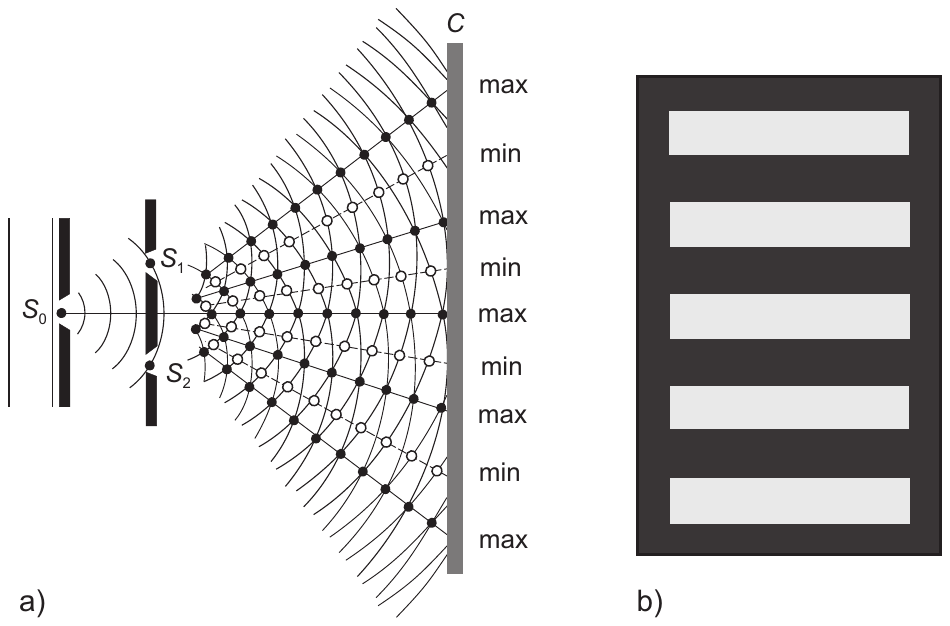
\includegraphics[width=\textwidth]{young_experiment.png}
        \caption{}
    \end{subfigure}
    \hfill
    \begin{subfigure}{0.48\textwidth}
        \centering
        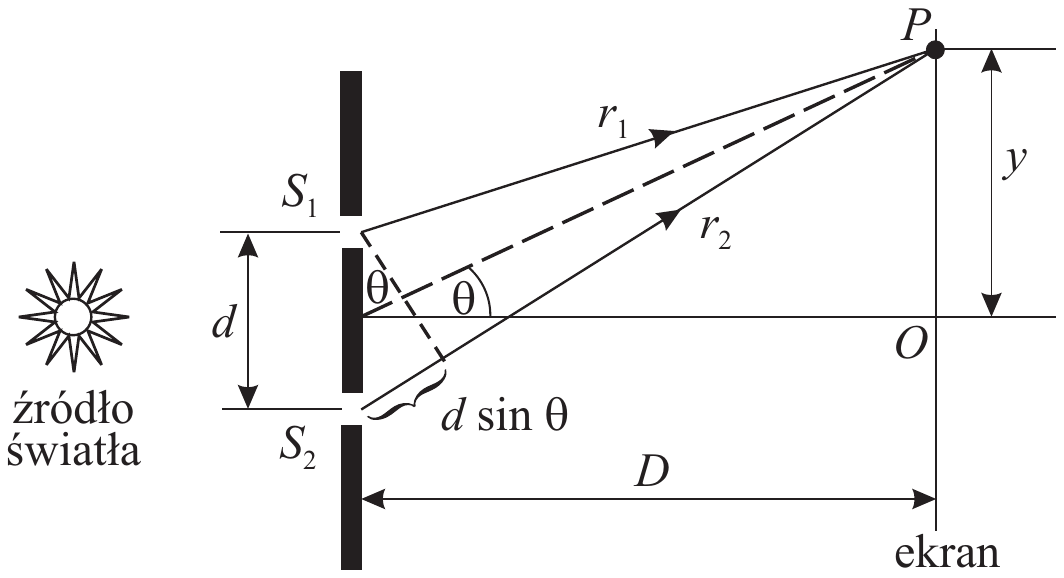
\includegraphics[width=\textwidth]{young_geometry.png}
        \caption{}
    \end{subfigure}
    \caption{Doświadczenie Younga: (a) schemat i obraz prążków interferencyjnych,
             (b) konstrukcja geometryczna --- różnica dróg optycznych $d\sin\theta$
             fal z szczelin $S_1$ i $S_2$ w punkcie $P$ ekranu. Źródło:~\cite{skrypt}.}
    \label{fig:young}
\end{figure}

Natężenie światła jest proporcjonalne do kwadratu amplitudy pola elektrycznego.
Pole każdej z fal można przedstawić jako wektor o długości $E_0$ obracający się
z częstością $\omega$, a pole wypadkowe --- jako sumę takich wektorów przesuniętych
o różnicę faz $\Phi = \frac{2\pi}{\lambda} d\sin\theta$ (Rysunek~\ref{fig:phasors}a).
Dla dwóch szczelin amplituda wypadkowa wynosi $E_w = 2E_0\cos(\Phi/2)$, więc~\cite{skrypt}
\begin{equation}
    I_\theta = I_\text{max}\cos^2\!\left(\frac{\pi d}{\lambda}\sin\theta\right),
    \label{eq:two_slits}
\end{equation}
gdzie $I_\text{max} = 4I_0$ --- natężenie maksimum zerowego rzędu, $I_0$ --- natężenie fali
z jednej szczeliny (Rysunek~\ref{fig:phasors}b). Sumowanie $N$ wektorów o stałej różnicy faz
daje rozkład dla $N$ wąskich szczelin~\cite{skrypt}:
\begin{equation}
    I_\theta = I_0\left[\frac{\sin\!\left(N\frac{\pi d}{\lambda}\sin\theta\right)}
                             {\sin\!\left(\frac{\pi d}{\lambda}\sin\theta\right)}\right]^2.
    \label{eq:n_slits}
\end{equation}
Położenia maksimów głównych nie zależą od $N$ i są dane wzorem~\eqref{eq:young_max}.
Ze wzrostem $N$ maksima główne stają się węższe, a między każdymi dwoma sąsiednimi
pojawia się $N - 2$ słabych maksimów pobocznych (Rysunek~\ref{fig:n_slits}).

\begin{figure}[H]
    \centering
    \begin{subfigure}{0.48\textwidth}
        \centering
        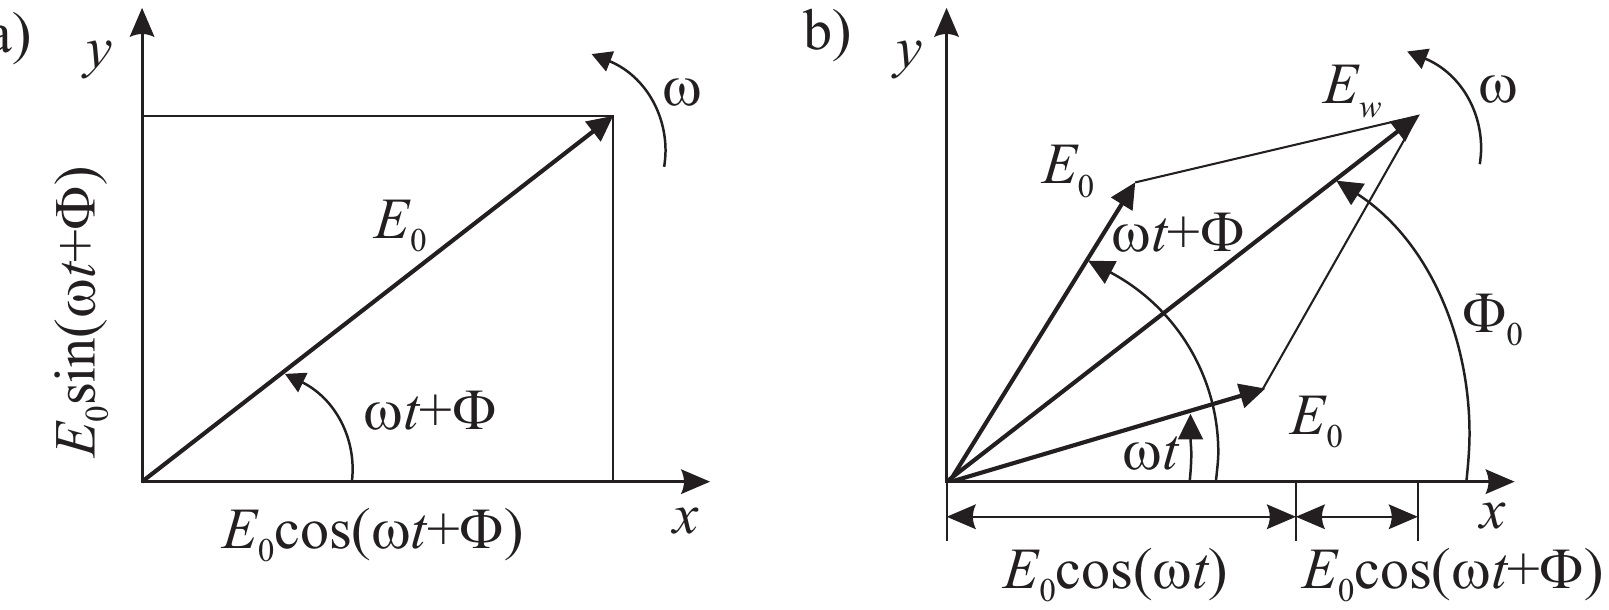
\includegraphics[width=\textwidth]{electric_field_vector.png}
        \caption{}
    \end{subfigure}
    \hfill
    \begin{subfigure}{0.48\textwidth}
        \centering
        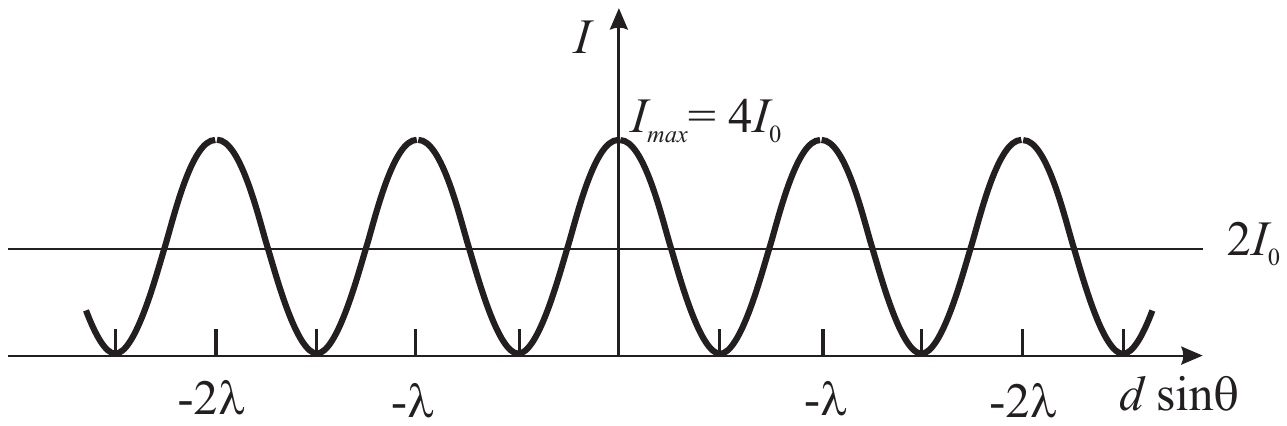
\includegraphics[width=\textwidth]{amplitudes.png}
        \caption{}
    \end{subfigure}
    \caption{(a) Wektor natężenia pola elektrycznego jako obracający się wektor i konstrukcja
             amplitudy wypadkowej dla dwóch fal o różnicy faz $\Phi$; (b) rozkład natężenia
             dla dwóch wąskich szczelin, wzór~\eqref{eq:two_slits}; $2I_0$ --- natężenie
             średnie. Źródło:~\cite{skrypt}; w oryginale na osi po prawej stronie błędnie
             $-\lambda$, $-2\lambda$ --- powinno być $\lambda$, $2\lambda$.}
    \label{fig:phasors}
\end{figure}

\begin{figure}[H]
    \centering
    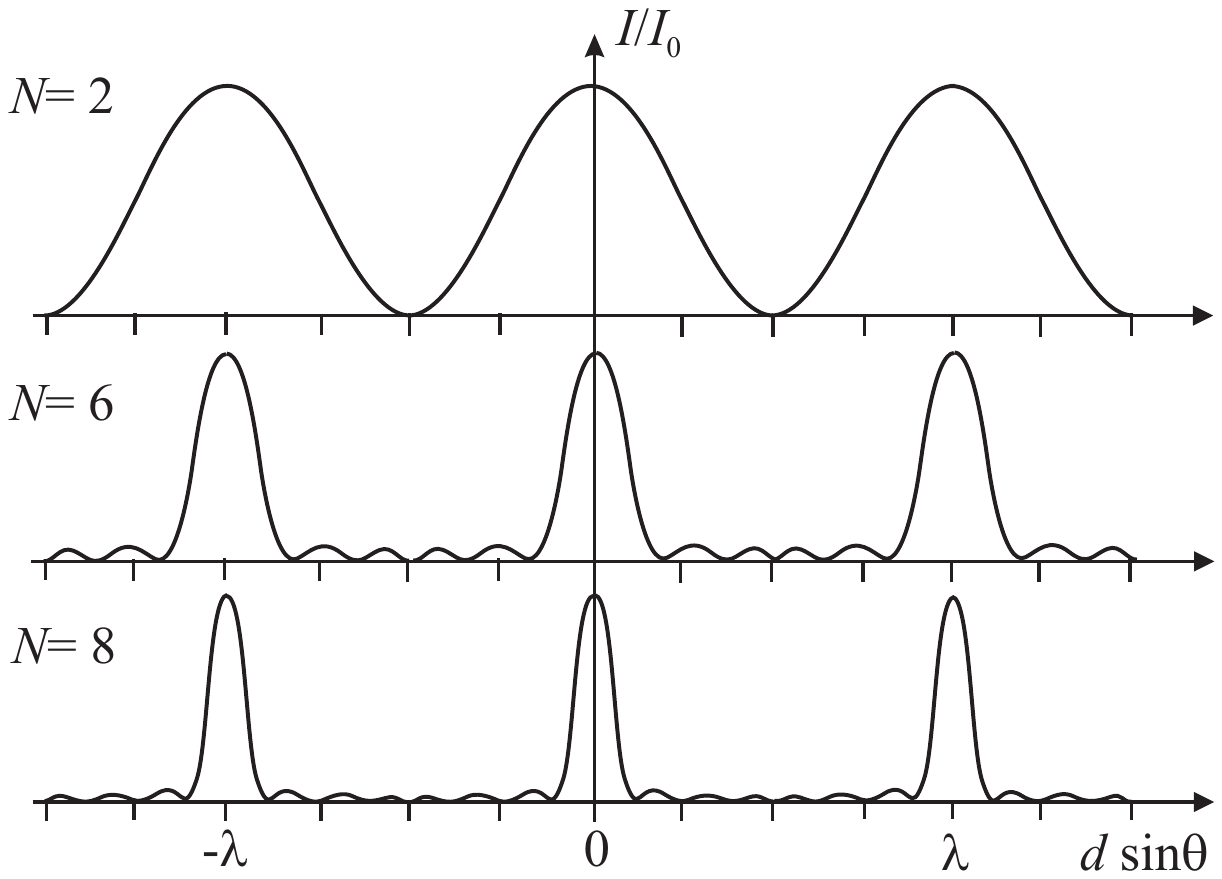
\includegraphics[width=0.6\textwidth]{multi_slit_amplitudes.png}
    \caption{Rozkład natężenia dla $N = 2$, $6$ i $8$ wąskich szczelin,
             wzór~\eqref{eq:n_slits} (bez czynnika dyfrakcyjnego). Źródło:~\cite{skrypt}.}
    \label{fig:n_slits}
\end{figure}

\subsection{Dyfrakcja na pojedynczej szczelinie}

Za szczeliną światło przechodzi także w obszar cienia geometrycznego --- zachodzi dyfrakcja
(Rysunek~\ref{fig:diffraction}a). Kąt ugięcia jest rzędu $\lambda/a$, więc efekt jest
wyraźny, gdy szerokość szczeliny nie jest dużo większa od długości fali (w ćwiczeniu
$a/\lambda \approx 30$--$250$, kąty ugięcia rzędu stopnia).
Zgodnie z zasadą Huygensa każdy punkt czoła fali w obrębie szczeliny jest źródłem fali
kulistej, a obraz dyfrakcyjny jest wynikiem interferencji tych fal. W ćwiczeniu zachodzi
dyfrakcja Fraunhofera: wiązka laserowa jest równoległa, a detektor znajduje się w polu
dalekim, $D \gg L^2/\lambda$, gdzie $L$ --- rozmiar całej struktury~\cite{skrypt}. Dla
najszerszej pojedynczej szczeliny ($L = a = 0{,}16$~mm) $L^2/\lambda \approx 39$~mm wobec
$D = 900$~mm. Dla par i układów $N$ szczelin warunek jest spełniony słabiej (omówienie
w Opracowaniu).

Po podzieleniu szczeliny na dwie połowy (Rysunek~\ref{fig:diffraction}b) fale z par punktów
odległych o $a/2$ wygaszają się, gdy różnica ich dróg wynosi $\lambda/2$. Prowadzi to
do warunku na minima natężenia~\cite{skrypt}:
\begin{equation}
    a\sin\theta = m\lambda, \qquad m = \pm1, \pm2, \dots
    \label{eq:single_min}
\end{equation}
Sumowanie wektorów pola od nieskończenie wielu pasków szczeliny
(Rysunek~\ref{fig:fraunhofer}a) daje rozkład natężenia~\cite{skrypt}
\begin{equation}
    I_\theta = I_0\left[\frac{\sin\!\left(\frac{\pi a}{\lambda}\sin\theta\right)}
                             {\frac{\pi a}{\lambda}\sin\theta}\right]^2,
    \label{eq:single_slit}
\end{equation}
gdzie $I_0$ --- natężenie maksimum centralnego ($\theta = 0$). Maksimum centralne jest
dwa razy szersze od pozostałych i znacznie od nich silniejsze
(Rysunek~\ref{fig:fraunhofer}b). Im węższa szczelina, tym szerszy obraz i rzadsze minima.

\begin{figure}[H]
    \centering
    \begin{subfigure}{0.48\textwidth}
        \centering
        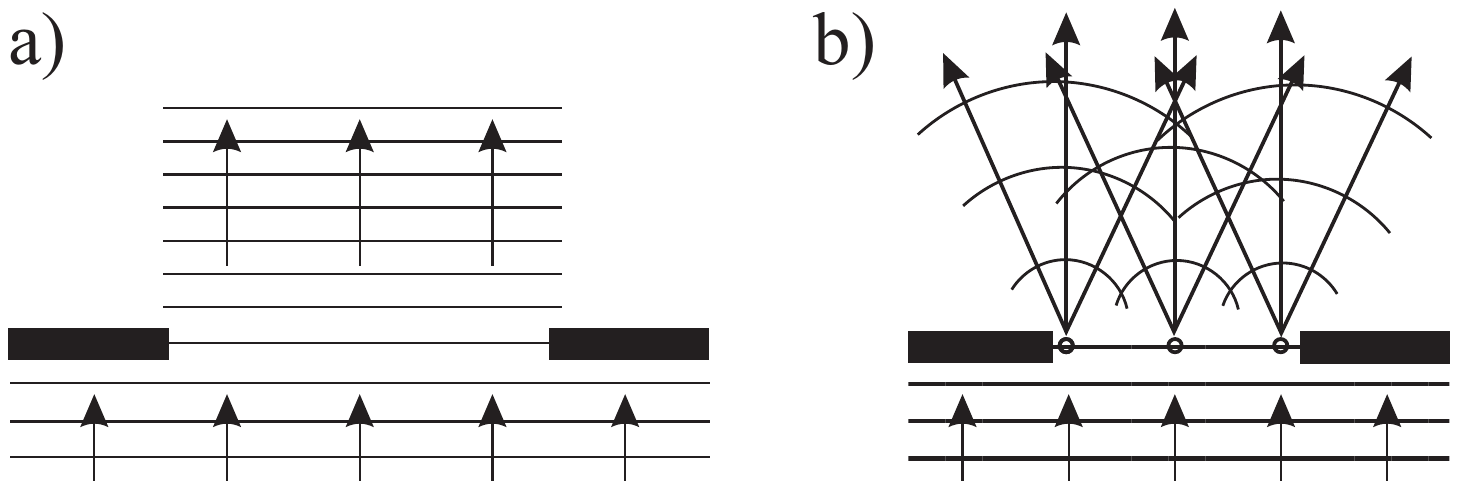
\includegraphics[width=\textwidth]{difraction.png}
        \caption{}
    \end{subfigure}
    \hfill
    \begin{subfigure}{0.48\textwidth}
        \centering
        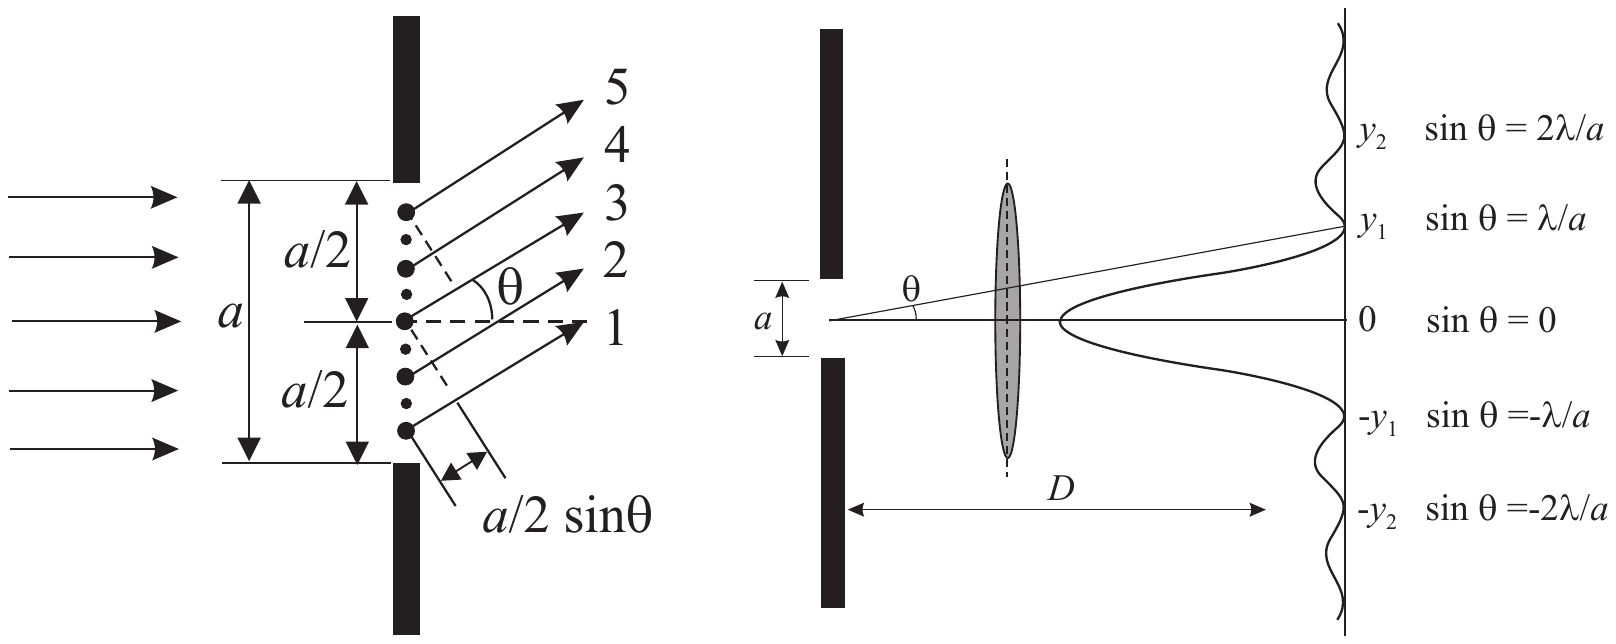
\includegraphics[width=\textwidth]{signle_slit_diffraction.png}
        \caption{}
    \end{subfigure}
    \caption{(a) Rozkład światła za szeroką szczeliną i za szczeliną o szerokości porównywalnej
             z długością fali; (b) podział szczeliny na połowy i obraz dyfrakcyjny
             pojedynczej szczeliny w odległości $D$. Źródło:~\cite{skrypt}.}
    \label{fig:diffraction}
\end{figure}

\begin{figure}[H]
    \centering
    \begin{subfigure}{0.55\textwidth}
        \centering
        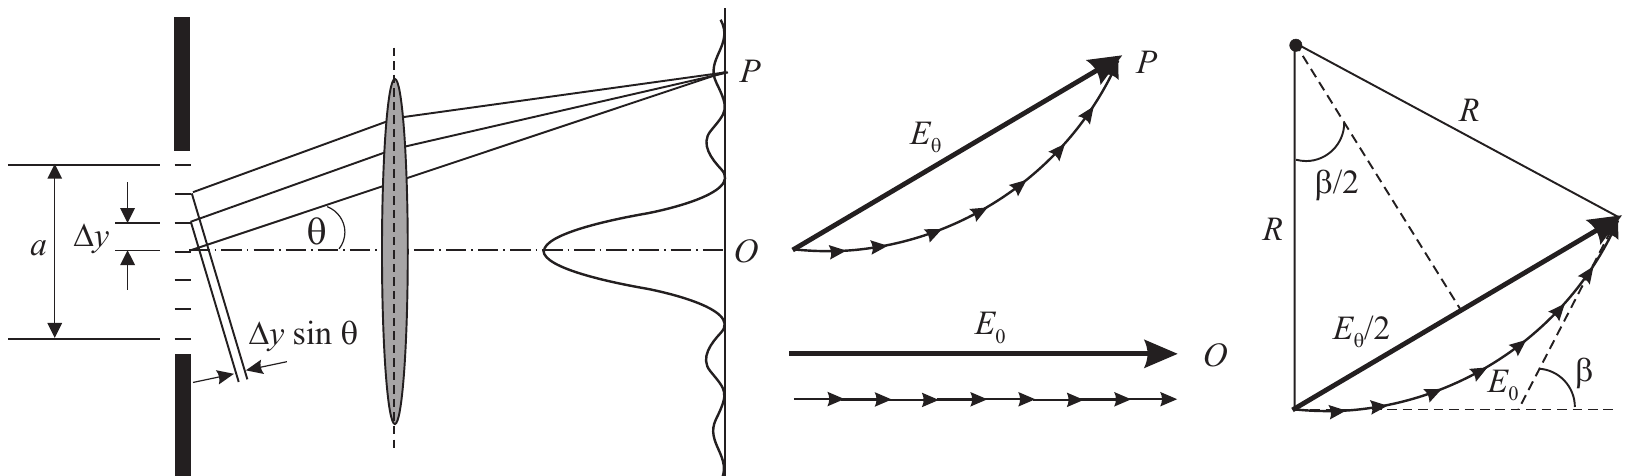
\includegraphics[width=\textwidth]{frauenhofer_difraction.png}
        \caption{}
    \end{subfigure}
    \hfill
    \begin{subfigure}{0.4\textwidth}
        \centering
        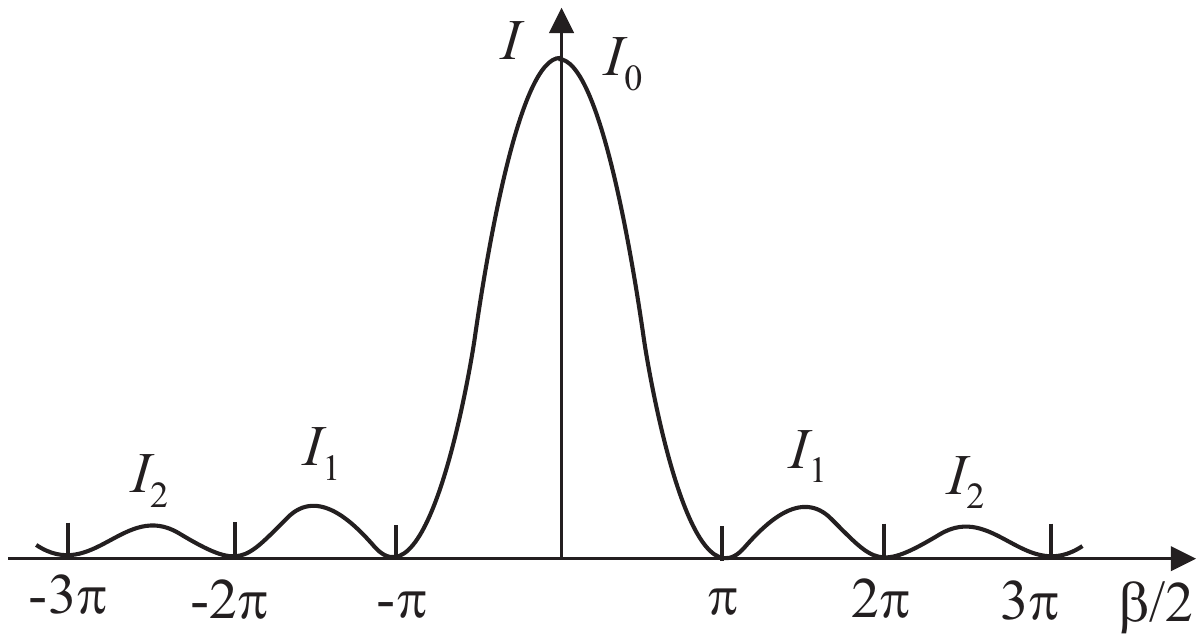
\includegraphics[width=\textwidth]{frauenhofer_difraction_amplitude.png}
        \caption{}
    \end{subfigure}
    \caption{Dyfrakcja Fraunhofera na pojedynczej szczelinie: (a) konstrukcja amplitudy
             wypadkowej $E_\theta$ z wektorów pola od kolejnych pasków szczeliny,
             (b) rozkład natężenia, wzór~\eqref{eq:single_slit}. Źródło:~\cite{skrypt}.}
    \label{fig:fraunhofer}
\end{figure}

\subsection{Dyfrakcja i interferencja na układzie $N$ szczelin}

Dla $N$ szczelin o skończonej szerokości $a$ obraz interferencyjny jest modulowany
obrazem dyfrakcyjnym pojedynczej szczeliny, a rozkład natężenia jest iloczynem
wzorów~\eqref{eq:n_slits} i~\eqref{eq:single_slit}~\cite{skrypt}:
\begin{equation}
    I_\theta = I_0\left[\frac{\sin\!\left(N\frac{\pi d}{\lambda}\sin\theta\right)}
                             {\sin\!\left(\frac{\pi d}{\lambda}\sin\theta\right)}\right]^2
               \left[\frac{\sin\!\left(\frac{\pi a}{\lambda}\sin\theta\right)}
                          {\frac{\pi a}{\lambda}\sin\theta}\right]^2.
    \label{eq:full}
\end{equation}
Położenia maksimów głównych~\eqref{eq:young_max} i minimów obwiedni
dyfrakcyjnej~\eqref{eq:single_min} nie zależą od $N$ (Rysunek~\ref{fig:full}). Dla
$N = 2$ pierwszy czynnik przechodzi w $4\cos^2\!\left(\frac{\pi d}{\lambda}\sin\theta\right)$,
a w maksimum centralnym obwiedni mieści się $2d/a - 1$ prążków (dla całkowitego $d/a$,
gdy prążki $m' = \pm d/a$ trafiają w zera obwiedni i znikają).

\begin{figure}[H]
    \centering
    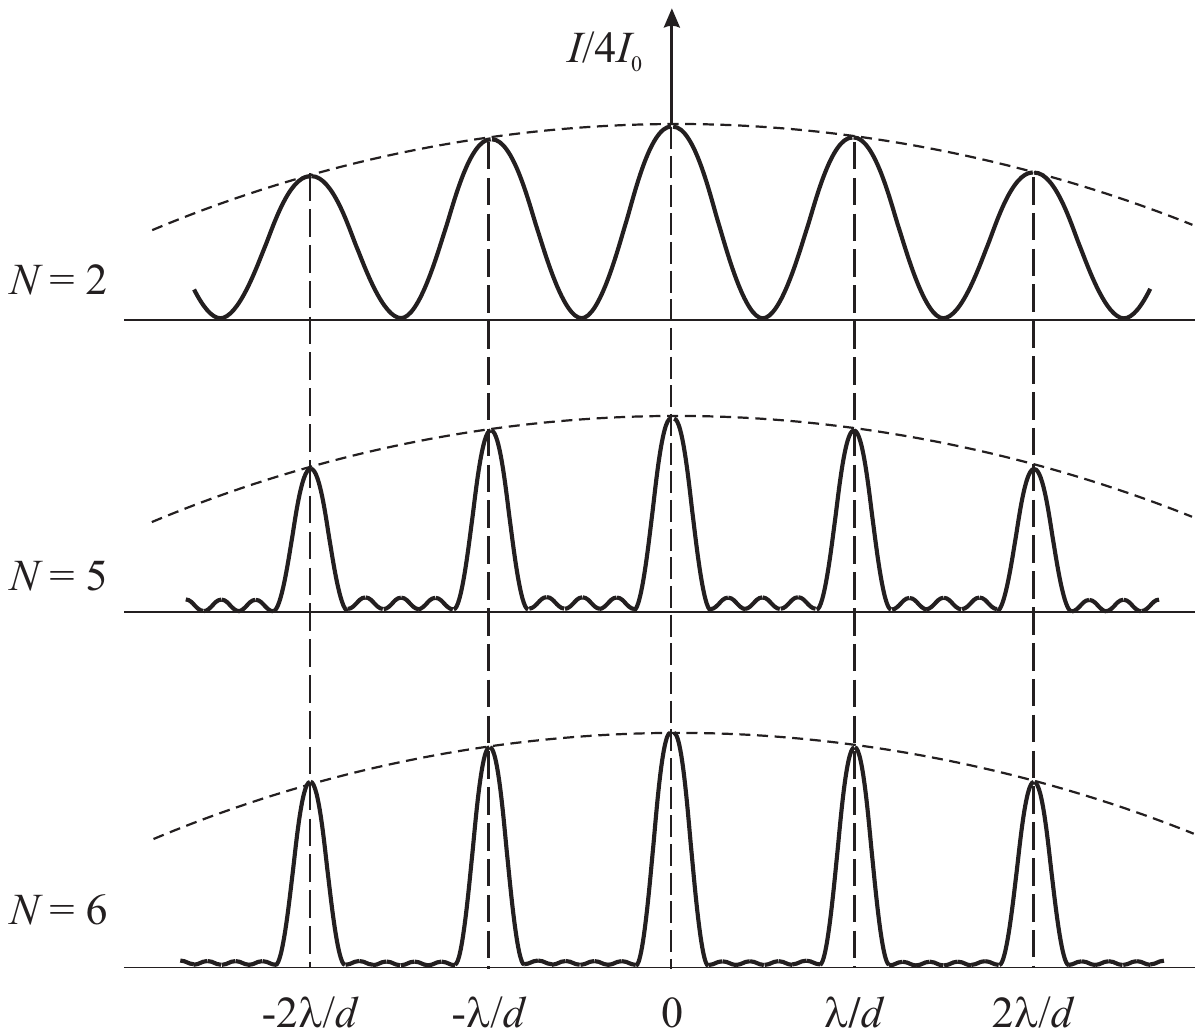
\includegraphics[width=0.6\textwidth]{multi_slit_intensity_distribution.png}
    \caption{Rozkład natężenia dla $N = 2$, $5$ i $6$ szczelin o tej samej szerokości $a$
             i odległości $d$; linia przerywana --- obwiednia dyfrakcyjna.
             Źródło:~\cite{skrypt}.}
    \label{fig:full}
\end{figure}

\subsection{Wyznaczanie szerokości i odległości szczelin}
\label{sec:method}

Z warunku~\eqref{eq:single_min} i przybliżenia $\sin\theta \approx \operatorname{tg}\theta
= x_m/D$ (Rysunek~\ref{fig:slit_width}) położenie $m$-tego minimum dyfrakcyjnego
względem środka obrazu wynosi~\cite{skrypt}
\begin{equation}
    x_m = \frac{\lambda D}{a}\,m,
    \label{eq:minima}
\end{equation}
a położenie maksimów interferencyjnych opisuje wzór~\eqref{eq:young_y} z $d$ w miejsce $a$.
Położenie środka obrazu $x_0$ na osi skanera jest nieznane.
Zależność $x_m = x_0 + (\lambda D/a)\,m$ jest liniowa w rzędzie $m$, a z jej nachylenia
$s = \lambda D/a$ wyznacza się $a = \lambda D/s$ (analogicznie $d$)~\cite{dodatek}.

Druga metoda to dopasowanie wzoru~\eqref{eq:full} do całego rozkładu $I(x)$. Z oznaczeniami
$y = x - C$ ($C$ --- środek obrazu na osi skanera) i
\begin{equation}
    B_a = \frac{\pi a}{\lambda D}, \qquad B_d = \frac{\pi d}{\lambda D}
    \label{eq:B}
\end{equation}
dla pojedynczej szczeliny model ma postać~\cite{dodatek}
\begin{equation}
    I(x) = A\left[\frac{\sin(B_a y)}{B_a y}\right]^2 + b,
    \label{eq:model_single}
\end{equation}
a dla $N$ szczelin
\begin{equation}
    I(x) = A\left[\frac{\sin(N B_d y)}{N\sin(B_d y)}\right]^2
             \left[\frac{\sin(B_a y)}{B_a y}\right]^2 + b,
    \label{eq:model_multi}
\end{equation}
gdzie $A$ --- natężenie maksimum centralnego, $b$ --- stałe tło. Z dopasowanych
$B_a$ i $B_d$ otrzymuje się $a = B_a\lambda D/\pi$ oraz $d = B_d\lambda D/\pi$.

\begin{figure}[H]
    \centering
    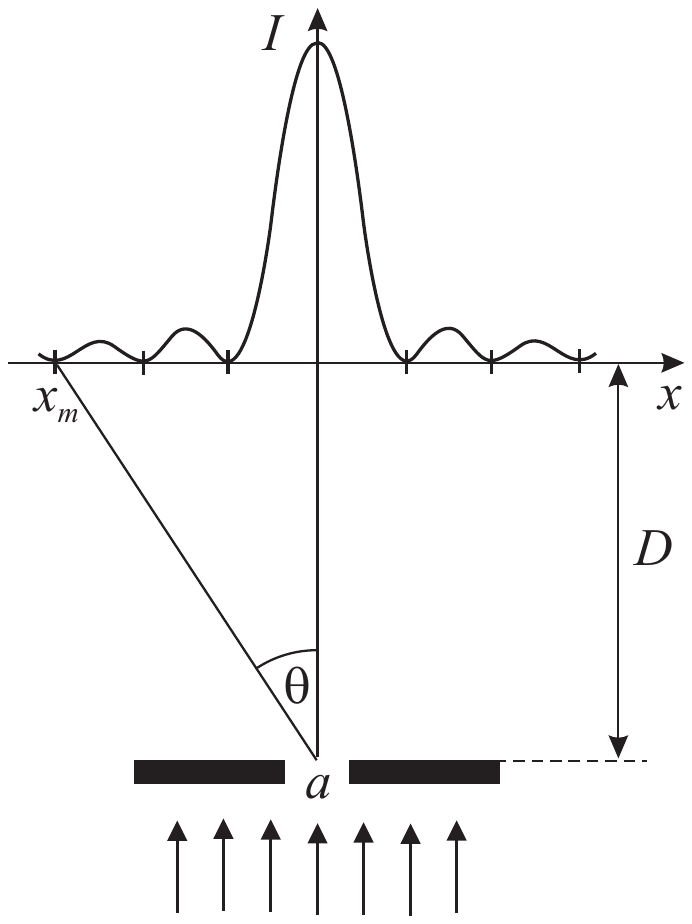
\includegraphics[width=0.35\textwidth]{slit_width.png}
    \caption{Wyznaczanie szerokości szczeliny: $x_m$ --- położenie minimum względem środka
             obrazu, $D$ --- odległość szczelina--detektor. Źródło:~\cite{skrypt}.}
    \label{fig:slit_width}
\end{figure}

\subsection{Przyjęte wartości}

Długości fal odczytano z tabliczek znamionowych laserów PASCO: $\lambda_\text{red} = 650$~nm
i $\lambda_\text{green} = 515$~nm (skrypt podaje dla lasera czerwonego 640~nm~\cite{skrypt}).
Tabliczki nie podają tolerancji, dlatego dla obu laserów przyjęto $u_\lambda = 5$~nm ---
typową tolerancję laserów diodowych (np.\ $650 \pm 5$~nm dla lasera 3B Scientific
U22000~\cite{laser3b}). Nominalne wymiary szczelin podano na tarczy producenta:
$a = 0{,}02;\ 0{,}04;\ 0{,}08;\ 0{,}16$~mm dla pojedynczych szczelin,
$a \in \{0{,}04;\ 0{,}08\}$~mm i $d \in \{0{,}25;\ 0{,}50\}$~mm dla par oraz $a = 0{,}04$~mm,
$d = 0{,}125$~mm dla układów $N$ szczelin~\cite{dodatek}.

% -------------------------------------------
\section{Opis układu pomiarowego}
% -------------------------------------------

Układ pomiarowy przedstawiono na Rysunku~\ref{fig:setup}. Na ławie optycznej ze skalą
ustawiono kolejno: laser (z lewej), uchwyt z tarczą szczelin i skaner dyfrakcyjny
(z prawej). Wiązka lasera pada prostopadle na wybrany układ szczelin, a obraz dyfrakcyjny
powstaje w płaszczyźnie szczeliny wejściowej czujnika skanera. Skaner przesuwa się ręcznie,
korbką, w poprzek obrazu. Enkoder obrotowy mierzy jego położenie $x$, a czujnik światła ---
natężenie $I$. Skaner łączył się przez Bluetooth z komputerem, na którym program w Pythonie
(biblioteka \texttt{pasco}) odczytywał na żądanie pary $(x, I)$ i zapisywał je do plików CSV.

\begin{figure}[H]
    \centering
    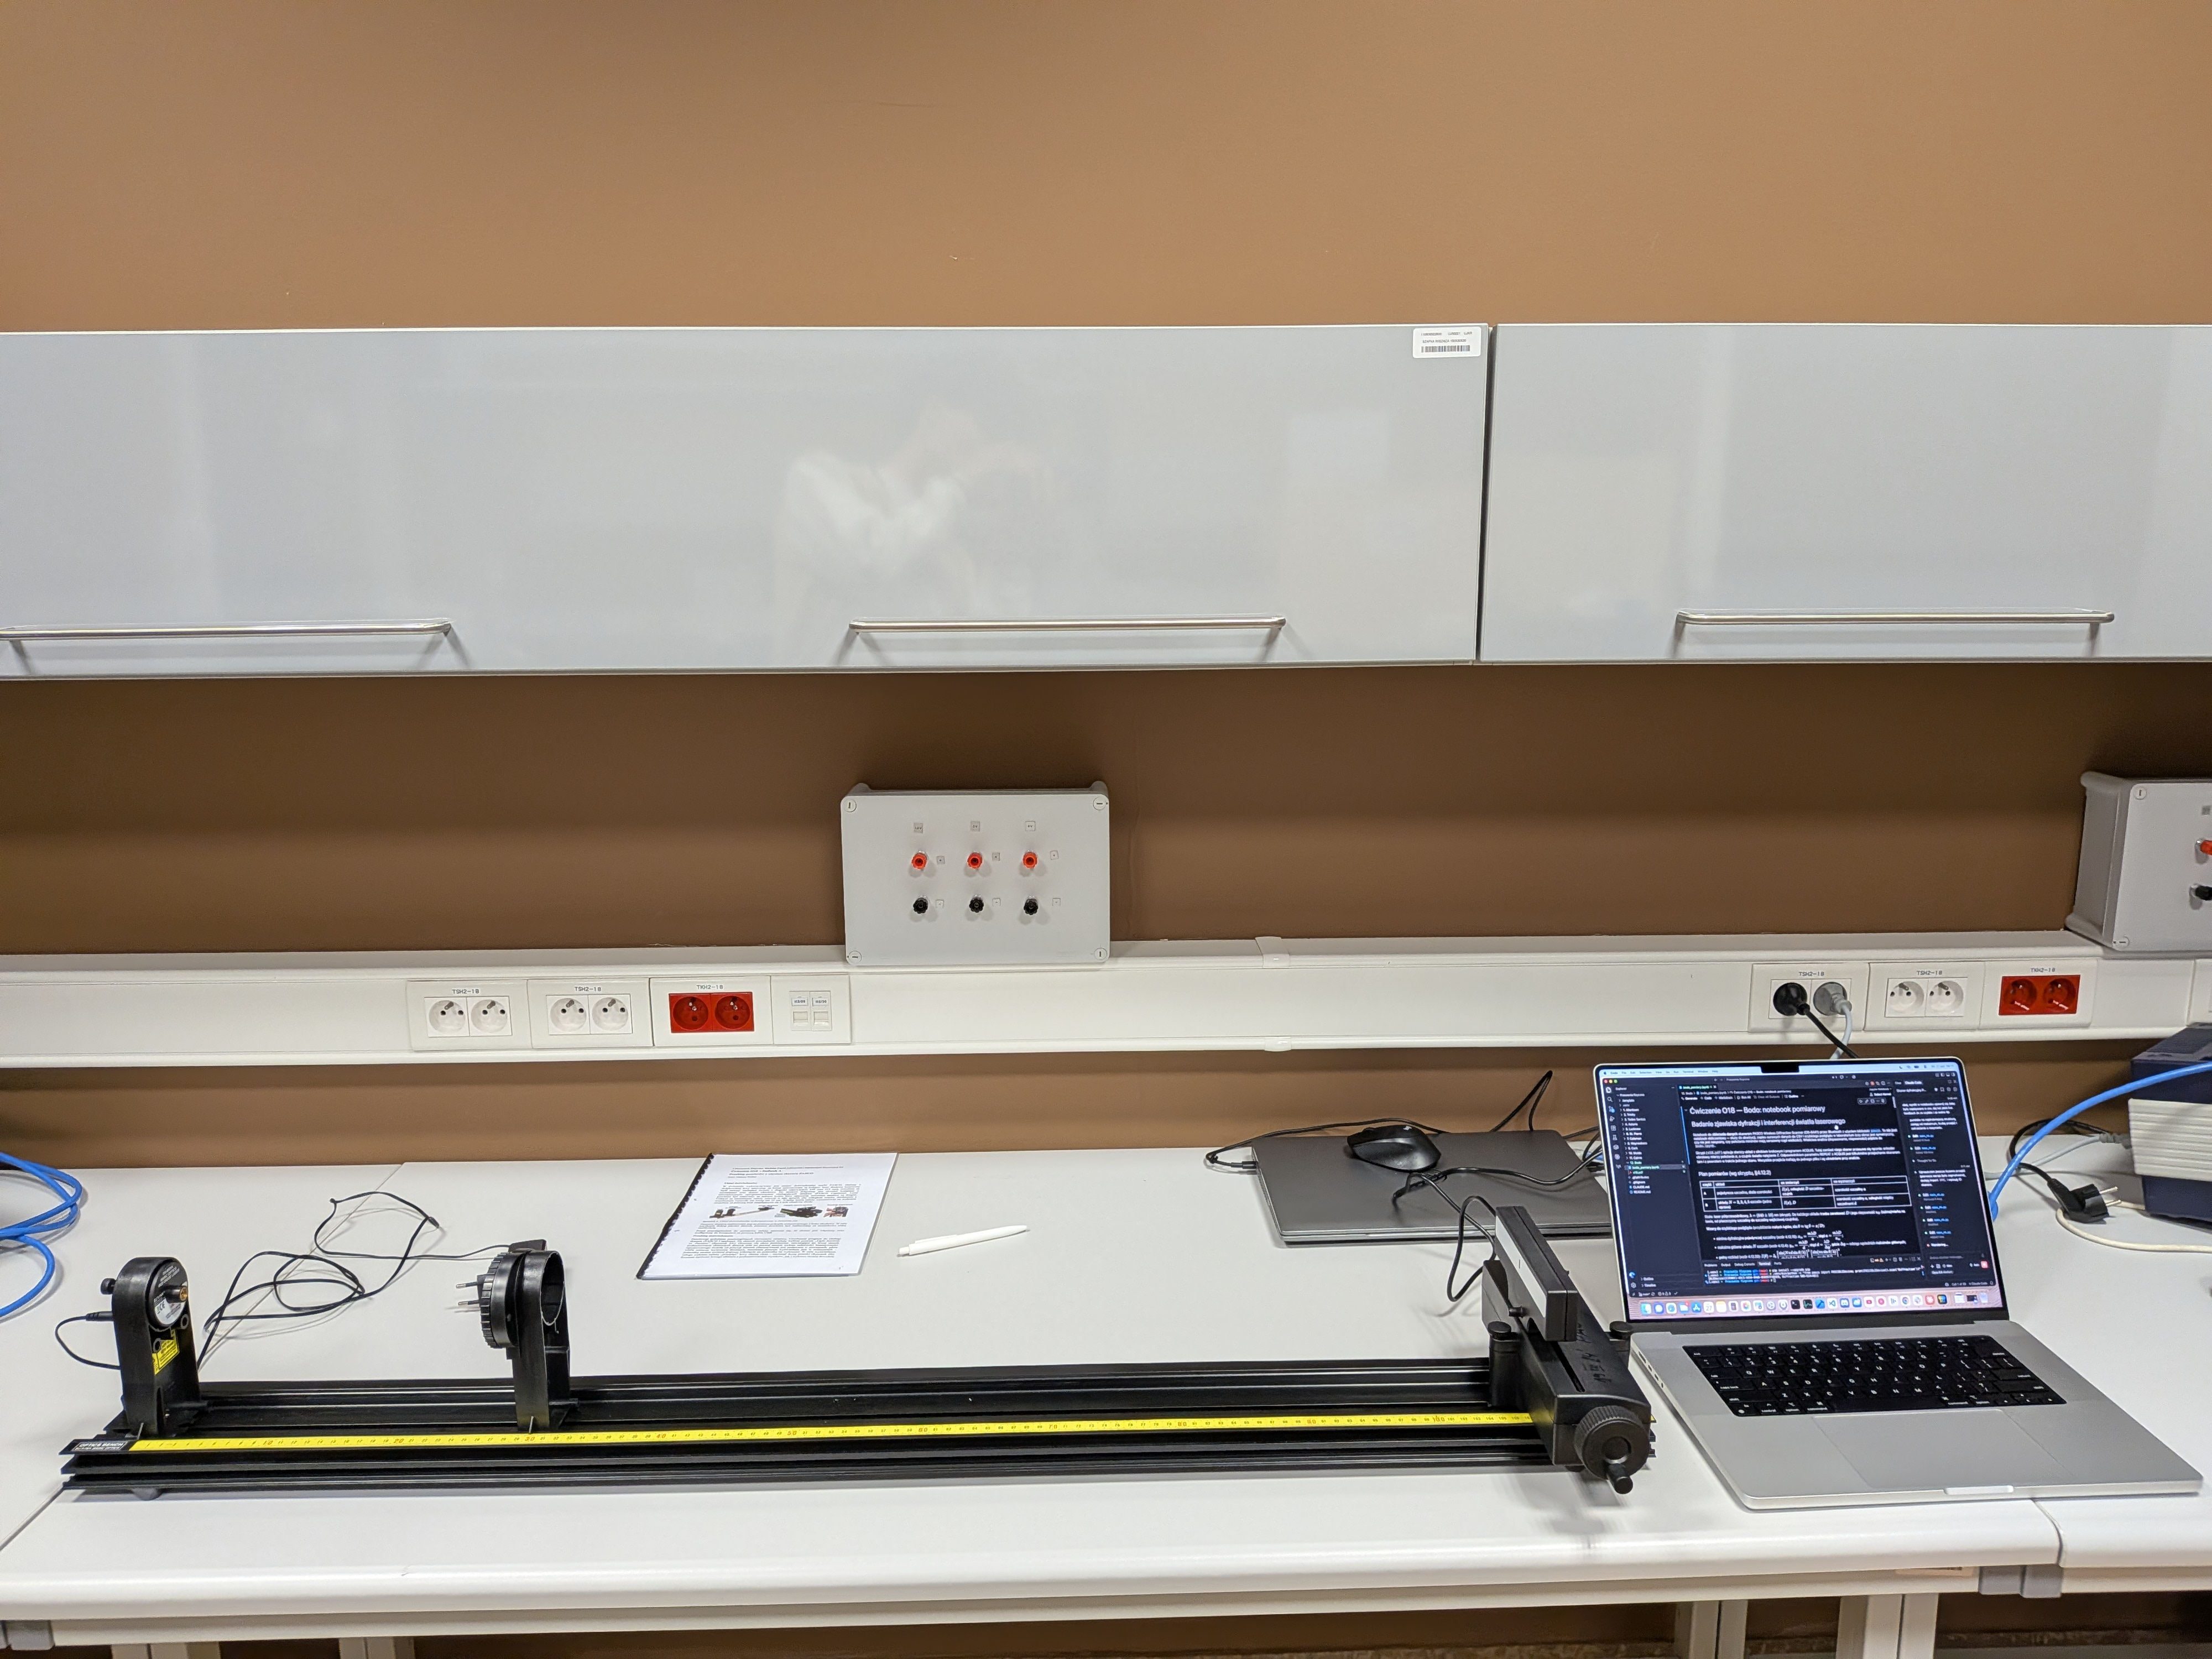
\includegraphics[width=0.85\textwidth]{schema.jpg}
    \caption{Układ pomiarowy: ława optyczna ze skalą, laser (z lewej), uchwyt z tarczą
             szczelin, skaner dyfrakcyjny z korbką (z prawej) i komputer rejestrujący dane.}
    \label{fig:setup}
\end{figure}

Wykorzystano:
\begin{itemize}
    \item lasery diodowe PASCO: czerwony, $\lambda = (650 \pm 5)$~nm, i zielony,
          $\lambda = (515 \pm 5)$~nm (wartości z tabliczek, niepewność przyjęta);
    \item tarczę szczelin PASCO OS-8442 z pojedynczymi szczelinami, parami szczelin
          i układami $N = 2$--$5$ szczelin (wymiary w podsekcji Przyjęte wartości);
    \item ławę optyczną ze skalą centymetrową; położenia uchwytów odczytywano
          z niepewnością $u_\text{poz} = 1$~cm;
    \item skaner dyfrakcyjny PASCO Wireless Diffraction Scanner OS-8441 z czujnikiem
          światła z wybieraną szczeliną wejściową (aperturą) i enkoderem obrotowym;
          według specyfikacji producenta zakres przesuwu głowicy wynosi 155~mm,
          rozdzielczość położenia $0{,}01$~mm, a apertura $0{,}1$--$1{,}5$~mm~\cite{pasco};
          biblioteka \texttt{pasco} przelicza impulsy enkodera na położenie jako
          $\SI{0.01}{\meter}$ na 2000 impulsów; natężenie w procentach zakresu czujnika;
    \item komputer z programem akwizycji w Pythonie; częstość odczytu przez Bluetooth
          wynosiła ok.\ 7 punktów na sekundę;
    \item ekran do wstępnego ustawienia obrazu.
\end{itemize}

Szczeliny ustawiono na 20~cm, a czujnik na 110~cm skali ławy, więc odległość
szczelina--detektor wynosiła $D = 900$~mm z niepewnością
$u_D = \sqrt{u_\text{poz}^2 + u_\text{poz}^2} \approx 14$~mm.

% -------------------------------------------
\section{Procedura pomiarowa}
% -------------------------------------------

Pomiary wykonano w dwóch sesjach: 27 października 2026 (laser czerwony: tło, pojedyncze
i podwójne szczeliny) oraz 3 listopada 2026 (laser czerwony: układy $N$ szczelin; laser
zielony: tło, pojedyncze i podwójne szczeliny, układ $N = 4$; na końcu laser czerwony:
zmiana odległości i apertury). Uchwytów szczelin i czujnika między sesjami nie przesuwano,
więc $D = 900$~mm jest wspólne dla obu laserów.

Po połączeniu ze skanerem wykonano test odczytu: przy przesuwaniu skanera ręką zmieniało się
$x$, a przy zasłonięciu lasera spadało $I$. Przed każdym pomiarem ustawiano na ekranie ostry,
symetryczny obraz dyfrakcyjny i usuwano ekran. Czułość czujnika dobierano tak, aby maksimum
centralne nie przekraczało ok.\ 95\,\% zakresu. W jednym z pomiarów, przy nasyceniu
czujnika, zmniejszono aperturę; nie zanotowano, którego pomiaru to dotyczyło.

Jeden pomiar to jeden przejazd skanera przez cały zakres przesuwu. Skaner ustawiano przy
jednym ograniczniku, uruchamiano rejestrację i przesuwano go korbką możliwie wolno i równo aż do
drugiego ogranicznika; tak wykonano wszystkie przejazdy.
Program zbierał punkty $(t, x, I)$ z częstością ok.\ 7 punktów na sekundę i na bieżąco
pokazywał prędkość przesuwu. Zalecana prędkość nie przekraczała $v_\text{max} = f s/8$,
gdzie $f$ --- częstość odczytu, a $s$ --- szerokość najdrobniejszej struktury obrazu
przewidziana dla nominalnych wymiarów szczelin, $\lambda D/2a$ dla pojedynczej szczeliny
i $\lambda D/Nd$ dla $N$ szczelin. Zapewnia to co najmniej 8 punktów na strukturę.
Program ostrzegał też o nasyceniu ($I > 95\,\%$). Pomiar kończył się, gdy skaner po
przejechaniu co najmniej 10~mm cofnął się o ponad 1~mm (po dojściu do drugiego ogranicznika
skaner cofano). Do pliku zapisywano tylko przejazd --- od ostatniego zawrotu przy ustawianiu
do najdalszego punktu. Ostatni zawrót mógł wypaść kilka milimetrów od ogranicznika, więc
zapisany przejazd bywa nieco krótszy od pełnego przesuwu (podsekcja~\ref{sec:calib}). Parametry układu
($\lambda$, położenia uchwytów, $D$, nominalne $a$ i $d$) trafiały do rejestru pomiarów.

Każdy układ szczelin mierzono trzema przejazdami, jeden po drugim, na przemian w obu
kierunkach. Przejazdy przerwane albo z nasyceniem czujnika powtarzano pod tą samą nazwą
pliku; w analizie użyto ostatniego zapisu.

\subsection{Pomiar tła}

Przy zasłoniętym laserze wykonano jeden przejazd przez całą oś, w sesji każdego lasera
osobno.

\subsection{Pojedyncza szczelina}

Laserem czerwonym zmierzono rozkłady dla szczelin $a = 0{,}02;\ 0{,}04;\ 0{,}08;\ 0{,}16$~mm.
Pierwsze przejazdy dla $a = 0{,}16$~mm nasyciły czujnik ($I \approx 100\,\%$), więc po
zmianie ustawień powtórzono je. Laserem zielonym zmierzono szczeliny $a = 0{,}08$
i $0{,}04$~mm, w tej kolejności.

\subsection{Dwie szczeliny}

Laserem czerwonym zmierzono wszystkie cztery pary, $a \in \{0{,}04;\ 0{,}08\}$~mm
i $d \in \{0{,}25;\ 0{,}50\}$~mm (pierwszy przejazd dla $a = 0{,}08$~mm, $d = 0{,}25$~mm
nasycił czujnik i został powtórzony), a zielonym --- pary o $a = 0{,}08$~mm
i $d = 0{,}25$ oraz $0{,}50$~mm. Prążki interferencyjne są tu najdrobniejszą strukturą
obrazu, więc przejazdy były najwolniejsze ($\bar v \approx 0{,}4$--$1{,}6$~mm/s).

\subsection{Układy $N$ szczelin}

Laserem czerwonym zmierzono układy $N = 2, 3, 4, 5$ szczelin ($a = 0{,}04$~mm,
$d = 0{,}125$~mm), a zielonym --- układ $N = 4$. Na ekranie obserwowano, jak ze wzrostem
$N$ zmieniają się szerokość i natężenie maksimów głównych oraz liczba maksimów pobocznych.

\subsection{Zmiana odległości szczelina--detektor}

Dla szczeliny $a = 0{,}02$~mm i lasera czerwonego przesunięto uchwyt ze szczelinami
na 10, 60 i 70~cm skali ławy, przy czujniku nadal na 110~cm ($D = 1000$, $500$ i $400$~mm),
i w każdym położeniu wykonano jeden przejazd. Ten układ wybrano, bo skanuje się
najszybciej: szeroki obraz pozwala na przesuw ok.\ 5--9~mm/s. Pomiarem odniesienia
dla $D = 900$~mm jest seria dla tej samej szczeliny z części Pojedyncza szczelina.

\subsection{Zmiana apertury czujnika}

Laserem czerwonym, przy $D = 900$~mm, wykonano po jednym przejeździe z aperturami
czujnika $0{,}1$ i $1{,}5$~mm, czyli najwęższą i najszerszą aperturą skanera~\cite{pasco}.
Oznaczenie szerszej apertury zasłaniała naklejka inwentaryzacyjna i w notatkach zapisano ją
jako $0{,}7$ (siódma pozycja tarczy). Takiej apertury skaner nie ma, a stosunek natężeń
(Opracowanie) wskazuje na $1{,}5$~mm. Pomiar zaplanowano dla szczeliny $a = 0{,}04$~mm, ale
w uchwycie została szczelina $a = 0{,}02$~mm z poprzedniej części, co wynika z szerokości
zarejestrowanego obrazu. Pomiarem odniesienia jest więc seria dla $a = 0{,}02$~mm.
Apertury używanej w pozostałych pomiarach nie zanotowano.

% -------------------------------------------
\section{Wyniki pomiarów}
% -------------------------------------------

Położenie $x$ zapisane przez program (przelicznik biblioteki \texttt{pasco}: $\SI{0.01}{\meter}$
na 2000 impulsów) zaniża rzeczywiste przesunięcie. Pełny przesuw głowicy, 155~mm według
specyfikacji~\cite{pasco}, zapisywał się jako najwyżej $85{,}8$~mm. Dlatego wszystkie położenia
w tabelach i na wykresach pomnożono przez czynnik kalibracji
$K_x = 155/85{,}78 = 1{,}807 \pm 0{,}016$; jego wyznaczenie opisano w
podsekcji~\ref{sec:calib}. Natężenie $I$ podano
w procentach zakresu czujnika. Niepewności pojedynczego odczytu $I$ nie wyznaczono
bezpośrednio --- rozrzut tła (podsekcja Pomiar tła) obejmuje tylko szum czujnika,
a nie drgania wiązki --- dlatego oszacowano ją dopiero z residuów dopasowań. Na wykresach
nie zaznaczono słupków błędów; niepewność położenia jest mniejsza od rozmiaru punktów.

Wszystkie przejazdy zestawiono w Tabelach~\ref{tab:scans_red} i~\ref{tab:scans_green}.
Każdy plik zawiera kilkaset do kilku tysięcy punktów $(t, x, I)$, więc dane surowe
przedstawiono na wykresach --- dla każdego układu pierwszy przejazd, z osią $x$ przesuniętą
o środek obrazu $C$ (wyznaczony z dopasowania w Opracowaniu, tylko dla czytelności).

\begin{table}[H]
    \centering
    \caption{Zestawienie przejazdów, laser czerwony: kierunek ruchu skanera ($\rightarrow$ --- rosnące $x$),
             liczba punktów $n$, zakres położeń (po kalibracji), czas przejazdu $T$, średnia prędkość
             $\bar v = (x_\text{max} - x_\text{min})/T$ i największe natężenie $I_\text{max}$.}
    \label{tab:scans_red}
    \footnotesize
    \begin{tabular}{l c S[table-format=4.0] S[table-format=-3.1] S[table-format=-3.1]
                    S[table-format=3.0] S[table-format=1.2] S[table-format=2.2]}
        \toprule
        układ & kier. & {$n$} & {$x_\text{min}$ [mm]} & {$x_\text{max}$ [mm]} & {$T$ [s]}
              & {$\bar v$ [mm/s]} & {$I_\text{max}$ [\%]} \\
        \midrule
        tło & $\rightarrow$ & 1500 & -0.2 & 152.8 & 215 & 0.71 & 0.73 \\
        1 szczelina, $a = 0{,}02$ & $\rightarrow$ & 177 & -64.2 & 86.7 & 25 & 6.00 & 2.30 \\
        1 szczelina, $a = 0{,}02$ & $\leftarrow$ & 126 & -64.5 & 80.5 & 18 & 8.13 & 2.24 \\
        1 szczelina, $a = 0{,}02$ & $\rightarrow$ & 124 & -57.4 & 87.7 & 17 & 8.37 & 2.23 \\
        1 szczelina, $a = 0{,}04$ & $\leftarrow$ & 383 & -59.9 & 90.5 & 54 & 2.78 & 7.71 \\
        1 szczelina, $a = 0{,}04$ & $\rightarrow$ & 245 & -55.8 & 91.6 & 34 & 4.29 & 9.17 \\
        1 szczelina, $a = 0{,}04$ & $\leftarrow$ & 219 & -62.0 & 87.8 & 31 & 4.83 & 9.99 \\
        1 szczelina, $a = 0{,}08$ & $\leftarrow$ & 358 & -73.8 & 67.0 & 51 & 2.76 & 29.92 \\
        1 szczelina, $a = 0{,}08$ & $\rightarrow$ & 413 & -69.7 & 78.0 & 59 & 2.52 & 33.62 \\
        1 szczelina, $a = 0{,}08$ & $\leftarrow$ & 381 & -73.0 & 74.6 & 54 & 2.73 & 35.25 \\
        1 szczelina, $a = 0{,}16$ & $\rightarrow$ & 772 & -9.3 & 141.6 & 109 & 1.39 & 47.79 \\
        1 szczelina, $a = 0{,}16$ & $\leftarrow$ & 860 & -10.9 & 139.1 & 122 & 1.23 & 50.76 \\
        1 szczelina, $a = 0{,}16$ & $\rightarrow$ & 615 & -6.4 & 141.7 & 87 & 1.70 & 52.18 \\
        2 szczeliny, $a = 0{,}04$, $d = 0{,}25$ & $\leftarrow$ & 1309 & -8.5 & 143.0 & 185 & 0.82 & 37.70 \\
        2 szczeliny, $a = 0{,}04$, $d = 0{,}25$ & $\rightarrow$ & 673 & -5.3 & 141.9 & 95 & 1.55 & 36.70 \\
        2 szczeliny, $a = 0{,}04$, $d = 0{,}25$ & $\leftarrow$ & 818 & -9.2 & 139.2 & 115 & 1.29 & 37.95 \\
        2 szczeliny, $a = 0{,}04$, $d = 0{,}50$ & $\rightarrow$ & 2479 & -5.6 & 147.1 & 354 & 0.43 & 42.70 \\
        2 szczeliny, $a = 0{,}04$, $d = 0{,}50$ & $\leftarrow$ & 2053 & -5.6 & 145.2 & 292 & 0.52 & 45.77 \\
        2 szczeliny, $a = 0{,}04$, $d = 0{,}50$ & $\rightarrow$ & 2669 & -3.1 & 145.1 & 380 & 0.39 & 47.54 \\
        2 szczeliny, $a = 0{,}08$, $d = 0{,}25$ & $\rightarrow$ & 1482 & -51.5 & 100.6 & 211 & 0.72 & 59.25 \\
        2 szczeliny, $a = 0{,}08$, $d = 0{,}25$ & $\leftarrow$ & 935 & -51.8 & 98.3 & 133 & 1.13 & 57.90 \\
        2 szczeliny, $a = 0{,}08$, $d = 0{,}25$ & $\rightarrow$ & 666 & -48.8 & 100.9 & 95 & 1.58 & 60.02 \\
        2 szczeliny, $a = 0{,}08$, $d = 0{,}50$ & $\leftarrow$ & 3030 & -50.9 & 102.4 & 434 & 0.35 & 60.34 \\
        2 szczeliny, $a = 0{,}08$, $d = 0{,}50$ & $\rightarrow$ & 2049 & -48.8 & 103.0 & 293 & 0.52 & 57.99 \\
        2 szczeliny, $a = 0{,}08$, $d = 0{,}50$ & $\leftarrow$ & 2127 & -48.8 & 100.6 & 303 & 0.49 & 56.76 \\
        $N = 2$ & $\rightarrow$ & 521 & -170.5 & -20.9 & 74 & 2.02 & 8.00 \\
        $N = 2$ & $\leftarrow$ & 527 & -174.5 & -25.4 & 75 & 1.99 & 10.67 \\
        $N = 2$ & $\rightarrow$ & 674 & -171.5 & -22.0 & 96 & 1.56 & 11.72 \\
        $N = 3$ & $\rightarrow$ & 1066 & -176.9 & -25.8 & 152 & 0.99 & 25.66 \\
        $N = 3$ & $\leftarrow$ & 1197 & -176.7 & -28.0 & 170 & 0.88 & 20.33 \\
        $N = 3$ & $\rightarrow$ & 1470 & -174.0 & -23.3 & 209 & 0.72 & 25.06 \\
        $N = 4$ & $\leftarrow$ & 1802 & -174.3 & -22.6 & 258 & 0.59 & 49.43 \\
        $N = 4$ & $\rightarrow$ & 1536 & -172.2 & -21.1 & 218 & 0.69 & 47.52 \\
        $N = 4$ & $\leftarrow$ & 1633 & -173.1 & -23.3 & 233 & 0.64 & 39.49 \\
        $N = 5$ & $\rightarrow$ & 2085 & -0.1 & 151.6 & 295 & 0.51 & 71.63 \\
        $N = 5$ & $\leftarrow$ & 1469 & -0.3 & 149.5 & 208 & 0.72 & 71.37 \\
        $N = 5$ & $\rightarrow$ & 1828 & 1.8 & 151.3 & 259 & 0.58 & 69.48 \\
        1 szczelina, $a = 0{,}02$, $D = 1000$ & $\rightarrow$ & 190 & -70.4 & 83.9 & 27 & 5.70 & 1.20 \\
        1 szczelina, $a = 0{,}02$, $D = 500$ & $\leftarrow$ & 166 & -68.9 & 86.1 & 24 & 6.52 & 1.47 \\
        1 szczelina, $a = 0{,}02$, $D = 400$ & $\rightarrow$ & 213 & -72.8 & 80.4 & 30 & 5.04 & 1.95 \\
        1 szczelina, $a = 0{,}02$, apertura 0,1 & $\leftarrow$ & 645 & -67.5 & 83.1 & 91 & 1.65 & 1.34 \\
        1 szczelina, $a = 0{,}02$, apertura 1,5 & $\rightarrow$ & 815 & -57.3 & 88.0 & 116 & 1.25 & 12.04 \\
        \bottomrule
    \end{tabular}
\end{table}

\begin{table}[H]
    \centering
    \caption{Zestawienie przejazdów, laser zielony: kierunek ruchu skanera ($\rightarrow$ --- rosnące $x$),
             liczba punktów $n$, zakres położeń (po kalibracji), czas przejazdu $T$, średnia prędkość
             $\bar v = (x_\text{max} - x_\text{min})/T$ i największe natężenie $I_\text{max}$.}
    \label{tab:scans_green}
    \footnotesize
    \begin{tabular}{l c S[table-format=4.0] S[table-format=-3.1] S[table-format=-3.1]
                    S[table-format=3.0] S[table-format=1.2] S[table-format=2.2]}
        \toprule
        układ & kier. & {$n$} & {$x_\text{min}$ [mm]} & {$x_\text{max}$ [mm]} & {$T$ [s]}
              & {$\bar v$ [mm/s]} & {$I_\text{max}$ [\%]} \\
        \midrule
        tło & $\leftarrow$ & 1620 & -88.8 & 63.6 & 231 & 0.66 & 0.60 \\
        1 szczelina, $a = 0{,}04$ & $\leftarrow$ & 447 & -102.2 & 48.4 & 64 & 2.37 & 7.13 \\
        1 szczelina, $a = 0{,}04$ & $\rightarrow$ & 580 & -99.5 & 49.4 & 82 & 1.82 & 7.00 \\
        1 szczelina, $a = 0{,}04$ & $\leftarrow$ & 680 & -102.3 & 46.6 & 97 & 1.54 & 6.78 \\
        1 szczelina, $a = 0{,}08$ & $\rightarrow$ & 781 & -90.2 & 61.9 & 111 & 1.37 & 24.37 \\
        1 szczelina, $a = 0{,}08$ & $\leftarrow$ & 372 & -89.9 & 59.2 & 53 & 2.83 & 24.84 \\
        1 szczelina, $a = 0{,}08$ & $\rightarrow$ & 790 & -87.2 & 64.3 & 112 & 1.35 & 25.08 \\
        2 szczeliny, $a = 0{,}08$, $d = 0{,}25$ & $\rightarrow$ & 1513 & -103.7 & 49.0 & 215 & 0.71 & 77.71 \\
        2 szczeliny, $a = 0{,}08$, $d = 0{,}25$ & $\leftarrow$ & 1780 & -102.2 & 46.4 & 252 & 0.59 & 76.92 \\
        2 szczeliny, $a = 0{,}08$, $d = 0{,}25$ & $\rightarrow$ & 1285 & -100.1 & 51.1 & 183 & 0.83 & 79.51 \\
        2 szczeliny, $a = 0{,}08$, $d = 0{,}50$ & $\leftarrow$ & 2289 & -97.9 & 53.4 & 326 & 0.46 & 78.27 \\
        2 szczeliny, $a = 0{,}08$, $d = 0{,}50$ & $\rightarrow$ & 1794 & -95.5 & 54.0 & 255 & 0.59 & 80.98 \\
        2 szczeliny, $a = 0{,}08$, $d = 0{,}50$ & $\leftarrow$ & 1441 & -98.3 & 51.7 & 205 & 0.73 & 80.17 \\
        $N = 4$ & $\rightarrow$ & 1600 & -100.8 & 50.5 & 227 & 0.67 & 94.31 \\
        $N = 4$ & $\leftarrow$ & 1984 & -102.2 & 48.0 & 282 & 0.53 & 94.07 \\
        $N = 4$ & $\rightarrow$ & 2182 & -100.2 & 48.4 & 309 & 0.48 & 90.93 \\
        \bottomrule
    \end{tabular}
\end{table}

\subsection{Pomiar tła}

Średnie natężenie tła wyniosło $I_\text{tło} = 0{,}624\,\%$ przy odchyleniu standardowym
$\sigma = 0{,}019\,\%$ (laser czerwony, 1500 punktów) oraz $I_\text{tło} = 0{,}561\,\%$,
$\sigma = 0{,}008\,\%$ (laser zielony, 1620 punktów).

\subsection{Pojedyncza szczelina}

Zarejestrowane rozkłady natężenia przedstawiono na Rysunkach~\ref{fig:single_red_raw}
i~\ref{fig:single_green_raw}.

\begin{figure}[H]
    \centering
    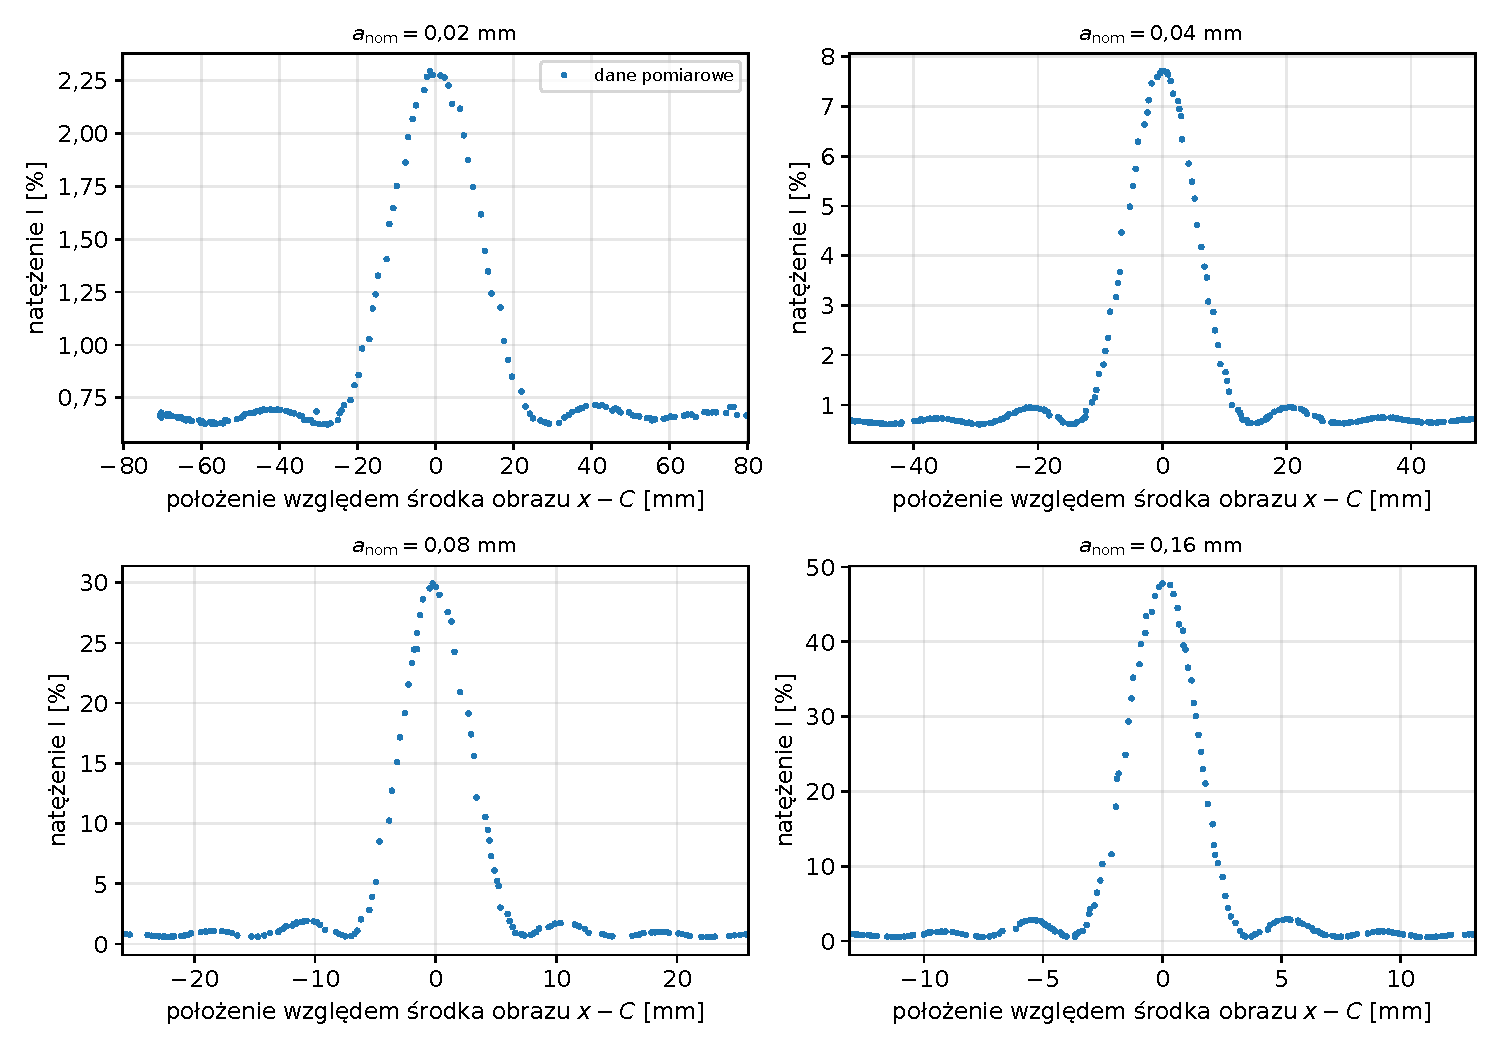
\includegraphics[width=0.9\textwidth]{single_slit_red_raw.pdf}
    \caption{Rozkład natężenia za pojedynczą szczeliną, laser czerwony, $D = 900$~mm,
             pierwszy przejazd dla każdej szerokości $a_\text{nom}$.}
    \label{fig:single_red_raw}
\end{figure}

\begin{figure}[H]
    \centering
    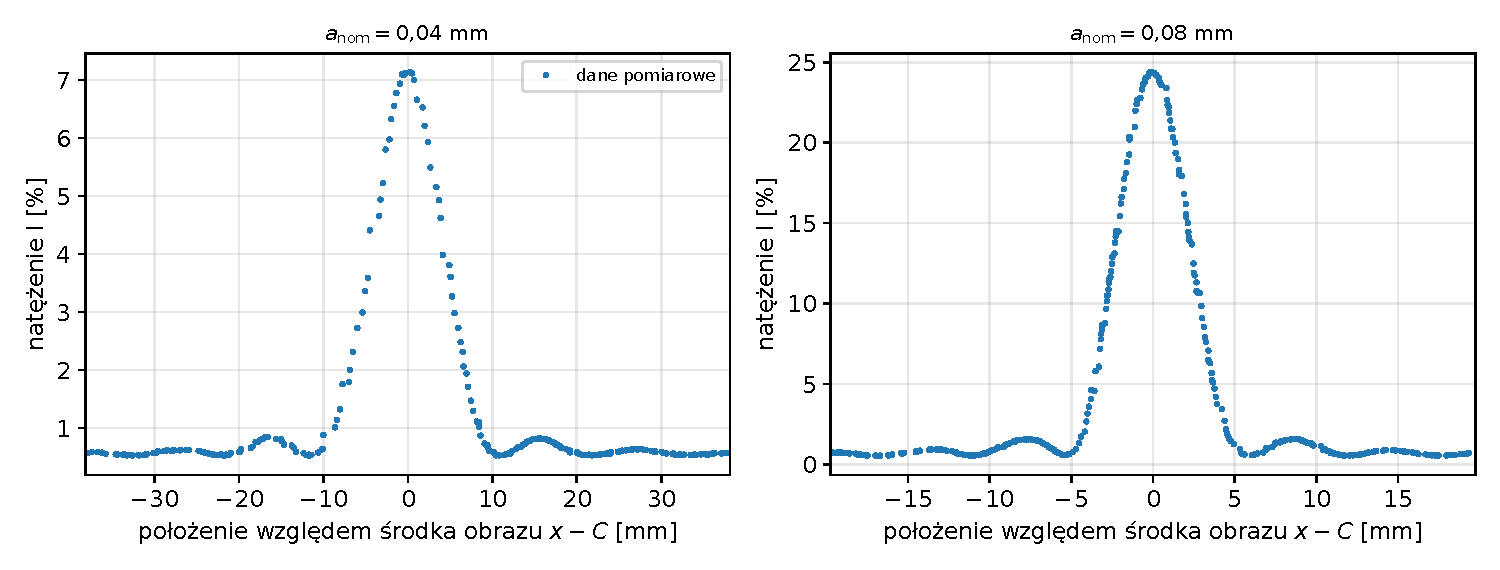
\includegraphics[width=0.9\textwidth]{single_slit_green_raw.pdf}
    \caption{Rozkład natężenia za pojedynczą szczeliną, laser zielony, $D = 900$~mm,
             pierwszy przejazd.}
    \label{fig:single_green_raw}
\end{figure}

\subsection{Dwie szczeliny}

Rozkłady dla par szczelin przedstawiono na Rysunkach~\ref{fig:double_red_raw}
i~\ref{fig:double_green_raw}.

\begin{figure}[H]
    \centering
    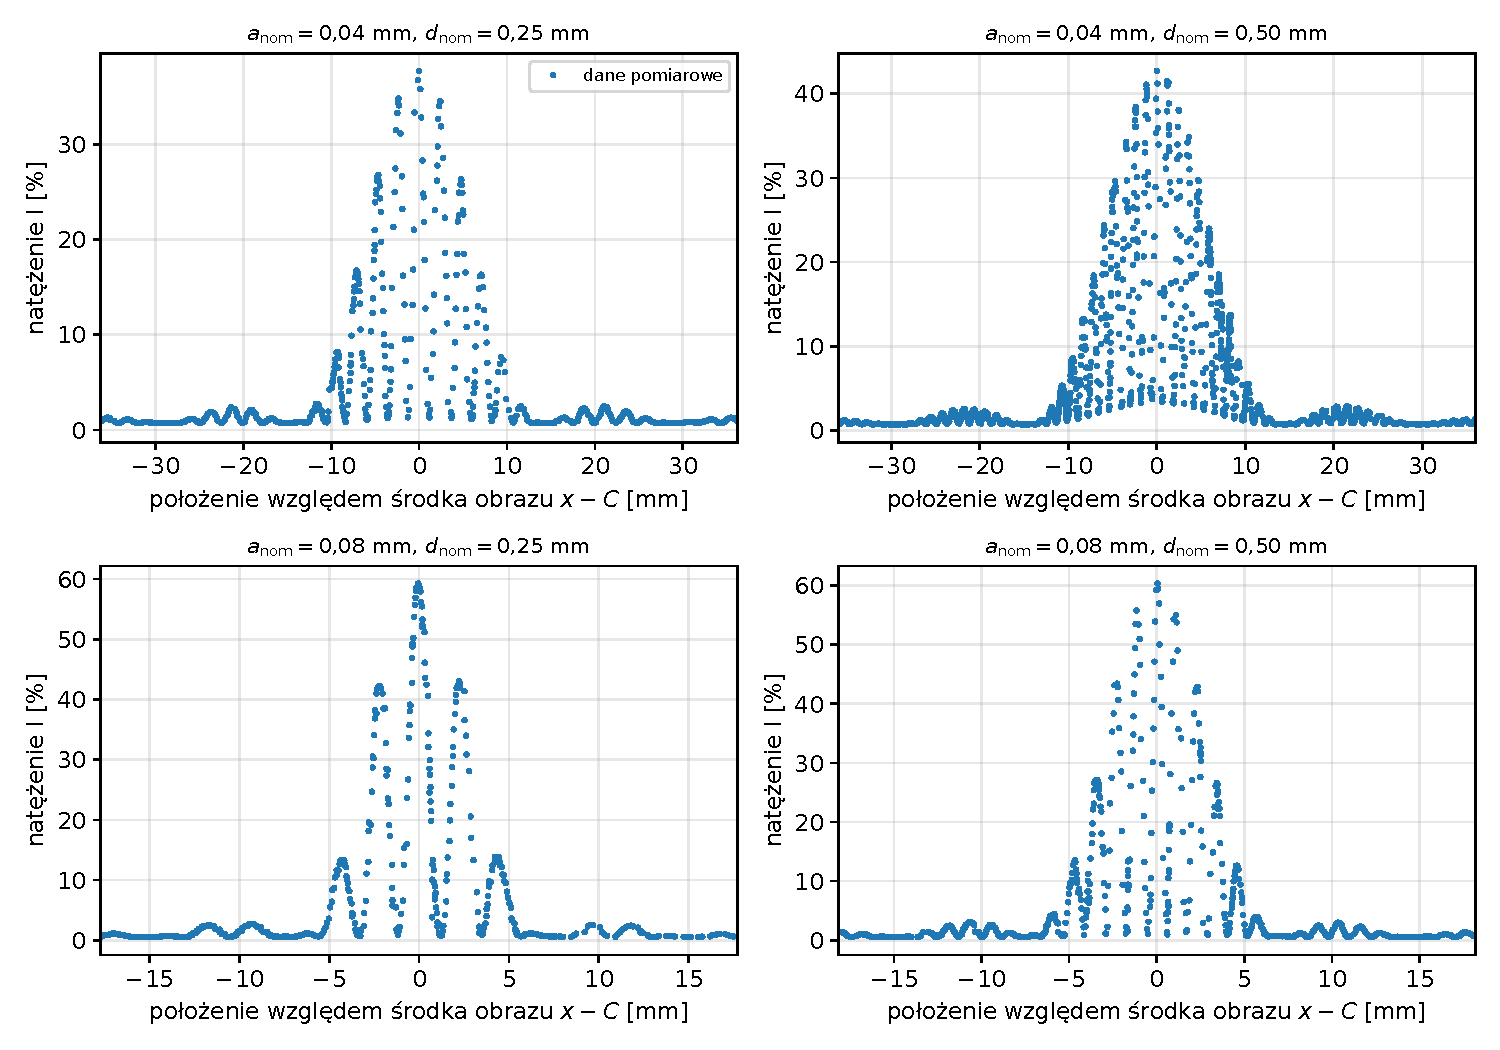
\includegraphics[width=0.9\textwidth]{double_slit_red_raw.pdf}
    \caption{Rozkład natężenia za dwiema szczelinami, laser czerwony, $D = 900$~mm,
             pierwszy przejazd dla każdej pary $(a_\text{nom}, d_\text{nom})$.}
    \label{fig:double_red_raw}
\end{figure}

\begin{figure}[H]
    \centering
    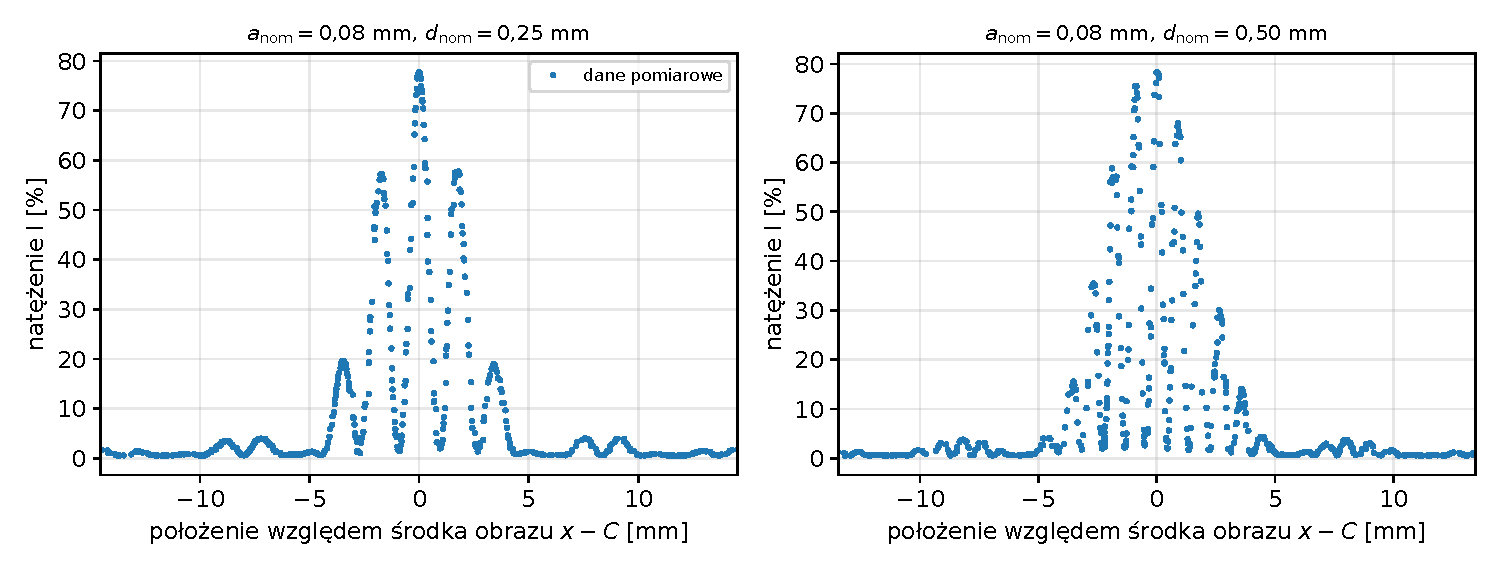
\includegraphics[width=0.9\textwidth]{double_slit_green_raw.pdf}
    \caption{Rozkład natężenia za dwiema szczelinami ($a_\text{nom} = 0{,}08$~mm),
             laser zielony, $D = 900$~mm, pierwszy przejazd.}
    \label{fig:double_green_raw}
\end{figure}

\subsection{Układy $N$ szczelin}

Rozkłady dla układów $N$ szczelin przedstawiono na Rysunkach~\ref{fig:multi_red_raw}
i~\ref{fig:multi_green_raw}.

\begin{figure}[H]
    \centering
    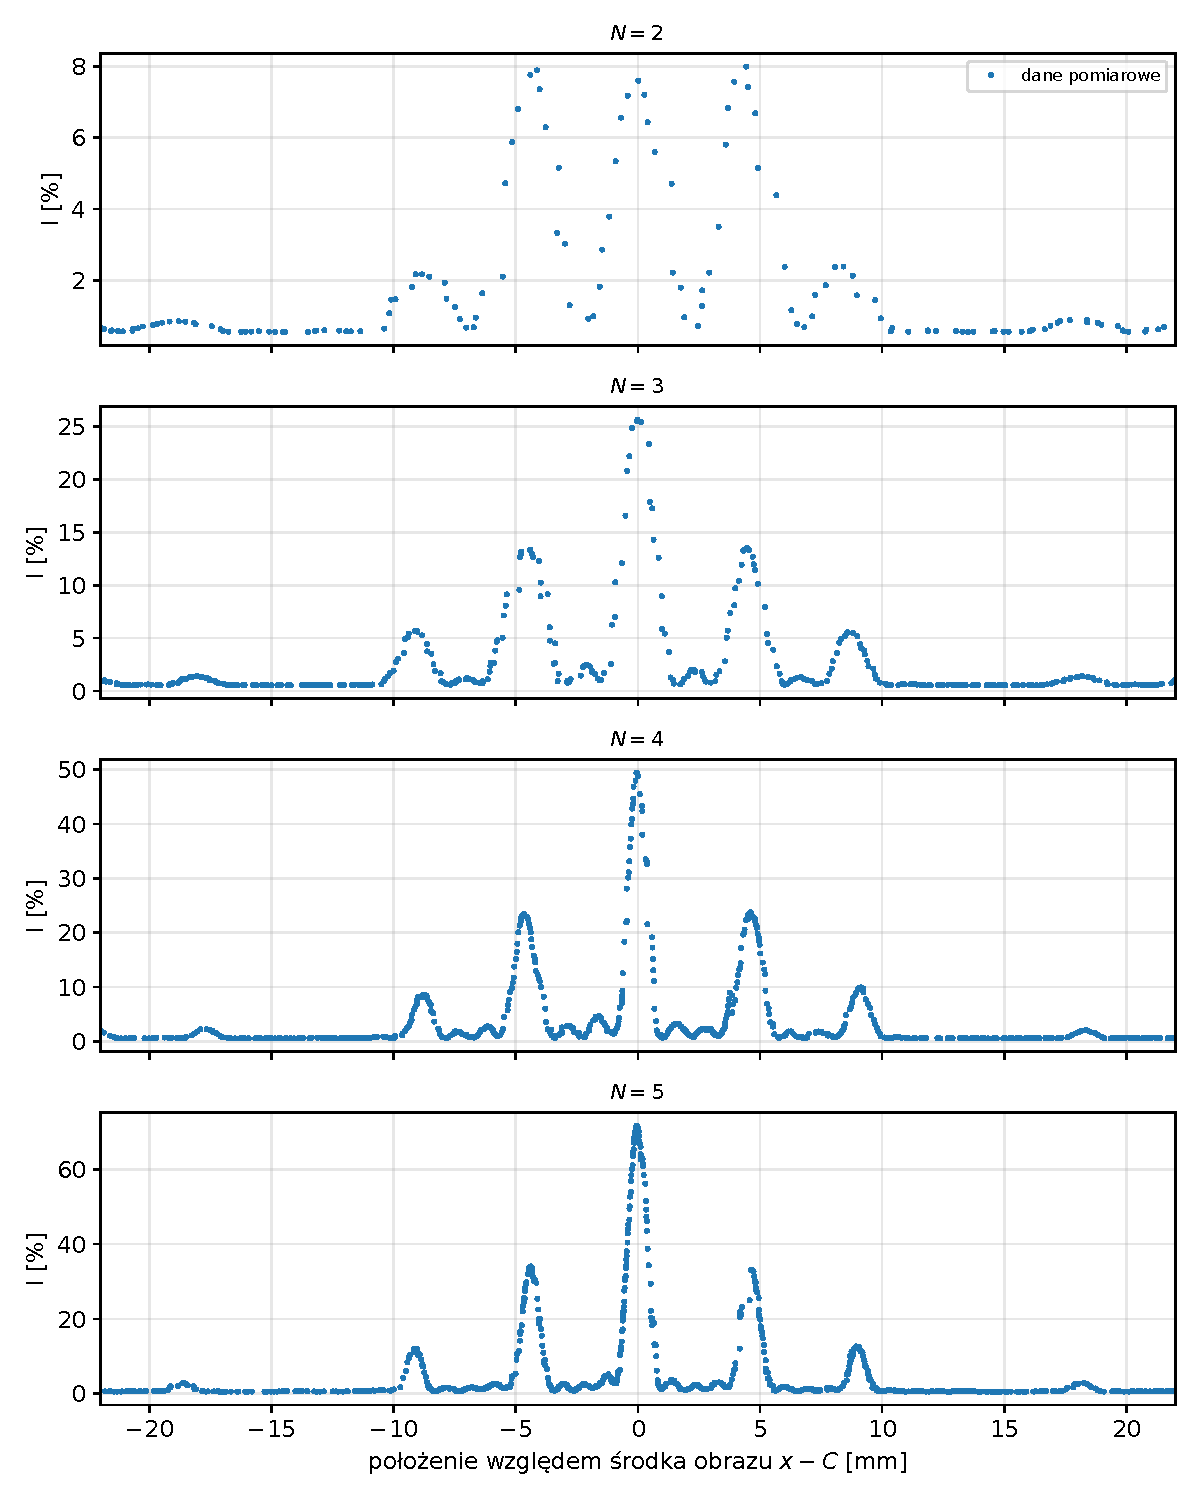
\includegraphics[width=0.75\textwidth]{multi_slit_red_raw.pdf}
    \caption{Rozkład natężenia dla układów $N = 2$--$5$ szczelin ($a_\text{nom} = 0{,}04$~mm,
             $d_\text{nom} = 0{,}125$~mm), laser czerwony, $D = 900$~mm, pierwszy przejazd;
             zakres $|x - C| < 22$~mm.}
    \label{fig:multi_red_raw}
\end{figure}

\begin{figure}[H]
    \centering
    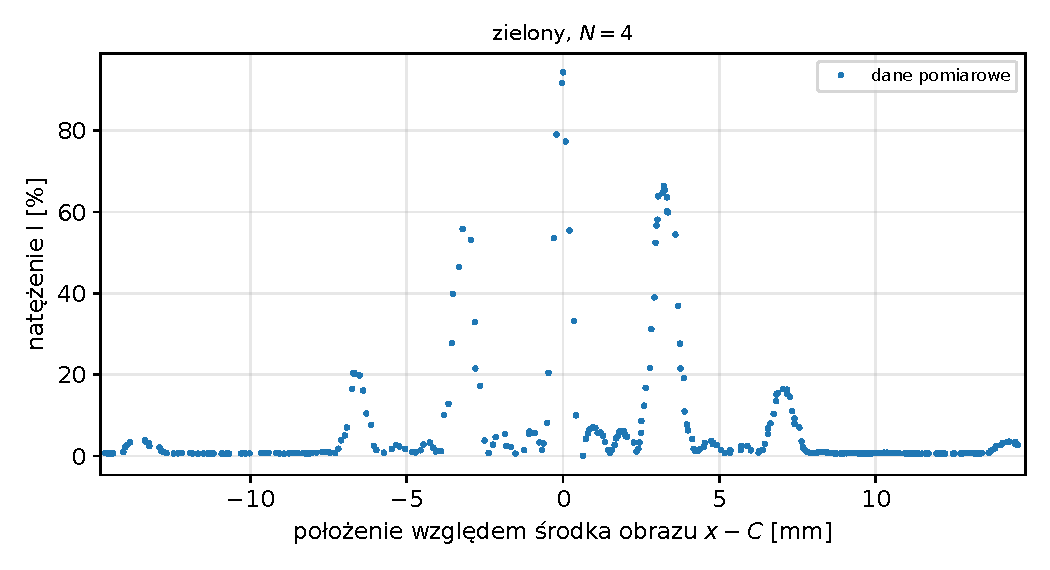
\includegraphics[width=0.6\textwidth]{multi_slit_green_raw.pdf}
    \caption{Rozkład natężenia dla układu $N = 4$ szczelin, laser zielony, $D = 900$~mm,
             pierwszy przejazd.}
    \label{fig:multi_green_raw}
\end{figure}

\subsection{Zmiana odległości szczelina--detektor}

Rozkłady dla szczeliny $a_\text{nom} = 0{,}02$~mm przy czterech odległościach $D$
przedstawiono na Rysunku~\ref{fig:distance_raw}. Szerokość maksimum centralnego rośnie
wraz z $D$. Przy $D = 400$, $500$ i $1000$~mm (sesja 3 listopada) maksimum centralne jest
rozdwojone, czego nie ma w pomiarze dla $D = 900$~mm z 27 października.

\begin{figure}[H]
    \centering
    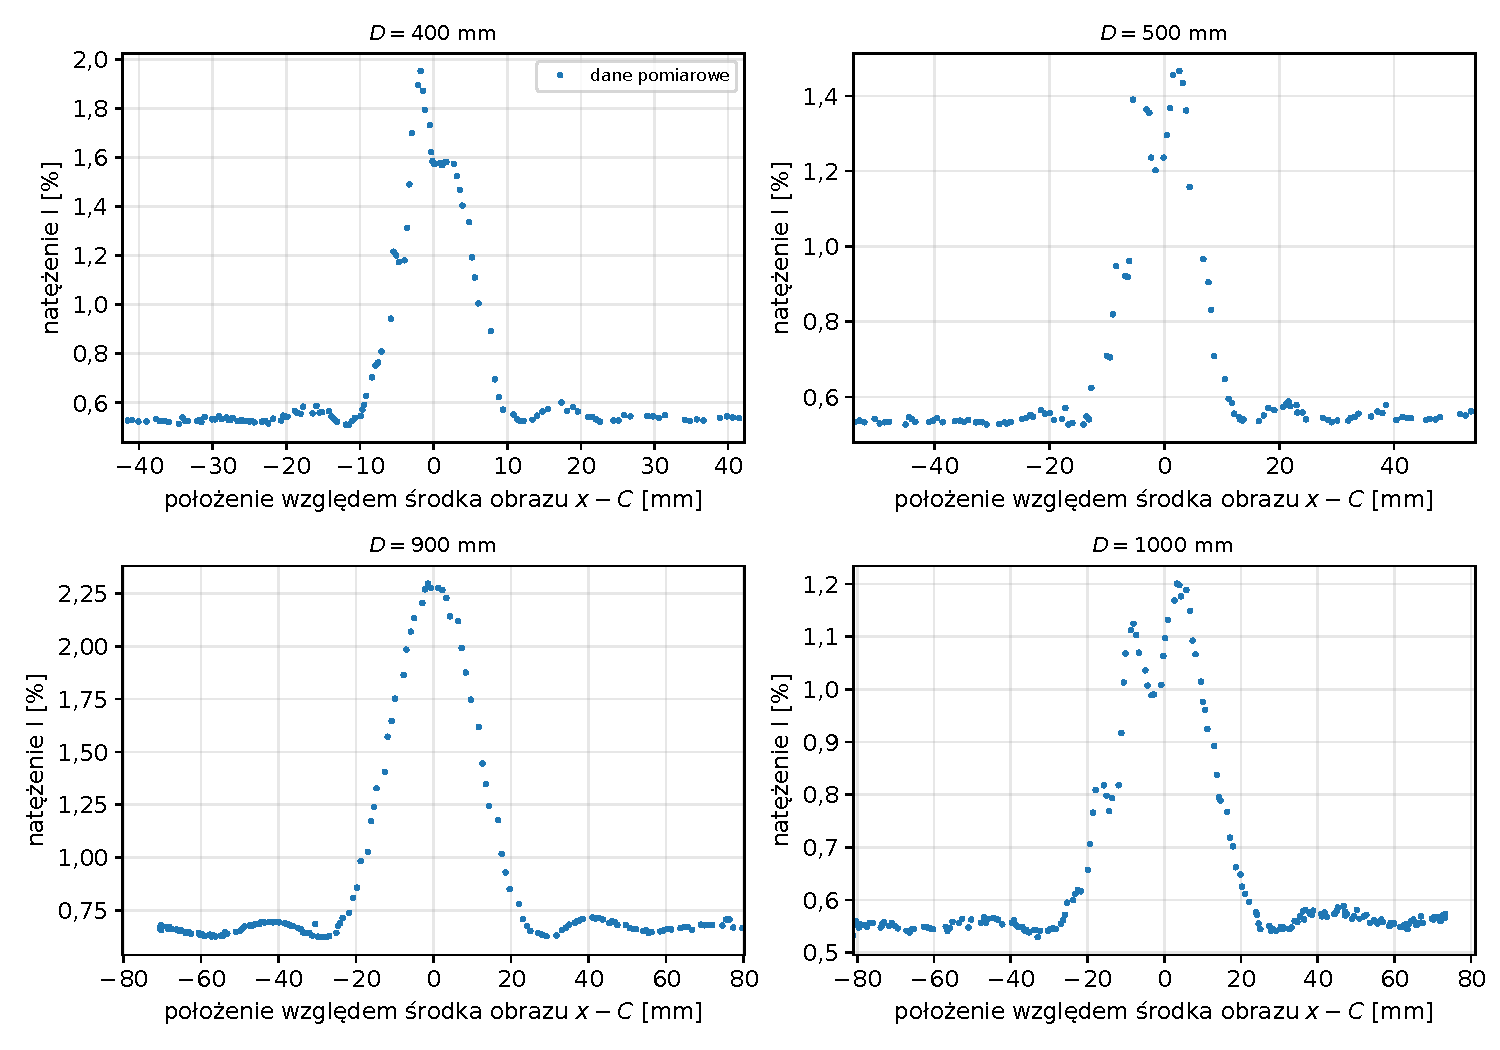
\includegraphics[width=0.9\textwidth]{distance_raw.pdf}
    \caption{Rozkład natężenia za szczeliną $a_\text{nom} = 0{,}02$~mm, laser czerwony,
             dla różnych odległości szczelina--detektor $D$ (dla $D = 900$~mm pierwszy
             przejazd serii z części Pojedyncza szczelina).}
    \label{fig:distance_raw}
\end{figure}

\subsection{Zmiana apertury czujnika}

Rozkłady dla dwóch apertur porównano z pomiarem przy aperturze zwykłej na
Rysunku~\ref{fig:aperture_raw}. Przy aperturze $1{,}5$~mm maksimum jest wyraźnie wyższe niż
przy zwykłej ($I_\text{max} = 12{,}0\,\%$ wobec $2{,}3\,\%$), a przy aperturze $0{,}1$~mm ---
niższe ($1{,}3\,\%$, ok.\ 2 razy więcej niż tło $0{,}6\,\%$). W obu przejazdach maksimum
centralne ma kilka garbów.

\begin{figure}[H]
    \centering
    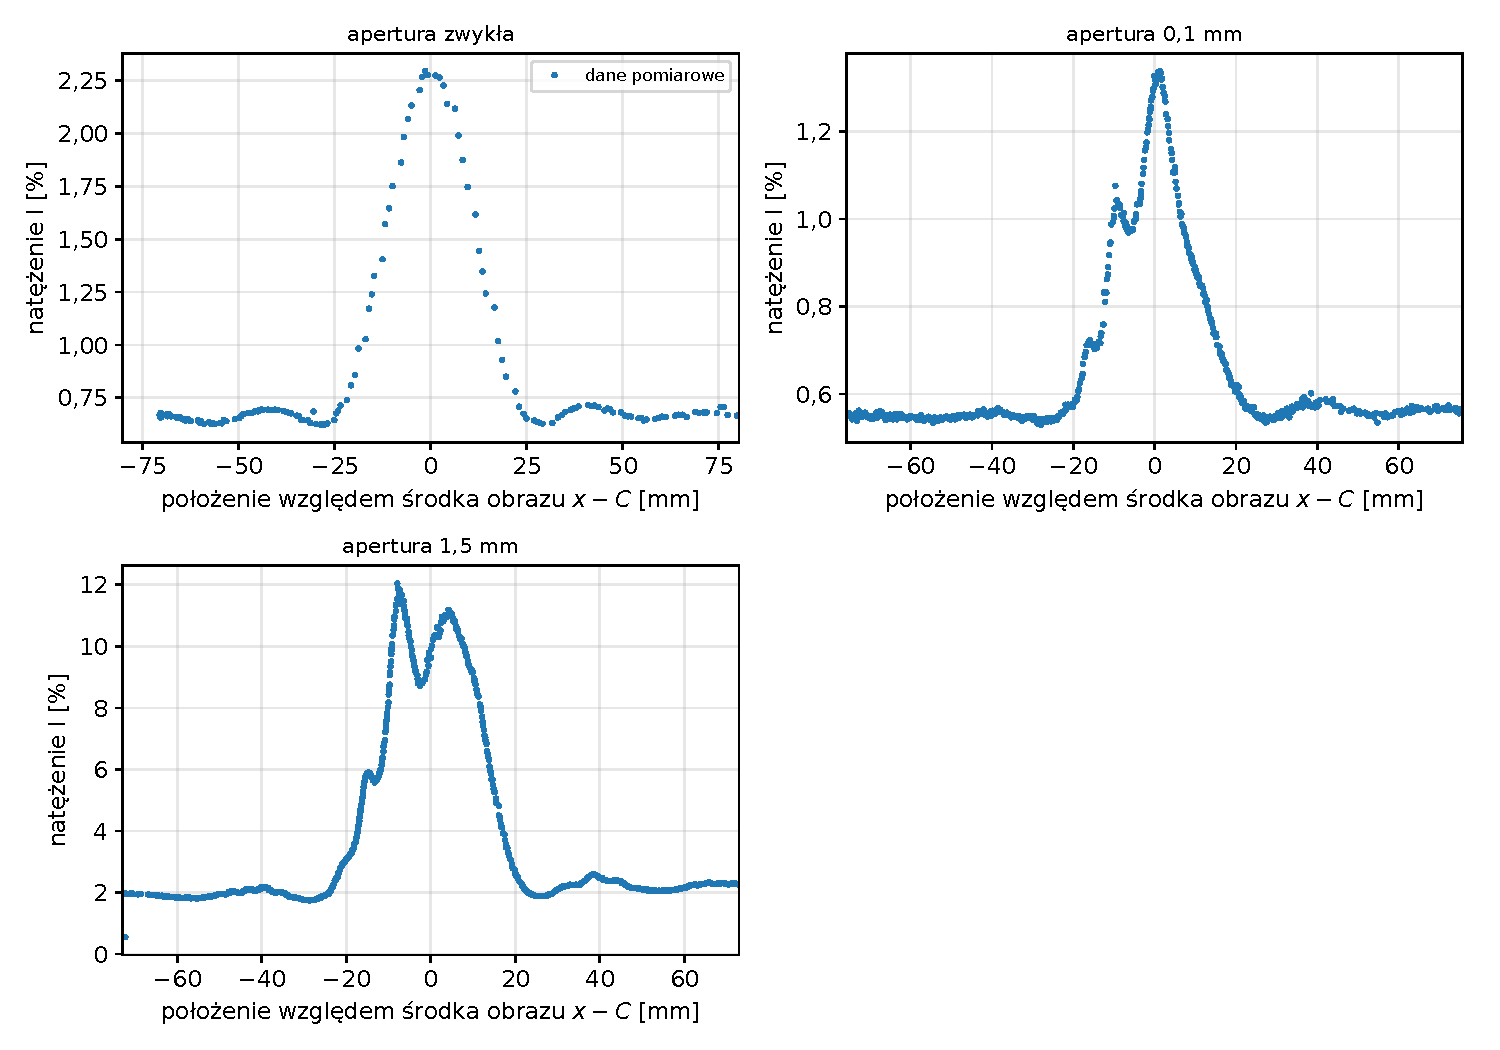
\includegraphics[width=0.9\textwidth]{aperture_raw.pdf}
    \caption{Rozkład natężenia za szczeliną $a_\text{nom} = 0{,}02$~mm, laser czerwony,
             $D = 900$~mm, dla apertury zwykłej, tj.\ używanej w pozostałych pomiarach
             (pierwszy przejazd z części Pojedyncza szczelina), i apertur $0{,}1$ oraz $1{,}5$~mm.}
    \label{fig:aperture_raw}
\end{figure}

% -------------------------------------------
\section{Opracowanie wyników}
% -------------------------------------------

\subsection{Kalibracja skali położenia}
\label{sec:calib}

Biblioteka \texttt{pasco} przelicza impulsy enkodera skanera na położenie stałą z opisu
czujnika: $\SI{0.01}{\meter}$ na 2000 impulsów. Pełny przesuw głowicy od ogranicznika do
ogranicznika wynosi według specyfikacji producenta $L_\text{spec} = 155$~mm~\cite{pasco}.
Wszystkie 58 przejazdów wykonano od ogranicznika do ogranicznika, a ich zapisana długość wynosi
$77{,}9$--$85{,}8$~mm (mediana $83{,}0$~mm), w obu sesjach i dla obu laserów. Przelicznik
biblioteki zaniża więc położenie mniej więcej dwukrotnie.

Rozrzut zapisanych długości nie oznacza różnej skali w różnych przejazdach. Gdyby przejazd
zapisany jako krótszy miał po prostu więcej zgubionych impulsów, obraz w nim byłby proporcjonalnie
węższy: $\mathrm{d}\ln B/\mathrm{d}\ln L = -1$. Regresja odchyleń $\ln B$ od $\ln L$ w obrębie
każdego układu (51 przejazdów, 17 układów) daje $\mathrm{d}\ln B/\mathrm{d}\ln L = 0{,}28 \pm 0{,}28$,
zgodne z zerem i niezgodne z $-1$ ($4{,}6\sigma$). Krótszy zapis wynika więc z obcięcia
przejazdu: program zapisywał go od ostatniego zawrotu skanera, który mógł wypaść kilka
milimetrów od ogranicznika (np.\ koniec przejazdu $a = 0{,}02$~mm nr~1 to $48{,}0$~mm, a początek
następnego przejazdu, wykonanego w przeciwną stronę, to $44{,}5$~mm). Skala jest natomiast
wspólna dla wszystkich przejazdów, a pełny przesuw najlepiej oddaje najdłuższy zapis,
$L_\text{rej} = 85{,}78$~mm:
\begin{equation}
    K_x = \frac{L_\text{spec}}{L_\text{rej}} = \frac{155}{85{,}78} = 1{,}807, \qquad
    \frac{u(K_x)}{K_x} = \sqrt{\left(\frac{u(L_\text{spec})}{L_\text{spec}}\right)^2
                       + \left(\frac{u(L_\text{rej})}{L_\text{rej}}\right)^2} = 0{,}9\,\%,
    \label{eq:Kx}
\end{equation}
gdzie $u(L_\text{spec}) = 1$~mm (ostatnia cyfra specyfikacji), a $u(L_\text{rej}) = 0{,}5$~mm
uwzględnia, że także najdłuższy zapis mógł być nieco obcięty (kolejne najdłuższe zapisy:
$85{,}4$; $84{,}9$; $84{,}8$~mm). Stąd
$K_x = 1{,}807 \pm 0{,}016$, i przez ten czynnik pomnożono wszystkie położenia $x$. Rzeczywisty
krok enkodera wynosi więc $1{,}807 \cdot \SI{5}{\micro\meter} = (9{,}04 \pm 0{,}08)~\si{\micro\meter}$,
zgodnie z rozdzielczością $0{,}01$~mm podaną w specyfikacji~\cite{pasco} (wartość zaokrąglona;
krok dokładnie $\SI{10}{\micro\meter}$ dawałby pełny przesuw $172$~mm zamiast 155~mm).
Przelicznik zapisany w bibliotece ($\SI{5}{\micro\meter}$ na impuls) jest więc po prostu
błędny dla tego skanera; ponieważ skala jest wspólna dla wszystkich przejazdów (niżej), nie jest
to losowa utrata impulsów. Kalibracja
jest niezależna od szczelin; jej poprawność sprawdzono, porównując wyniki z wymiarami
producenta (podsekcja~\ref{sec:scale}). Niepewność $u(K_x)/K_x$ wchodzi do części
systematycznej wyników tak samo jak $u_\lambda/\lambda$ i $u_D/D$.

\subsection{Metody i rachunek niepewności}

\paragraph{Dopasowanie krzywej.} Do każdego przejazdu dopasowano model~\eqref{eq:model_single}
(pojedyncza szczelina) lub~\eqref{eq:model_multi} (dwie i więcej szczelin, $N$ ustalone) funkcją
\texttt{scipy.optimize.curve\_fit}. Wartości startowe $B_a$ wzięto z szerokości połówkowej
maksimum centralnego ($\mathrm{FWHM} = 2{,}783/B_a$ dla funkcji $\mathrm{sinc}^2$), a $B_d$ ---
z odstępu sąsiednich prążków. Ponieważ funkcja $\mathrm{sinc}^2$ ma wiele minimów lokalnych,
dopasowanie startowano z kilku wartości $B_a$ i $C$ i wybierano to o najmniejszej sumie
kwadratów residuów. Dla wielu szczelin $C$ startowało także o jeden i dwa prążki obok
najwyższego punktu --- najwyższy punkt nie musi leżeć na prążku centralnym. Bez tego w dwóch
przejazdach ($N = 2$, przejazd 1, i $N = 3$, przejazd 2) model był przesunięty o jeden prążek.
Poprawka zmienia też szerokość połówkową maksimum centralnego (podsekcja Układy $N$ szczelin),
mierzoną wokół dopasowanego $C$. Dla $N = 3$, przejazd 2, przy przesuniętym $C$ mierzono
maksimum pierwszego rzędu: FWHM $= 1{,}12$~mm, a po poprawce $1{,}44$~mm. Średnia dla $N = 3$
wzrosła przez to z $1{,}30$ do $1{,}40$~mm. Niepewność pojedynczego odczytu
$I$ nie jest znana, dlatego dopasowanie jest nieważone (\texttt{absolute\_sigma=False}):
macierz kowariancji $V$ jest skalowana przez wariancję residuów, a $u(B) = \sqrt{V_{BB}}$.
Takie $u(B)$ zakłada nieskorelowane residua, a punkty są gęste względem struktury obrazu
i residua mają charakter systematyczny, więc $u(B)$ jest zaniżone. Rozrzut trzech
przejazdów przy tych samych ustawieniach jest ok.\ $1{,}8$ razy większy niż $u(B)$
z dopasowania (np.\ dla $a_\text{nom} = 0{,}02$~mm: $\sigma(s) = 0{,}22$~mm wobec
$u(s) = 0{,}12$~mm). Dlatego wynik końcowy opiera się na rozrzucie przejazdów, a nie na $u(B)$.

\paragraph{Regresja liniowa.} Położenie każdego minimum dyfrakcyjnego (lub maksimum
interferencyjnego) wyznaczono jako wierzchołek paraboli dopasowanej do punktów w oknie
$\pm0{,}3\,s$ wokół przewidywanego położenia, gdzie $s$ --- odstęp sąsiednich minimów (maksimów).
Dopasowanie krzywej służy tu tylko do przypisania rzędów $m$ i rozmieszczenia okien. Dla par
szczelin minima obwiedni nie są widoczne wprost, więc ich położenie to wierzchołek paraboli
dopasowanej do wysokości kolejnych prążków w otoczeniu zera obwiedni. Do punktów $(m, x_m)$
dopasowano prostą $x_m = x_0 + s\,m$ nieważoną metodą najmniejszych kwadratów
(\texttt{scipy.stats.linregress}); $u(s)$ to błąd standardowy nachylenia wyznaczony
z rozrzutu punktów.

\paragraph{Wynik końcowy.} Z każdego przejazdu $k$ obliczono $q_k = B_k\lambda D/\pi$
(dopasowanie) albo $q_k = \lambda D/s_k$ (regresja), gdzie $q$ oznacza $a$ lub $d$. Wynikiem
końcowym jest średnia $\bar q$ z $n = 3$ przejazdów. $\lambda$, $D$ i $K_x$ są wspólne dla wszystkich
przejazdów, więc ich niepewność nie maleje z liczbą powtórzeń i dodaje się ją osobno.
Z prawa propagacji niepewności dla $q = B\lambda D/\pi$:
\begin{equation}
    u(\bar q) = \sqrt{t^2\,\frac{\sigma^2(q)}{n}
              + \bar q^{\,2}\left[\left(\frac{u_\lambda}{\lambda}\right)^2
              + \left(\frac{u_D}{D}\right)^2 + \left(\frac{u(K_x)}{K_x}\right)^2\right]},
    \label{eq:u_final}
\end{equation}
gdzie $\sigma(q)$ --- odchylenie standardowe wyników z przejazdów, $t = 1{,}32$ ---
współczynnik Studenta dla $n = 3$ i poziomu ufności 68\,\%, a pierwszy składnik to
niepewność typu A, $u_A$. Część systematyczna wynosi
$\sqrt{0{,}8^2 + 1{,}6^2 + 0{,}9^2}\,\% \approx 2{,}0\,\%$ dla lasera czerwonego
i $\sqrt{1{,}0^2 + 1{,}6^2 + 0{,}9^2}\,\% \approx 2{,}1\,\%$ dla zielonego.
W większości wyników dominuje ona nad częścią statystyczną (np.\ dla $a_\text{nom} = 0{,}08$~mm,
laser czerwony: $u_A = 0{,}0005$~mm wobec $u_\text{sys} = 0{,}0015$~mm).

Obie metody korzystają z tych samych przejazdów i tych samych $\lambda$, $D$, więc ich wyniki
są skorelowane. Zgodność oceniono na różnicach z tych samych przejazdów,
$\Delta_k = q_{\text{fit},k} - q_{\text{reg},k}$, w których wspólne czynniki się znoszą:
\begin{equation}
    z = \frac{|\bar\Delta|}{u(\bar\Delta)}, \qquad u(\bar\Delta) = t\,\frac{\sigma(\Delta)}{\sqrt{n}}.
    \label{eq:z_methods}
\end{equation}
Przy $n = 3$ samo $\sigma(\Delta)$ jest wyznaczone niedokładnie, więc $z$ pokazuje raczej,
czy różnica metod jest powtarzalna, niż daje ścisły test; dlatego przy każdym $z$ podano
też względną różnicę metod.

\paragraph{Kierunek przejazdu.} Przejazdy wykonywano na przemian w obu kierunkach. Środek
obrazu $C$ z przejazdów w stronę rosnącego $x$ leży dalej niż z przejazdów w przeciwną
stronę, i to tym dalej, im szybszy przejazd: dla 34 par przejazdów tego samego układu
$C_\rightarrow - C_\leftarrow = (0{,}50 \pm 0{,}10)~\text{s}\cdot\bar v + (0{,}30 \pm 0{,}24)$~mm.
Odpowiada to opóźnieniu odczytu położenia względem odczytu natężenia o
$\tau = (250 \pm 50)$~ms: program pyta skaner o $x$ i $I$ dwoma osobnymi zapytaniami
Bluetooth. Przy stałej prędkości opóźnienie przesuwa cały obraz, ale nie zmienia odstępów.
Prędkość korbki nie jest jednak stała, a wahanie $\Delta v \approx 0{,}3$~mm/s przesuwa lokalnie
punkty o $\tau\,\Delta v \approx 0{,}08$~mm. Dlatego porównano parametry $B$ z przejazdów w obu
kierunkach: $B_\rightarrow/B_\leftarrow - 1 = (-0{,}7 \pm 0{,}9)\,\%$ dla $a$ (12 układów)
i $(+0{,}1 \pm 0{,}8)\,\%$ dla $d$ (11 układów). Kierunek przejazdu nie wpływa więc na $a$ ani $d$
w granicach niepewności, a nierównomierność ruchu korbki wchodzi do rozrzutu przejazdów
(ok.\ $3\,\%$ na pojedynczy przejazd), uwzględnionego w $u_A$.

\subsection{Pojedyncza szczelina}

Dopasowania przedstawiono na Rysunkach~\ref{fig:single_red} i~\ref{fig:single_green},
a regresje położeń minimów --- na Rysunku~\ref{fig:single_minima}. Model~\eqref{eq:model_single}
opisuje dane dobrze: RMS residuów wynosi $0{,}9$--$1{,}5\,\%$ wysokości maksimum. W zakresie
skanera mieściło się od 4 minimów ($a = 0{,}02$~mm, $m = \pm1, \pm2$) do 12 ($m = \pm1, \dots, \pm6$).
Wyniki zestawiono w Tabeli~\ref{tab:single}.

\begin{figure}[H]
    \centering
    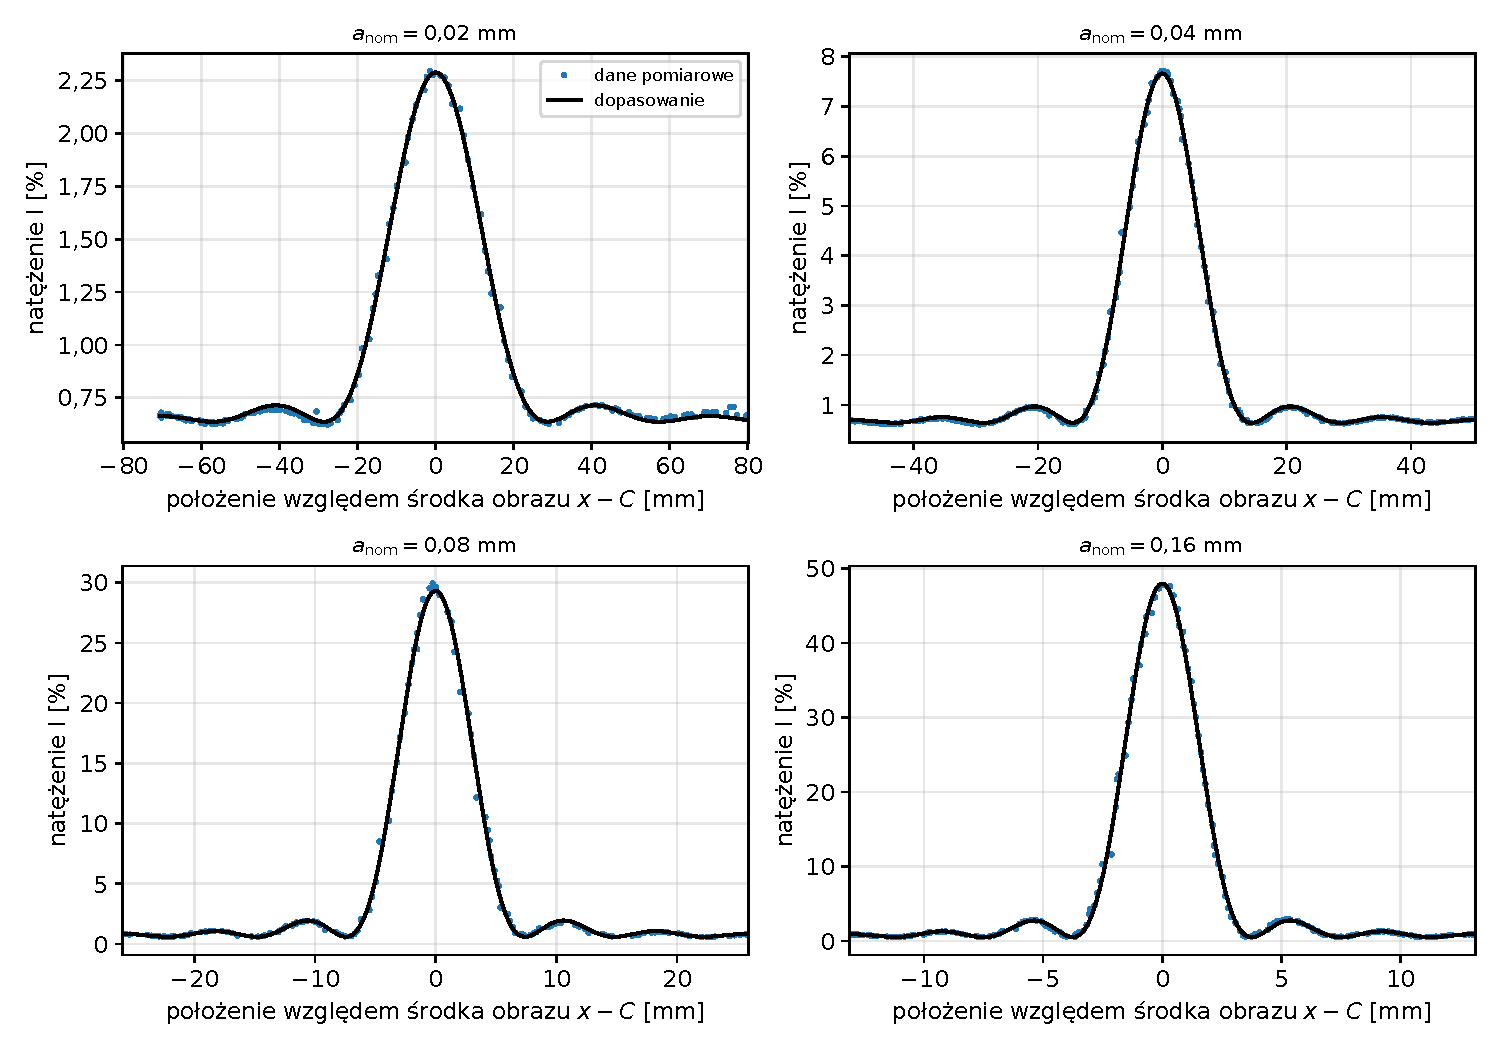
\includegraphics[width=0.9\textwidth]{single_slit_red.pdf}
    \caption{Rozkład natężenia za pojedynczą szczeliną (laser czerwony, pierwszy przejazd)
             z dopasowanym modelem~\eqref{eq:model_single} (linia ciągła).}
    \label{fig:single_red}
\end{figure}

\begin{figure}[H]
    \centering
    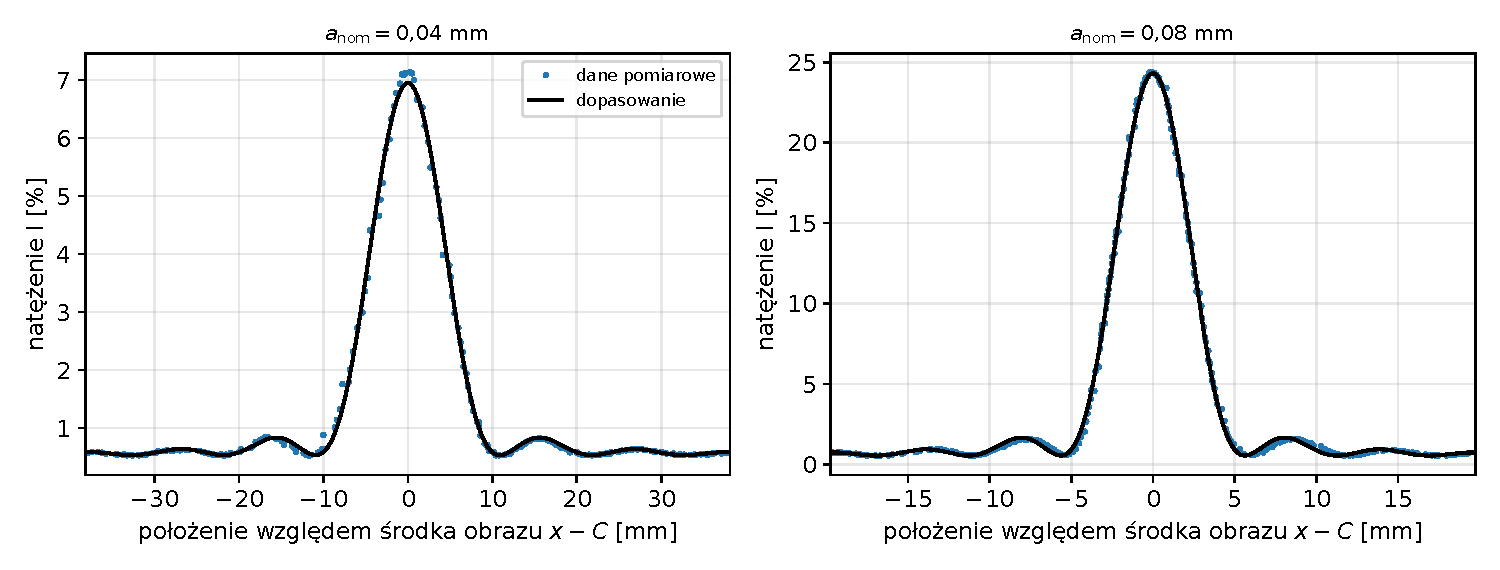
\includegraphics[width=0.9\textwidth]{single_slit_green.pdf}
    \caption{Rozkład natężenia za pojedynczą szczeliną (laser zielony, pierwszy przejazd)
             z dopasowanym modelem~\eqref{eq:model_single} (linia ciągła).}
    \label{fig:single_green}
\end{figure}

\begin{figure}[H]
    \centering
    \begin{subfigure}{0.48\textwidth}
        \centering
        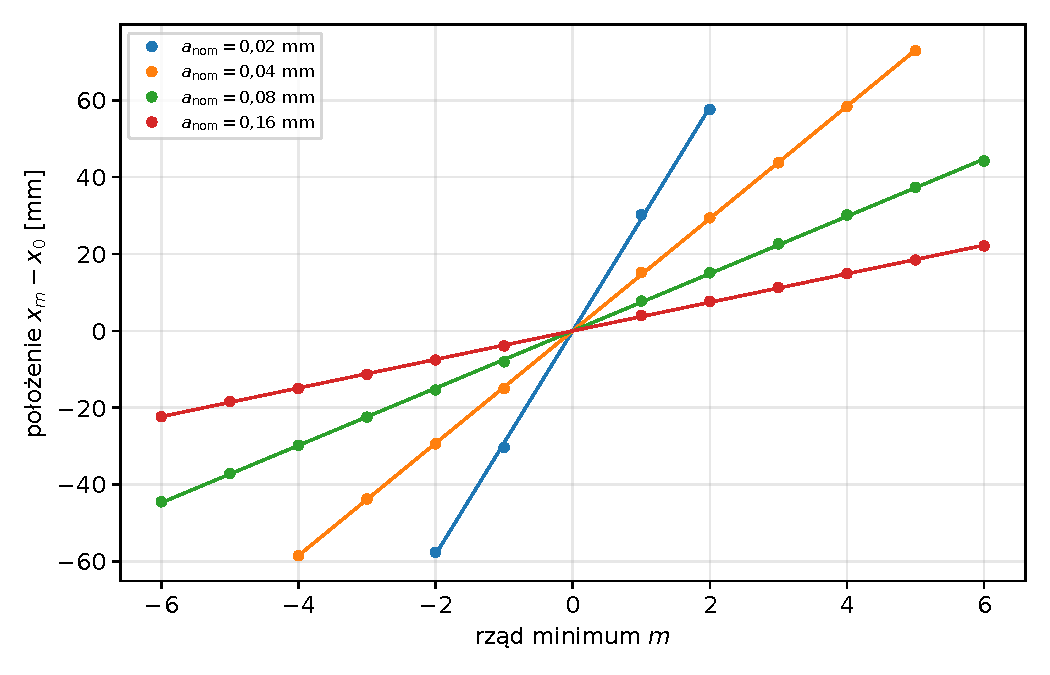
\includegraphics[width=\textwidth]{single_slit_minima_red.pdf}
        \caption{laser czerwony}
    \end{subfigure}
    \hfill
    \begin{subfigure}{0.48\textwidth}
        \centering
        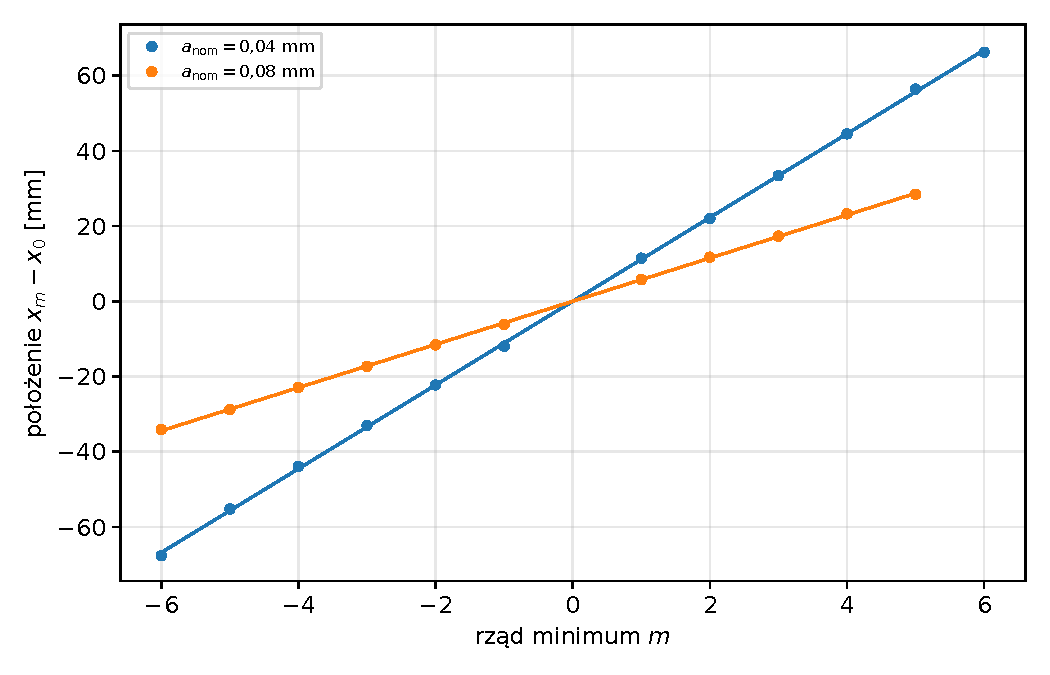
\includegraphics[width=\textwidth]{single_slit_minima_green.pdf}
        \caption{laser zielony}
    \end{subfigure}
    \caption{Położenia minimów dyfrakcyjnych względem wyrazu wolnego $x_0$ w funkcji rzędu $m$
             (pierwszy przejazd) z dopasowanymi prostymi; nachylenie $s = \lambda D/a$.}
    \label{fig:single_minima}
\end{figure}

\begin{table}[H]
    \centering
    \caption{Szerokość pojedynczej szczeliny z dopasowania ($a_\text{fit}$) i regresji
             ($a_\text{reg}$), stosunek do wartości producenta $k = a_\text{fit}/a_\text{nom}$,
             względna różnica metod $\delta = a_\text{fit}/a_\text{reg} - 1$ i jej
             powtarzalność $z$, wzór~\eqref{eq:z_methods}.}
    \label{tab:single}
    \begin{tabular}{l S[table-format=1.2] S[table-format=1.5]@{\,$\pm$\,}S[table-format=1.5]
                    S[table-format=1.5]@{\,$\pm$\,}S[table-format=1.5] S[table-format=1.2]
                    S[table-format=-1.1] S[table-format=1.1]}
        \toprule
        laser & {$a_\text{nom}$ [mm]} & \multicolumn{2}{c}{$a_\text{fit}$ [mm]}
              & \multicolumn{2}{c}{$a_\text{reg}$ [mm]} & {$k$} & {$\delta$ [\%]} & {$z$} \\
        \midrule
        czerwony & 0.02 & 0.02060 & 0.00042 & 0.02024 & 0.00043 & 1.03 & 1.8 & 3.6 \\
        czerwony & 0.04 & 0.0397 & 0.0011 & 0.03956 & 0.00093 & 0.99 & 0.2 & 0.3 \\
        czerwony & 0.08 & 0.0790 & 0.0016 & 0.0789 & 0.0016 & 0.99 & 0.2 & 0.5 \\
        czerwony & 0.16 & 0.1545 & 0.0036 & 0.1570 & 0.0035 & 0.97 & -1.6 & 4.4 \\
        zielony  & 0.04 & 0.04228 & 0.00089 & 0.04143 & 0.00086 & 1.06 & 2.1 & 3.4 \\
        zielony  & 0.08 & 0.0825 & 0.0018 & 0.0819 & 0.0018 & 1.03 & 0.7 & 0.8 \\
        \bottomrule
    \end{tabular}
\end{table}

Obie metody różnią się o najwyżej $2{,}1\,\%$, czyli mniej niż niepewność systematyczna
($2{,}0$--$2{,}1\,\%$). W trzech przypadkach różnica powtarza się we wszystkich przejazdach
($z = 3{,}4$--$4{,}4$), więc między metodami jest drobne systematyczne przesunięcie, o różnym
znaku dla różnych szczelin. Wyznaczone szerokości wynoszą $0{,}97$--$1{,}06$ wartości producenta
i są z nimi zgodne w granicach $3\sigma$ ($|a - a_\text{nom}|/u(a) = 0{,}3$--$1{,}6$ dla lasera
czerwonego). Największe odchylenie, $2{,}6\sigma$, ma szczelina $a_\text{nom} = 0{,}04$~mm dla lasera
zielonego; wszystkie wyniki zielone leżą nieco wyżej, co omówiono w podsekcji~\ref{sec:scale}.

Skalowanie obrazu z $1/a$ sprawdzono bez użycia wyznaczonego $a$: odstęp minimów $s = \pi/B_a$
pomnożony przez nominalną szerokość powinien być stały. Dla lasera czerwonego
$s\,a_\text{nom} = 0{,}568$; $0{,}590$; $0{,}592$; $0{,}606$~mm$^2$ dla $a_\text{nom} = 0{,}02$--$0{,}16$~mm
(niepewności $0{,}003$--$0{,}011$~mm$^2$), wobec $\lambda D = 0{,}585$~mm$^2$. Ośmiokrotna zmiana
$a_\text{nom}$ zmienia odstęp minimów ośmiokrotnie z dokładnością do $7\,\%$, ale reszta przekracza
niepewności. Uśrednianie natężenia po szerokości apertury $w$ poszerza obraz i daje ten sam znak:
dopasowanie $\mathrm{sinc}^2$ do rozkładu splecionego z prostokątem o $w = 0{,}5\,s$ zaniża $B$
o $6\,\%$. Dla $a_\text{nom} = 0{,}16$~mm ($s = 3{,}8$~mm) wymagałoby to $w \approx 1{,}9$~mm, więcej
niż największa apertura skanera ($1{,}5$~mm~\cite{pasco}), a taka apertura zmieniłaby wynik
dla $a_\text{nom} = 0{,}04$~mm tylko o ok.\ $0{,}3\,\%$, podczas gdy zmierzony skok między $0{,}02$
i $0{,}04$~mm wynosi $4\,\%$. Rozrzut odpowiada więc odchyleniom poszczególnych szczelin od
wymiarów nominalnych o kilka procent.

\subsection{Dwie szczeliny}

Dopasowania przedstawiono na Rysunkach~\ref{fig:double_red} i~\ref{fig:double_green},
a regresje położeń maksimów interferencyjnych --- na Rysunku~\ref{fig:double_maxima}. Wyniki
zestawiono w Tabeli~\ref{tab:double}.

\begin{figure}[H]
    \centering
    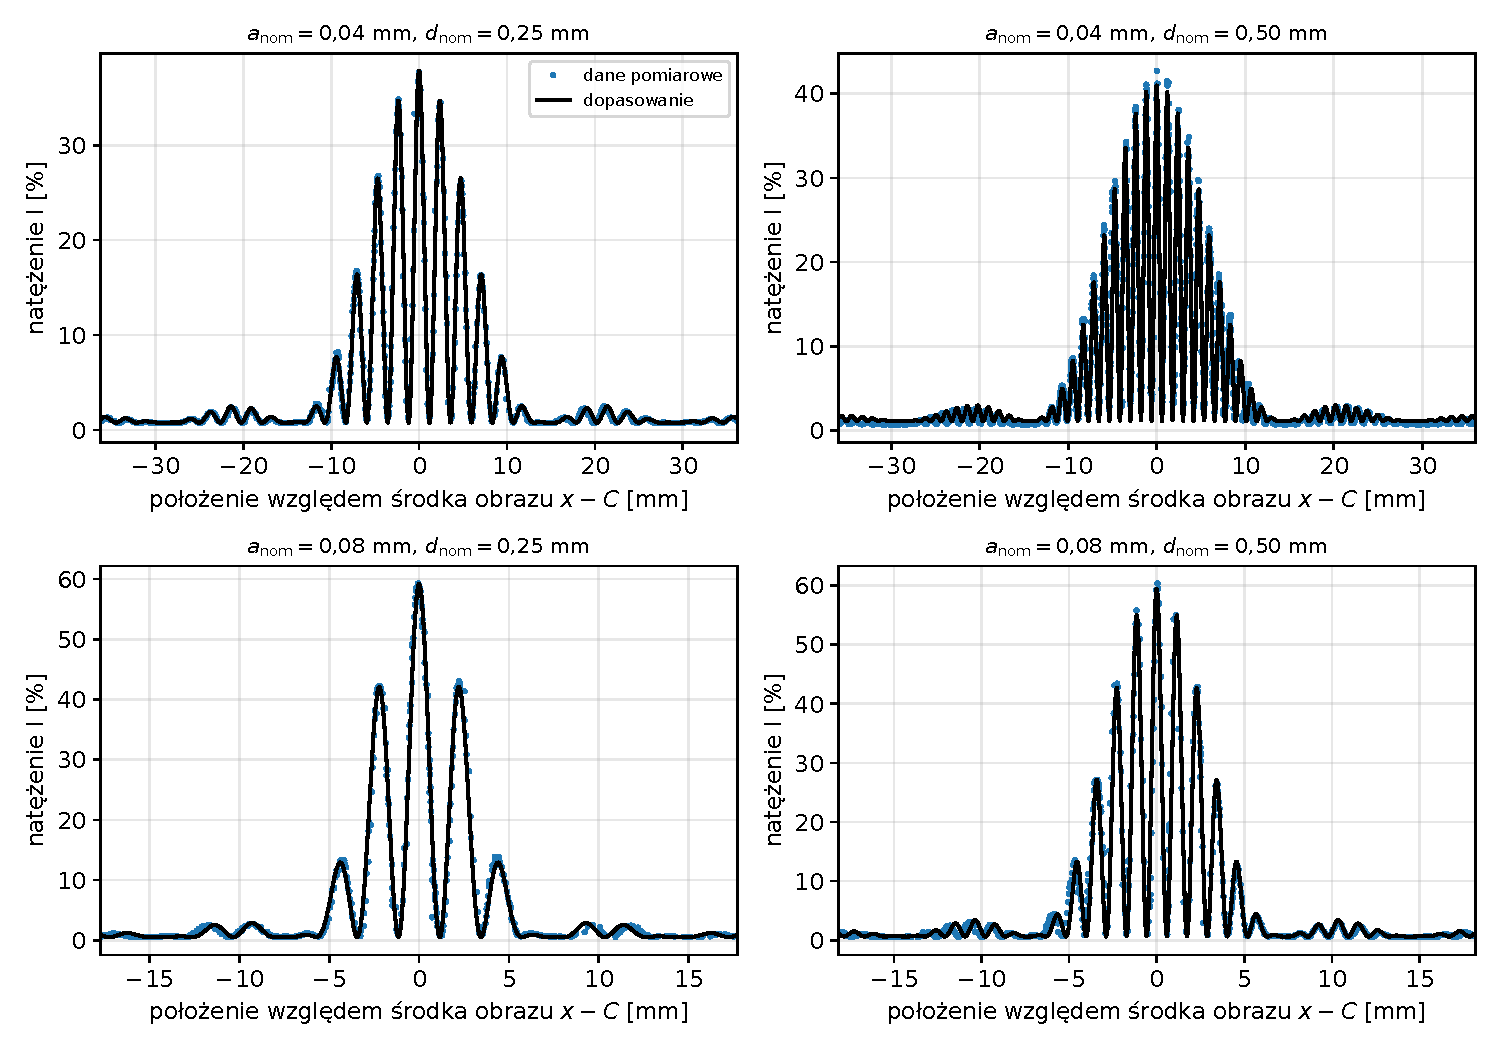
\includegraphics[width=0.9\textwidth]{double_slit_red.pdf}
    \caption{Rozkład natężenia za dwiema szczelinami (laser czerwony, pierwszy przejazd)
             z dopasowanym modelem~\eqref{eq:model_multi} dla $N = 2$ (linia ciągła).}
    \label{fig:double_red}
\end{figure}

\begin{figure}[H]
    \centering
    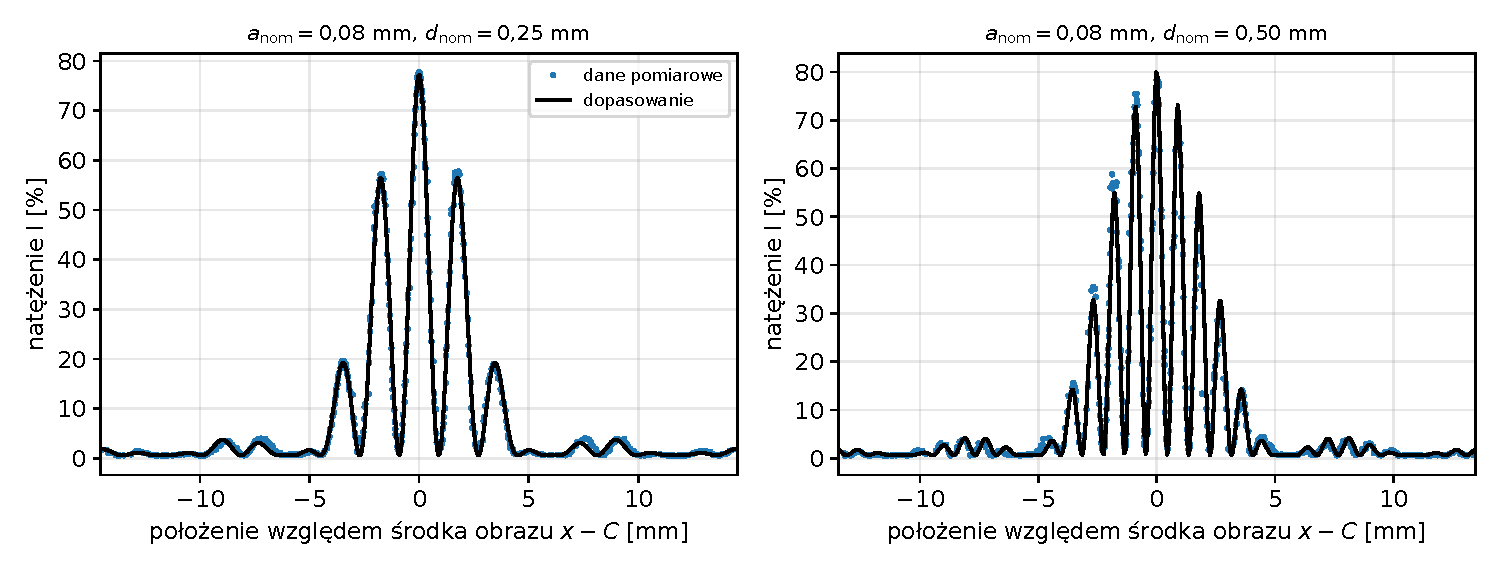
\includegraphics[width=0.9\textwidth]{double_slit_green.pdf}
    \caption{Rozkład natężenia za dwiema szczelinami (laser zielony, pierwszy przejazd)
             z dopasowanym modelem~\eqref{eq:model_multi} dla $N = 2$ (linia ciągła).}
    \label{fig:double_green}
\end{figure}

\begin{figure}[H]
    \centering
    \begin{subfigure}{0.48\textwidth}
        \centering
        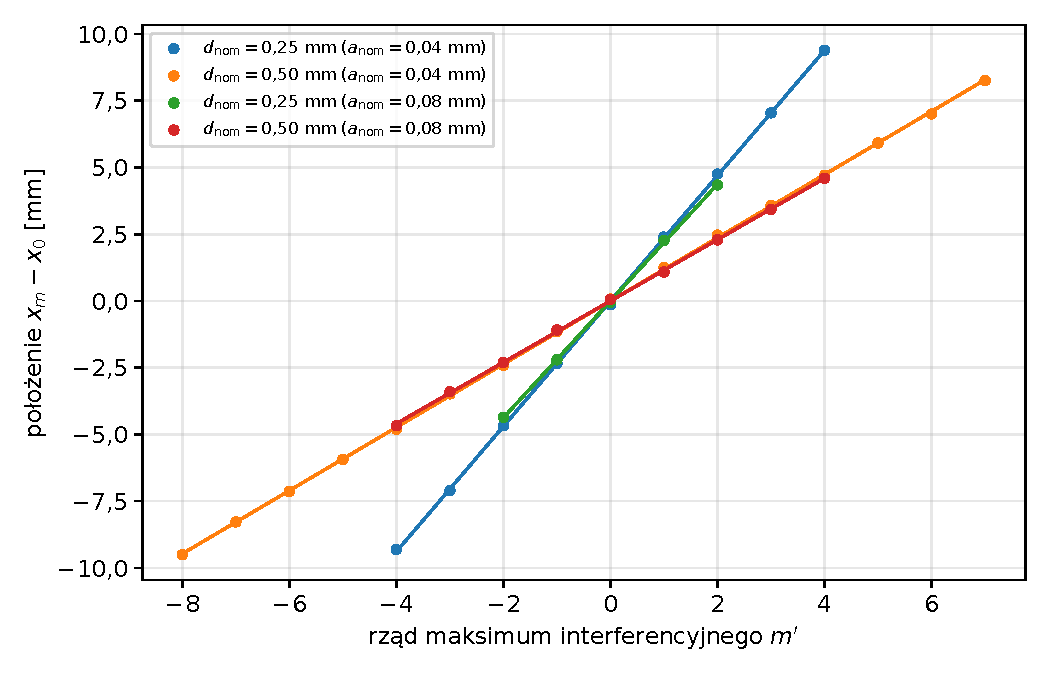
\includegraphics[width=\textwidth]{double_slit_maxima_red.pdf}
        \caption{laser czerwony}
    \end{subfigure}
    \hfill
    \begin{subfigure}{0.48\textwidth}
        \centering
        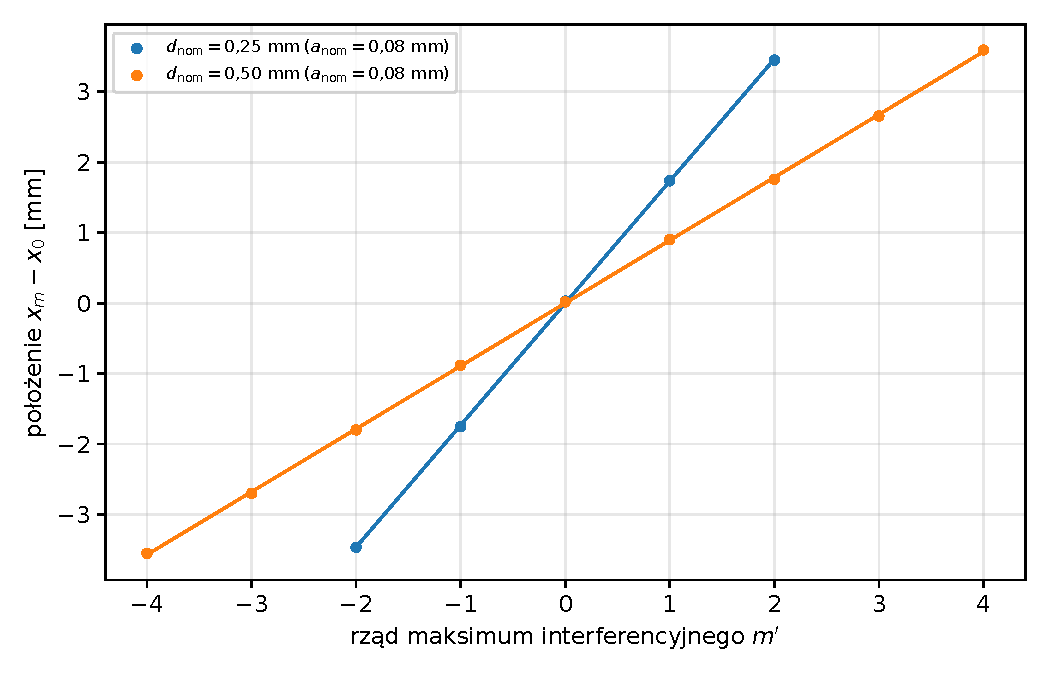
\includegraphics[width=\textwidth]{double_slit_maxima_green.pdf}
        \caption{laser zielony}
    \end{subfigure}
    \caption{Położenia maksimów interferencyjnych względem $x_0$ w funkcji rzędu $m'$
             (pierwszy przejazd) z dopasowanymi prostymi; nachylenie $s = \lambda D/d$.}
    \label{fig:double_maxima}
\end{figure}

\begin{table}[H]
    \centering
    \caption{Szerokość szczelin $a$ i odległość między szczelinami $d$ dla par szczelin
             z dopasowania (fit) i regresji (reg) oraz powtarzalność różnicy metod $z_a$, $z_d$,
             wzór~\eqref{eq:z_methods}.}
    \label{tab:double}
    \footnotesize
    \begin{tabular}{l S[table-format=1.2] S[table-format=1.2]
                    S[table-format=1.4]@{\,$\pm$\,}S[table-format=1.4]
                    S[table-format=1.4]@{\,$\pm$\,}S[table-format=1.4]
                    S[table-format=1.4]@{\,$\pm$\,}S[table-format=1.4]
                    S[table-format=1.4]@{\,$\pm$\,}S[table-format=1.4]
                    S[table-format=1.1] S[table-format=1.1]}
        \toprule
        laser & {$a_\text{nom}$} & {$d_\text{nom}$} & \multicolumn{2}{c}{$a_\text{fit}$ [mm]}
              & \multicolumn{2}{c}{$a_\text{reg}$ [mm]} & \multicolumn{2}{c}{$d_\text{fit}$ [mm]}
              & \multicolumn{2}{c}{$d_\text{reg}$ [mm]} & {$z_a$} & {$z_d$} \\
        \midrule
        czerwony & 0.04 & 0.25 & 0.0409 & 0.0014 & 0.03887 & 0.00085 & 0.2454 & 0.0049 & 0.2502 & 0.0061 & 2.2 & 1.9 \\
        czerwony & 0.04 & 0.50 & 0.0422 & 0.0016 & 0.03719 & 0.00080 & 0.504 & 0.012 & 0.502 & 0.011 & 4.5 & 0.4 \\
        czerwony & 0.08 & 0.25 & 0.0797 & 0.0030 & 0.0777 & 0.0017 & 0.241 & 0.011 & 0.2573 & 0.0083 & 0.7 & 3.9 \\
        czerwony & 0.08 & 0.50 & 0.0789 & 0.0021 & 0.0764 & 0.0017 & 0.499 & 0.015 & 0.499 & 0.016 & 4.0 & 0.2 \\
        zielony  & 0.08 & 0.25 & 0.0810 & 0.0022 & 0.0787 & 0.0017 & 0.2558 & 0.0054 & 0.2689 & 0.0058 & 2.2 & 4.3 \\
        zielony  & 0.08 & 0.50 & 0.0843 & 0.0022 & 0.0803 & 0.0019 & 0.505 & 0.014 & 0.510 & 0.017 & 4.1 & 1.5 \\
        \bottomrule
    \end{tabular}
\end{table}

Odległości $d$ z obu metod różnią się o najwyżej $2\,\%$ poza parą $a = 0{,}08$~mm,
$d = 0{,}25$~mm, gdzie regresja daje $d$ większe o $5\,\%$ (laser zielony, $z_d = 4{,}3$)
i $7\,\%$ (czerwony, $z_d = 3{,}9$). Dla $d/a = 3{,}1$ w maksimum centralnym obwiedni mieści
się tylko 5 prążków, a prążki $m' = \pm2$ leżą na stromym zboczu obwiedni $\mathrm{sinc}^2$.
Iloczyn $\cos^2 \cdot \mathrm{sinc}^2$ przesuwa wtedy maksima w stronę środka obrazu, więc
odstęp wierzchołków jest mniejszy niż $\lambda D/d$, a regresja zawyża $d$. Dopasowanie
uwzględnia obwiednię jawnie i nie ma tego błędu.

Szerokości $a$ z regresji minimów obwiedni są we wszystkich sześciu przypadkach mniejsze niż
z dopasowania (o $2{,}6$--$13{,}5\,\%$, $z_a = 0{,}7$--$4{,}5$). Położenie zera obwiedni
wyznaczano z wysokości zaledwie 3--4 prążków, więc za wynik bardziej wiarygodny przyjęto
dopasowanie. Szerokości z dopasowania zgadzają się z wynikami dla pojedynczych szczelin o tym
samym $a_\text{nom}$ (laser czerwony, $a_\text{nom} = 0{,}08$~mm: $0{,}0797 \pm 0{,}0030$
i $0{,}0789 \pm 0{,}0021$~mm wobec $0{,}0790 \pm 0{,}0016$~mm). Odległości $d$ z dopasowania są
zgodne z wartościami producenta ($|d - d_\text{nom}|/u(d) \le 1{,}1$), a szerokości $a$ --- w granicach
$2\sigma$.

Warunek pola dalekiego jest tu spełniony słabiej niż dla pojedynczych szczelin: dla pary
$a = 0{,}08$~mm, $d = 0{,}50$~mm rozmiar całej struktury $L = d + a = 0{,}58$~mm daje
$L^2/\lambda \approx 520$~mm, czyli liczbę Fresnela $F = L^2/(\lambda D) \approx 0{,}6$. Dla dwóch
symetrycznych szczelin człony kwadratowe fazy $(y \mp d/2)^2/(2D)$ różnią się jednak tylko
o $yd/D$, czyli o człon z przybliżenia Fraunhofera, więc położenia prążków nie zależą od $F$.
Każda szczelina z osobna ($a^2/\lambda \le 10$~mm) jest w polu dalekim.

\subsection{Układy $N$ szczelin}

Dopasowania modelu~\eqref{eq:model_multi} przedstawiono na Rysunku~\ref{fig:multi},
a wyniki --- w Tabelach~\ref{tab:multi} i~\ref{tab:multi_shape}. Dla każdego przejazdu
zmierzono też szerokość połówkową (FWHM) centralnego maksimum głównego i policzono maksima
poboczne między maksimum centralnym a pierwszymi maksimami głównymi (w danych uśrednionych
co $0{,}05$~mm, próg $0{,}5\,\%$ wysokości maksimum).

\begin{figure}[H]
    \centering
    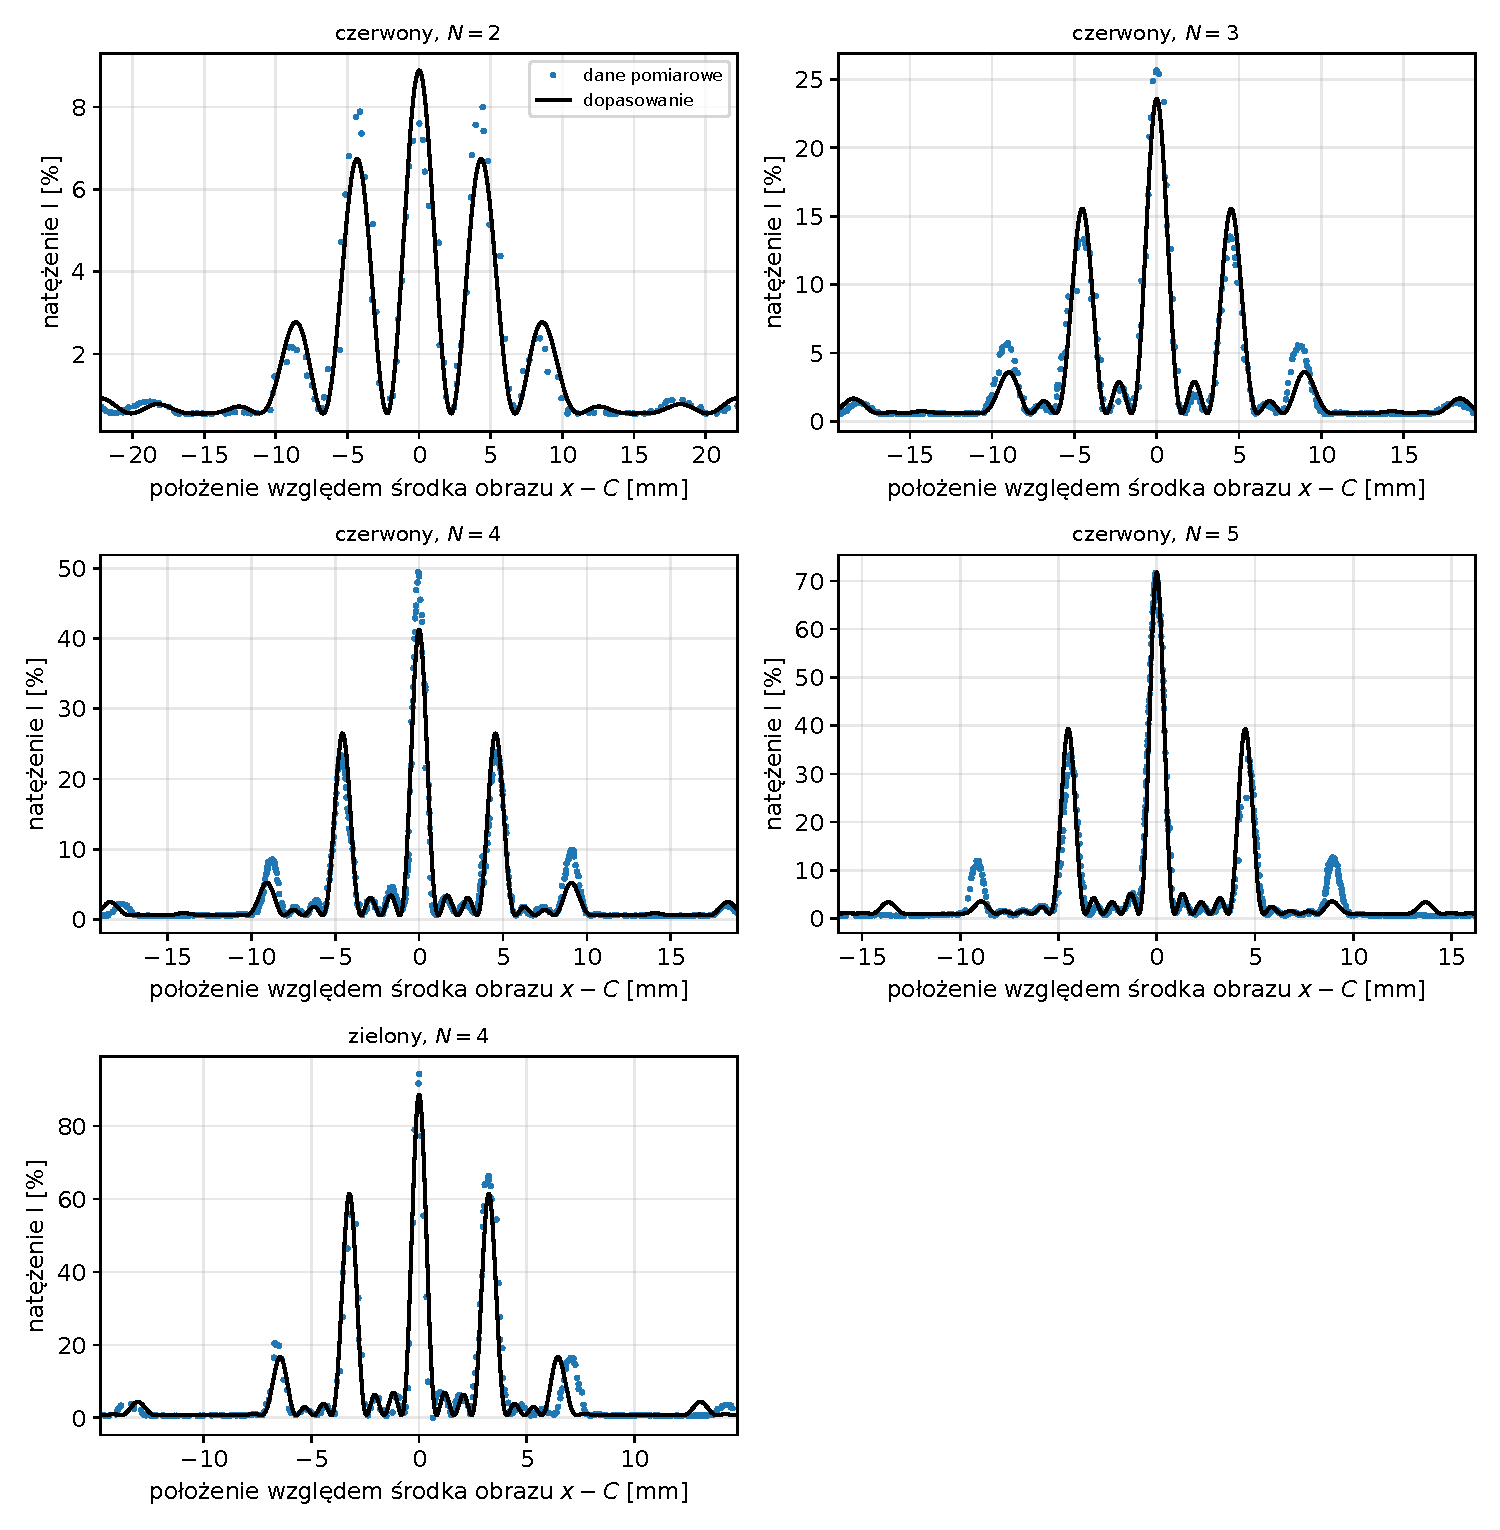
\includegraphics[width=0.9\textwidth]{multi_slit.pdf}
    \caption{Rozkład natężenia dla układów $N$ szczelin ($a_\text{nom} = 0{,}04$~mm,
             $d_\text{nom} = 0{,}125$~mm, pierwszy przejazd) z dopasowanym
             modelem~\eqref{eq:model_multi} (linia ciągła).}
    \label{fig:multi}
\end{figure}

\begin{table}[H]
    \centering
    \caption{Układy $N$ szczelin: $a$ i $d$ z dopasowania, $d$ z regresji położeń maksimów
             głównych, względna różnica metod $\delta_d = d_\text{fit}/d_\text{reg} - 1$
             i jej powtarzalność $z_d$, wzór~\eqref{eq:z_methods}.}
    \label{tab:multi}
    \begin{tabular}{l S[table-format=1.0]
                    S[table-format=1.4]@{\,$\pm$\,}S[table-format=1.4]
                    S[table-format=1.4]@{\,$\pm$\,}S[table-format=1.4]
                    S[table-format=1.4]@{\,$\pm$\,}S[table-format=1.4]
                    S[table-format=-1.1] S[table-format=1.1]}
        \toprule
        laser & {$N$} & \multicolumn{2}{c}{$a_\text{fit}$ [mm]} & \multicolumn{2}{c}{$d_\text{fit}$ [mm]}
              & \multicolumn{2}{c}{$d_\text{reg}$ [mm]} & {$\delta_d$ [\%]} & {$z_d$} \\
        \midrule
        czerwony & 2 & 0.0418 & 0.0019 & 0.1298 & 0.0031 & 0.1353 & 0.0038 & -4.1 & 4.3 \\
        czerwony & 3 & 0.0438 & 0.0025 & 0.1288 & 0.0028 & 0.1308 & 0.0026 & -1.6 & 1.7 \\
        czerwony & 4 & 0.0443 & 0.0022 & 0.1276 & 0.0025 & 0.1290 & 0.0026 & -1.1 & 1.2 \\
        czerwony & 5 & 0.0512 & 0.0023 & 0.1300 & 0.0027 & 0.1311 & 0.0027 & -0.8 & 5.3 \\
        zielony  & 4 & 0.0447 & 0.0022 & 0.1324 & 0.0071 & 0.1321 & 0.0046 & 0.2 & 0.1 \\
        \bottomrule
    \end{tabular}
\end{table}

\begin{table}[H]
    \centering
    \caption{Kształt obrazu układów $N$ szczelin (średnie z trzech przejazdów): szerokość
             połówkowa centralnego maksimum głównego, wartość teoretyczna
             $\mathrm{FWHM}_\text{teor}$ ze wzoru~\eqref{eq:n_slits} dla zmierzonego $B_d$,
             zgodność $z = |\mathrm{FWHM} - \mathrm{FWHM}_\text{teor}|/u(\mathrm{FWHM})$,
             największe natężenie $I_\text{max}$ i liczba maksimów pobocznych po lewej / prawej
             stronie maksimum centralnego (mediana).}
    \label{tab:multi_shape}
    \begin{tabular}{l S[table-format=1.0]
                    S[table-format=1.3]@{\,$\pm$\,}S[table-format=1.3]
                    S[table-format=1.3] S[table-format=1.1]
                    S[table-format=2.1]@{\,$\pm$\,}S[table-format=1.1] c}
        \toprule
        laser & {$N$} & \multicolumn{2}{c}{FWHM [mm]} & {$\mathrm{FWHM}_\text{teor}$ [mm]} & {$z$}
              & \multicolumn{2}{c}{$I_\text{max}$ [\%]} & poboczne \\
        \midrule
        czerwony & 2 & 2.467 & 0.096 & 2.253 & 2.2 & 10.1 & 1.5 & 0/0 \\
        czerwony & 3 & 1.403 & 0.089 & 1.411 & 0.1 & 23.7 & 2.2 & 1/1 \\
        czerwony & 4 & 0.98  & 0.10  & 1.044 & 0.6 & 45.5 & 4.0 & 2/2 \\
        czerwony & 5 & 0.870 & 0.062 & 0.811 & 1.0 & 70.8 & 0.9 & 3/3 \\
        zielony  & 4 & 0.870 & 0.049 & 0.797 & 1.5 & 93.1 & 1.4 & 2/2 \\
        \bottomrule
    \end{tabular}
\end{table}

Wyniki porównano z przewidywaniami wzoru~\eqref{eq:full}:
\begin{itemize}
    \item Odległość $d$ nie zależy od $N$: dla lasera czerwonego $d_\text{fit} = 0{,}128$--$0{,}130$~mm
          dla wszystkich $N$ (wobec $d_\text{nom} = 0{,}125$~mm, $|d - d_\text{nom}|/u(d) \le 1{,}9$), a metody różnią się o najwyżej $4\,\%$ (największa różnica dla $N = 2$,
          gdzie maksima główne są najszersze). Położenia maksimów głównych są więc niezależne
          od liczby szczelin, jak wynika ze wzoru~\eqref{eq:young_max}.
    \item Między maksimum centralnym a pierwszym maksimum głównym z każdej strony występuje
          $N - 2$ maksimów pobocznych (mediana z trzech przejazdów).
    \item Maksimum główne zwęża się ze wzrostem $N$: FWHM maleje od $2{,}47$~mm ($N = 2$)
          do $0{,}87$~mm ($N = 5$) i zgadza się z wartością teoretyczną w granicach niepewności
          ($z \le 2{,}2$). Odchylenia mają oba znaki ($-6$ do $+10\,\%$), więc nie dominuje
          poszerzenie przez aperturę czujnika, które dawałoby zawsze FWHM większe od teorii.
    \item Natężenie maksimum głównego rośnie z $N$. Regresja ważona $\ln I_\text{max} = \ln c + p\ln N$
          (wagi z rozrzutu przejazdów) daje $p = 2{,}12 \pm 0{,}12$, zgodne z $p = 2$
          ($|p - 2|/u(p) = 1{,}0$): amplitudy fal z $N$ szczelin dodają się w fazie. Porównanie
          wymaga stałej czułości i apertury w całej serii. Nie zanotowano tego wprost, ale
          zmiana apertury zmienia natężenie kilkukrotnie (część Zmiana apertury czujnika),
          a $I_\text{max}/N^2 = 2{,}5$; $2{,}6$; $2{,}8$; $2{,}8\,\%$ zmienia się płynnie, bez skoku.
          Nie wyklucza to zmiany czułości na poziomie samego trendu ($2{,}5 \to 2{,}8$, ok.\ $12\,\%$),
          która przesunęłaby $p$ o ok.\ $0{,}1$, czyli w granicach $u(p)$.
\end{itemize}
Szerokość $a$ z dopasowania rośnie z $N$ od $0{,}042$ do $0{,}051$~mm, a dla $N = 5$ model
nie odtwarza wysokości maksimów głównych drugiego rzędu (dane ok.\ $12\,\%$, model ok.\ $3\,\%$
przy maksimum centralnym ok.\ $71\,\%$, Rysunek~\ref{fig:multi}). Obwiednia zmienia się na odległości
$\lambda D/a \approx 15$~mm i działa tylko na kilka wąskich maksimów głównych, więc $a$ jest tu
wyznaczane z wysokości kilku prążków i obciążone każdą niejednorodnością oświetlenia
szczelin. Dlatego $a$ z układów $N$ szczelin nie jest wynikiem i nie weszło do średniej
w podsekcji~\ref{sec:scale}. Dla $N = 5$ struktura ma szerokość $L = 4d + a = 0{,}54$~mm
($F \approx 0{,}5$), a człon kwadratowy fazy skrajnych szczelin, $\pi(2d)^2/(\lambda D) \approx
0{,}34$~rad, nie znosi się jak dla dwóch szczelin. Zmienia on głębokość minimów i wysokość
maksimów pobocznych, ale nie położenia maksimów głównych.

Zgodnie z Dodatkiem~B porównano obwiednię rozkładów dla dwóch szczelin ze znormalizowanym
rozkładem pojedynczych szczelin (Rysunek~\ref{fig:envelope}). Wierzchołki prążków pary
o $a_\text{nom} = 0{,}04$~mm układają się na rozkładzie pojedynczej szczeliny $0{,}04$~mm,
a pary o $a_\text{nom} = 0{,}08$~mm --- na rozkładzie szczeliny $0{,}08$~mm: obraz
interferencyjny jest modulowany obrazem dyfrakcyjnym pojedynczej szczeliny, jak we
wzorze~\eqref{eq:full}.

\begin{figure}[H]
    \centering
    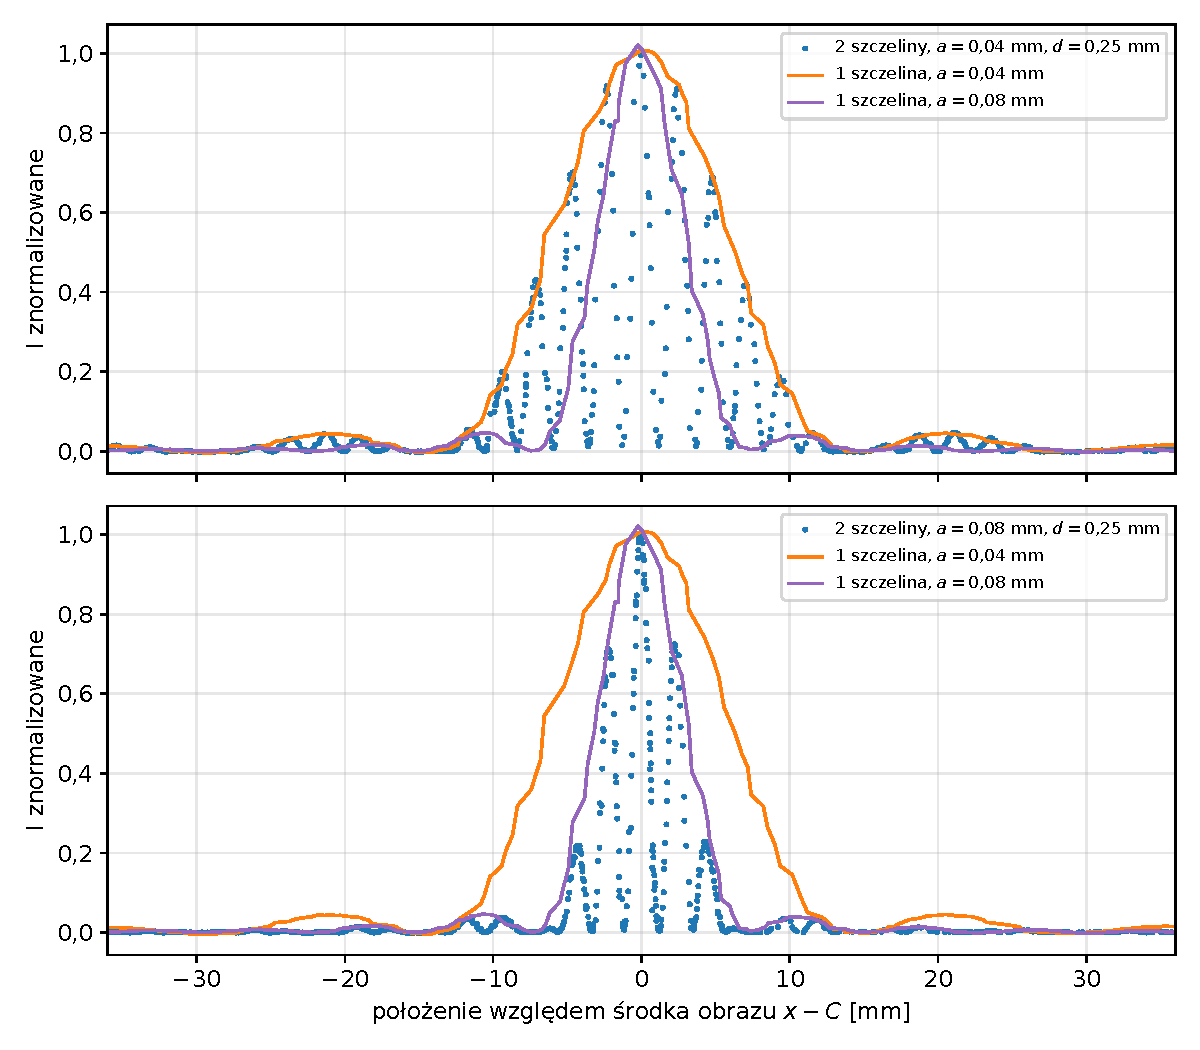
\includegraphics[width=0.75\textwidth]{envelope_comparison.pdf}
    \caption{Znormalizowany rozkład natężenia dla par szczelin o $d_\text{nom} = 0{,}25$~mm
             (punkty) i pojedynczych szczelin $a_\text{nom} = 0{,}04$ i $0{,}08$~mm (linie),
             laser czerwony, po odjęciu tła $b$ i podzieleniu przez $A$ z dopasowania.}
    \label{fig:envelope}
\end{figure}

\subsection{Zmiana odległości szczelina--detektor}

Dopasowania dla czterech odległości przedstawiono na Rysunku~\ref{fig:distance}, a odstępy
minimów $s$ --- w Tabeli~\ref{tab:distance}. Kształt maksimum centralnego przy $D = 400$, $500$
i $1000$~mm jest zniekształcony (RMS residuów $4$--$6\,\%$ wysokości maksimum, wobec
$1{,}3\,\%$ dla $D = 900$~mm), ale jego szerokość model nadal odtwarza.

\begin{figure}[H]
    \centering
    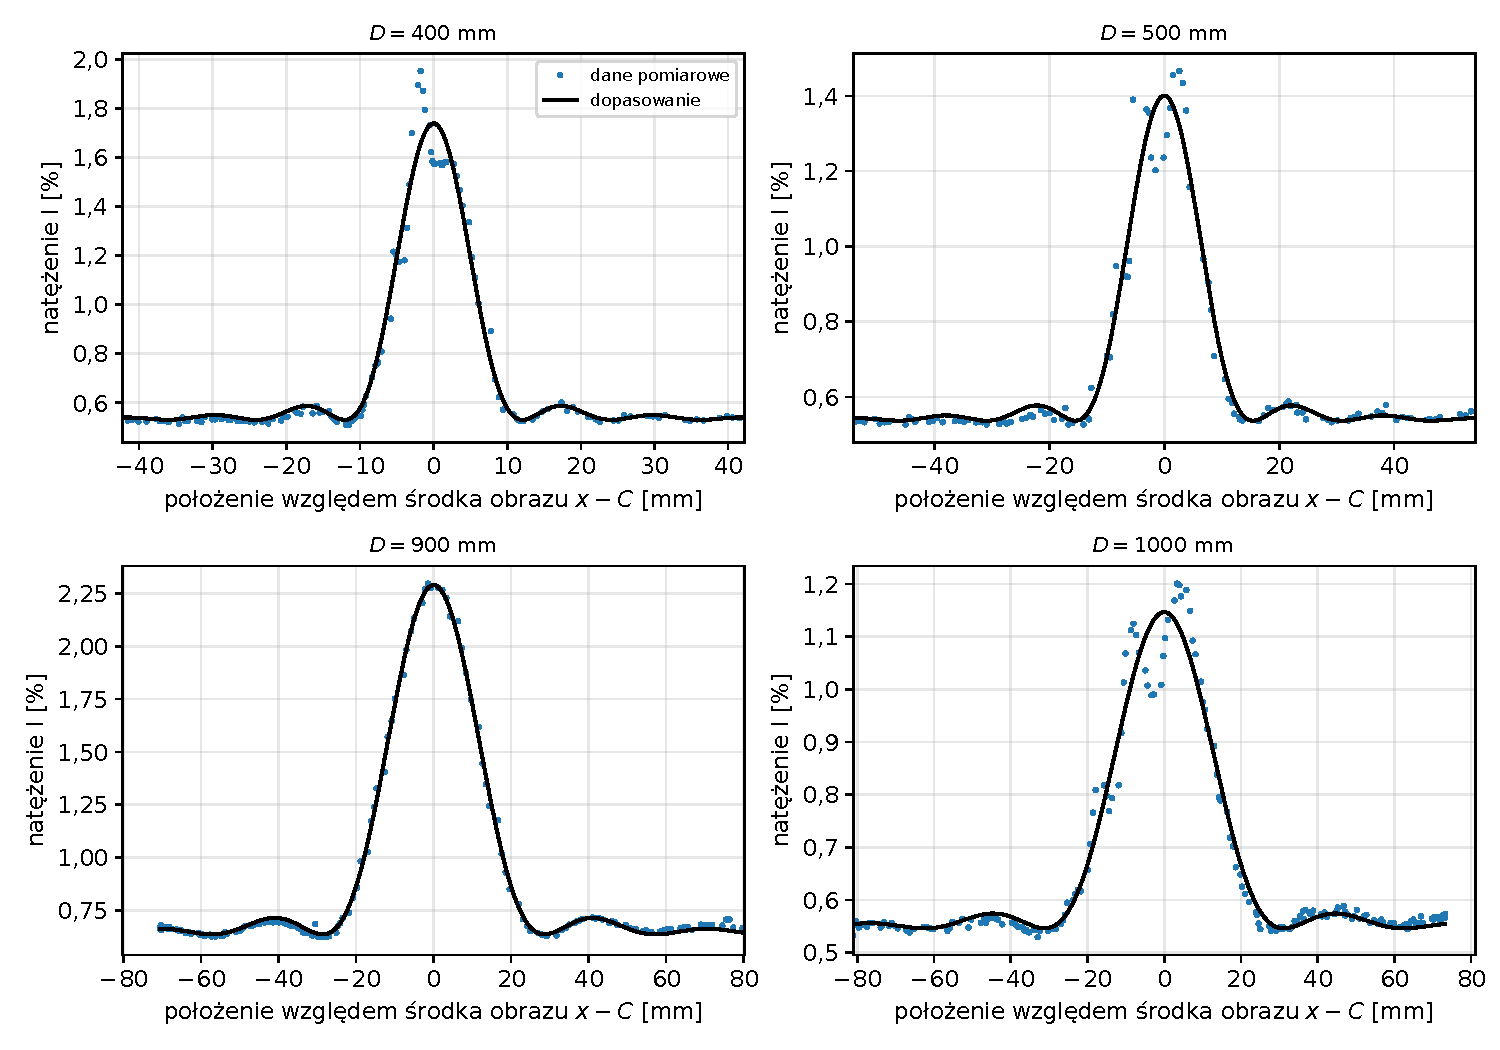
\includegraphics[width=0.9\textwidth]{distance.pdf}
    \caption{Rozkład natężenia za szczeliną $a_\text{nom} = 0{,}02$~mm (laser czerwony) dla
             różnych odległości $D$ z dopasowanym modelem~\eqref{eq:model_single} (linia ciągła).}
    \label{fig:distance}
\end{figure}

\begin{table}[H]
    \centering
    \caption{Odstęp minimów $s$ z dopasowania ($s = \pi/B_a$) i z regresji położeń minimów
             w funkcji odległości $D$; $n_\text{min}$ --- liczba minimów w regresji, $a$ ---
             szerokość szczeliny $\lambda D/s$ z każdego przejazdu. Niepewności $u(s)$ z jednego
             przejazdu są zaniżone ok.\ $1{,}8$ razy (podsekcja Metody i rachunek niepewności).}
    \label{tab:distance}
    \begin{tabular}{S[table-format=4.0] S[table-format=2.3]@{\,$\pm$\,}S[table-format=1.3]
                    S[table-format=2.3]@{\,$\pm$\,}S[table-format=1.3] S[table-format=1.0]
                    S[table-format=1.4] S[table-format=1.4]}
        \toprule
        {$D$ [mm]} & \multicolumn{2}{c}{$s_\text{fit}$ [mm]} & \multicolumn{2}{c}{$s_\text{reg}$ [mm]}
                   & {$n_\text{min}$} & {$a_\text{fit}$ [mm]} & {$a_\text{reg}$ [mm]} \\
        \midrule
        400  & 12.07 & 0.16 & 11.903 & 0.065 & 9 & 0.0215 & 0.0218 \\
        500  & 15.46 & 0.28 & 15.46 & 0.17 & 7 & 0.0210 & 0.0210 \\
        900  & 28.64 & 0.11 & 29.08 & 0.41 & 4 & 0.0204 & 0.0201 \\
        900  & 28.21 & 0.12 & 28.56 & 0.31 & 4 & 0.0207 & 0.0205 \\
        900  & 28.34 & 0.14 & 29.06 & 0.32 & 4 & 0.0206 & 0.0201 \\
        1000 & 31.21 & 0.46 & 31.24 & 0.23 & 4 & 0.0208 & 0.0208 \\
        \bottomrule
    \end{tabular}
\end{table}

Zgodnie ze wzorem~\eqref{eq:minima} odstęp minimów rośnie liniowo z $D$:
\begin{equation}
    s = \frac{\lambda}{a}\,D + c,
    \label{eq:s_vs_D}
\end{equation}
gdzie $c$ --- wyraz wolny, różny od zera, gdyby $D$ było obarczone stałym przesunięciem
$\Delta D = c/(\lambda/a)$ (np.\ płaszczyzna czujnika w innym miejscu niż odczyt na ławie).
Nieważona regresja liniowa (Rysunek~\ref{fig:distance_scaling}) daje:
\begin{itemize}
    \item z dopasowania: $\lambda/a = (0{,}03221 \pm 0{,}00043)$, $c = (-0{,}71 \pm 0{,}35)$~mm,
          $R^2 = 0{,}9993$, skąd $a = (0{,}0202 \pm 0{,}0004)$~mm;
    \item z regresji minimów: $\lambda/a = (0{,}03308 \pm 0{,}00086)$, $c = (-1{,}14 \pm 0{,}69)$~mm,
          $R^2 = 0{,}9973$, skąd $a = (0{,}0197 \pm 0{,}0006)$~mm,
\end{itemize}
gdzie $u(a)$ obejmuje niepewność nachylenia, $u_\lambda$ i $u(K_x)$ (z $u(a)/a = \sqrt{(u(\lambda/a)/(\lambda/a))^2
+ (u_\lambda/\lambda)^2 + (u(K_x)/K_x)^2}$). Niepewności nachylenia i $c$ wynikają z rozrzutu punktów wokół prostej,
więc nie zależą od zaniżonych $u(s)$. Wyraz wolny odpowiada $\Delta D = (-22 \pm 11)$~mm
(dopasowanie) i $(-35 \pm 21)$~mm (regresja); $|c|/u(c) = 2{,}0$ i $1{,}7$, więc przesunięcie
jest na granicy wykrywalności i co najwyżej rzędu $2$--$3$~cm. Seria łączy pomiar dla
$D = 900$~mm z 27 października z pomiarami z 3 listopada o innym kształcie maksimum; regresja
z samych pomiarów z 3 listopada daje $a = 0{,}0205$~mm i $c = (-0{,}54 \pm 0{,}23)$~mm, czyli
ten sam wynik. Szerokość $a$ z poszczególnych odległości mieści się w przedziale
$0{,}020$--$0{,}022$~mm i zgadza się z serią dla $D = 900$~mm ($0{,}0206 \pm 0{,}0004$~mm;
$|\Delta a|/\sqrt{u_1^2 + u_2^2} = 0{,}7$) oraz z $a_\text{nom} = 0{,}02$~mm. Test ten wykrywa tylko stałe przesunięcie $D$
i zależność $a$ od $D$; względnego błędu skali $D$ nie wykryje.

\begin{figure}[H]
    \centering
    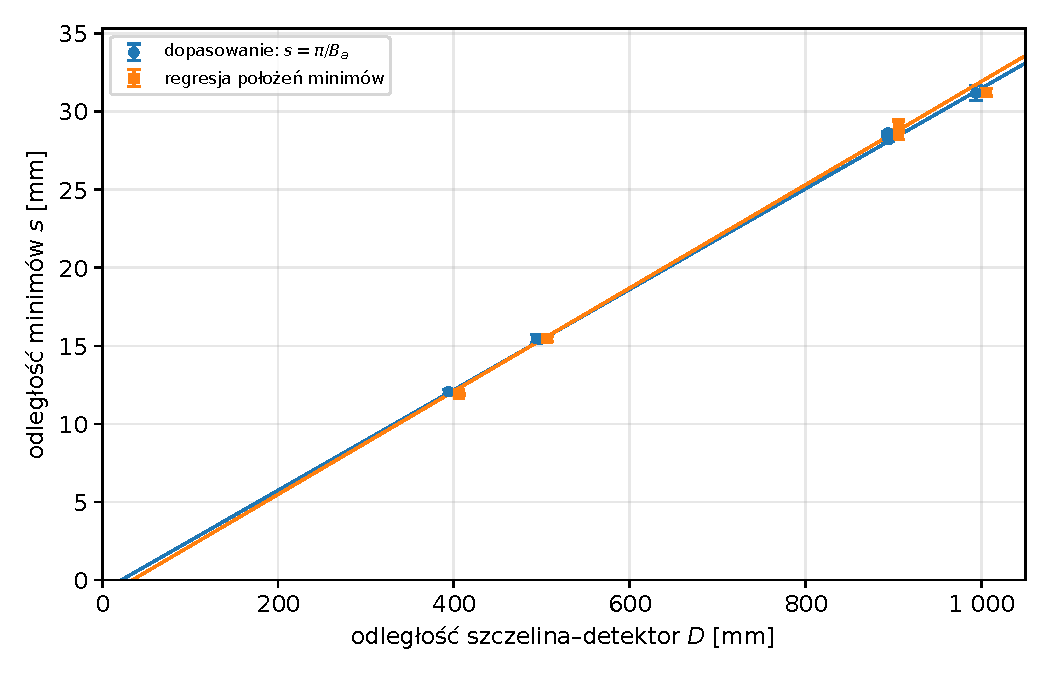
\includegraphics[width=0.72\textwidth]{distance_scaling.pdf}
    \caption{Odstęp minimów dyfrakcyjnych $s$ w funkcji odległości szczelina--detektor $D$
             ($a_\text{nom} = 0{,}02$~mm, laser czerwony) z prostymi~\eqref{eq:s_vs_D}
             dopasowanymi metodą najmniejszych kwadratów. Słupki błędów --- $u(s)$
             z dopasowania krzywej i z regresji położeń minimów.}
    \label{fig:distance_scaling}
\end{figure}

\subsection{Zmiana apertury czujnika}

Dopasowania dla obu apertur i apertury zwykłej przedstawiono na Rysunku~\ref{fig:aperture},
a parametry --- w Tabeli~\ref{tab:aperture}.

\begin{figure}[H]
    \centering
    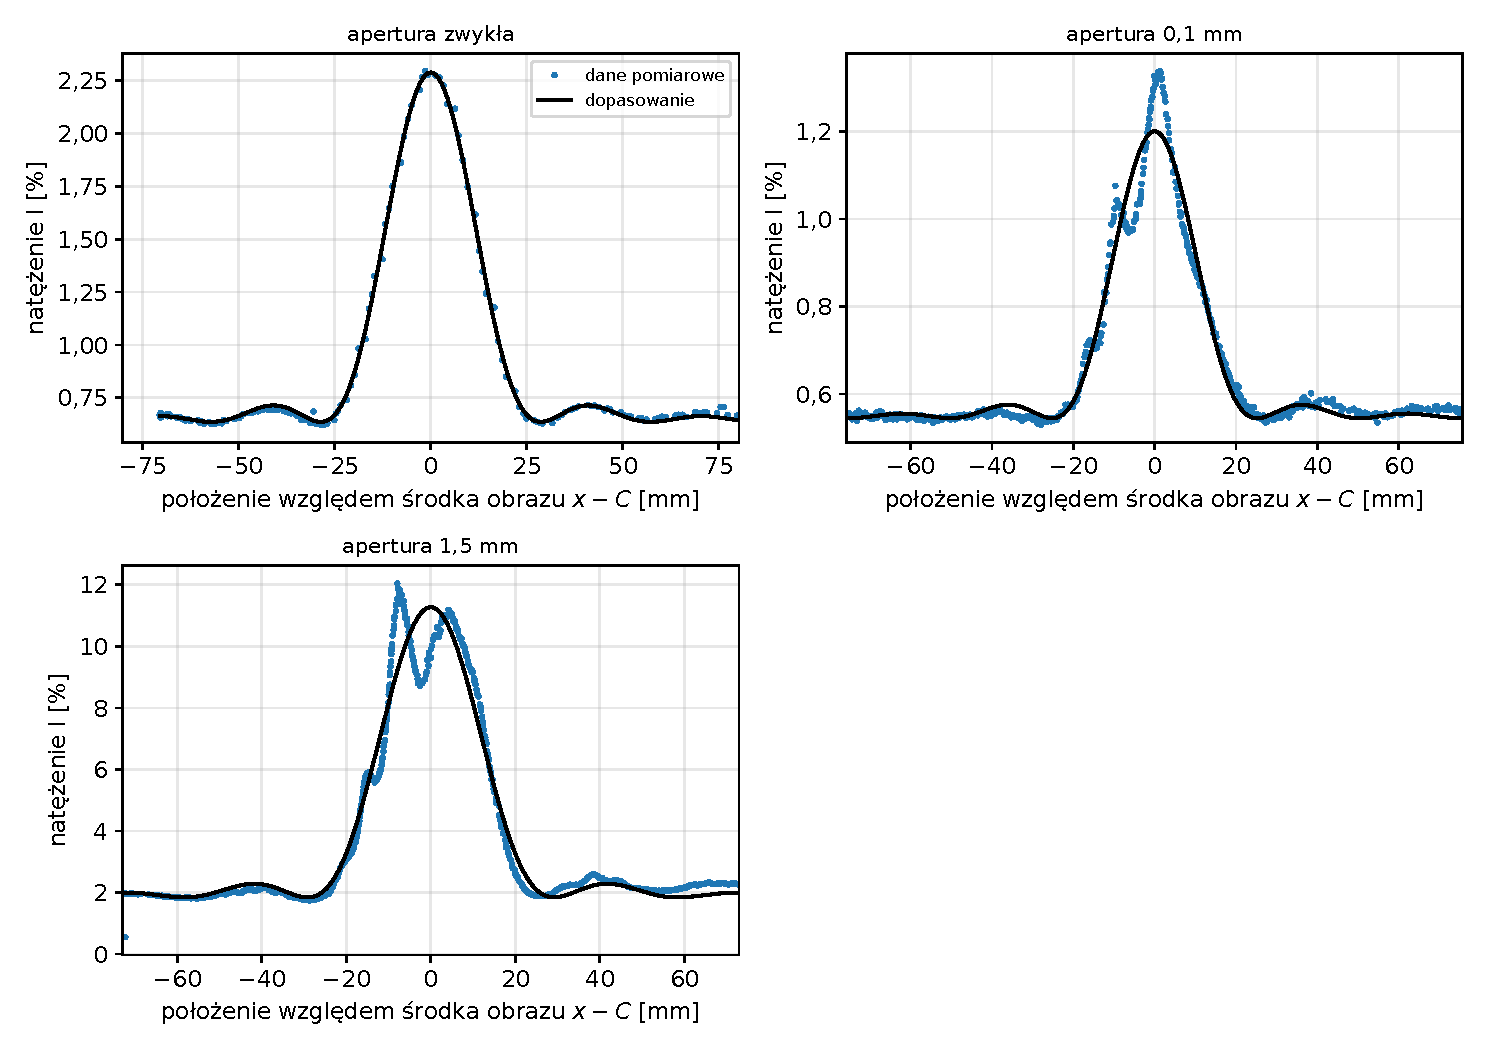
\includegraphics[width=0.9\textwidth]{aperture.pdf}
    \caption{Rozkład natężenia za szczeliną $a_\text{nom} = 0{,}02$~mm (laser czerwony,
             $D = 900$~mm) dla apertury zwykłej i apertur $0{,}1$ oraz $1{,}5$~mm z dopasowanym
             modelem~\eqref{eq:model_single} (linia ciągła).}
    \label{fig:aperture}
\end{figure}

\begin{table}[H]
    \centering
    \caption{Parametry dopasowania modelu~\eqref{eq:model_single} dla różnych apertur
             czujnika ($a_\text{nom} = 0{,}02$~mm): $B_a$, natężenie maksimum ponad tłem $A$,
             tło $b$ i RMS residuów względem $A$; dla apertury zwykłej trzy przejazdy.}
    \label{tab:aperture}
    \begin{tabular}{l S[table-format=1.5]@{\,$\pm$\,}S[table-format=1.5]
                    S[table-format=1.2] S[table-format=1.3] S[table-format=1.3]}
        \toprule
        apertura & \multicolumn{2}{c}{$B_a$ [mm$^{-1}$]} & {$A$ [\%]} & {$b$ [\%]} & {RMS$/A$} \\
        \midrule
        zwykła & 0.10970 & 0.00042 & 1.65 & 0.636 & 0.012 \\
        zwykła & 0.11138 & 0.00047 & 1.59 & 0.637 & 0.013 \\
        zwykła & 0.11084 & 0.00056 & 1.59 & 0.635 & 0.015 \\
        0,1    & 0.1247 & 0.0010 & 0.66 & 0.544 & 0.060 \\
        1,5    & 0.10753 & 0.00086 & 9.43 & 1.842 & 0.070 \\
        \bottomrule
    \end{tabular}
\end{table}

\paragraph{Szerokość apertur.} Obraz szczeliny $a = 0{,}02$~mm ($s \approx 28$~mm) jest dużo szerszy
od apertury, więc moc zebrana przez czujnik jest proporcjonalna do szerokości apertury $w$.
Natężenie ponad tłem przy szerszej aperturze wynosi $A = 9{,}43\,\%$, a przy $0{,}1$~mm
$A = 0{,}656\,\%$. Stosunek $14{,}4$ zgadza się ze stosunkiem szerokości $15$ dla apertury
$1{,}5$~mm, a nie z $7$ dla zapisanego w notatkach $0{,}7$ (oba przejazdy
wykonano jeden po drugim, przy tych samych ustawieniach). W ten sam sposób z porównania z aperturą
zwykłą (sesja 27 października, więc tylko orientacyjnie) wychodzi jej szerokość ok.\ $0{,}25$~mm,
czyli najpewniej $0{,}2$ lub $0{,}3$~mm; jej oznaczenia nie zanotowano.

\paragraph{Natężenie i tło.} Przy aperturze $1{,}5$~mm natężenie maksimum ponad tłem $A$ jest $5{,}8$ razy, a tło $2{,}9$ razy
większe niż przy zwykłej: szersza szczelina wejściowa zbiera więcej światła, także
rozproszonego. (Stosunek surowych $I_\text{max}$ z Tabeli~\ref{tab:scans_red}, $12{,}0/2{,}3 \approx 5$,
jest mniejszy, bo zawiera tło.) Przy aperturze $0{,}1$~mm natężenie spada do $A = 0{,}66\,\%$
ponad tłem $b = 0{,}54\,\%$: maksimum jest ok.\ $2{,}2$ razy wyższe od tła, a $A$ ok.\ $35$ razy
większe od szumu tła ($\sigma = 0{,}019\,\%$), więc sygnał jest dobrze mierzalny.

\paragraph{Szerokość obrazu.} Parametr $B_a$ zmienia się o $-2{,}8\,\%$ (apertura $1{,}5$~mm) i $+12{,}7\,\%$ (apertura $0{,}1$~mm)
względem średniej dla apertury zwykłej ($0{,}1106$~mm$^{-1}$, rozrzut przejazdów
$\sigma = 0{,}0009$~mm$^{-1}$, czyli $0{,}8\,\%$). Uśrednianie po szerokości apertury może obraz
tylko poszerzyć, czyli zmniejszyć $B_a$; wzrost $B_a$ przy węższej aperturze o $13\,\%$ jest więc
niefizyczny. Także spadek o $2{,}8\,\%$ przy $w = 1{,}5$~mm jest za duży jak na uśrednianie:
dla $w/s = 0{,}05$ splot zaniża $B$ o mniej niż $0{,}1\,\%$. Oba przejazdy mają zniekształcone maksimum centralne (RMS residuów $6$--$7\,\%$
wobec $1{,}2$--$1{,}5\,\%$), tak jak przejazdy z części zmiany odległości wykonane tego samego dnia,
i to zniekształcenie, a nie apertura, decyduje o dopasowanym $B_a$. Wpływu apertury na
szerokość obrazu nie da się z tych pomiarów wyznaczyć.

\subsection{Porównanie z wartościami producenta i porównanie laserów}
\label{sec:scale}

Stosunek $k = q/q_\text{nom}$ dla wszystkich wyznaczonych wielkości przedstawiono na
Rysunku~\ref{fig:scale}. Średnia ważona wyników z dopasowania (wagi $w_i = 1/u_{A,i}^2$; bez
$a$ z układów $N$ szczelin, obciążonego, zob.\ podsekcja Układy $N$ szczelin) wynosi
\begin{equation}
    k_\text{red} = 1{,}009 \pm 0{,}021, \qquad k_\text{green} = 1{,}036 \pm 0{,}022.
    \label{eq:k}
\end{equation}
Rozrzut wyników przekracza niepewności statystyczne: $\chi^2/\nu = 7{,}3$ (16 wielkości,
$k = 0{,}96$--$1{,}06$) i $4{,}1$ (7 wielkości, $k = 1{,}01$--$1{,}06$). Niepewność statystyczną
średniej powiększono więc o czynnik Birge'a $\sqrt{\chi^2/\nu}$ ($2{,}7$ i $2{,}0$), a następnie
dodano część systematyczną ($\lambda$, $D$, $K_x$). Rozrzut oznacza, że poszczególne szczeliny
odbiegają od wartości nominalnych także indywidualnie, o kilka procent (por.\ $s\,a_\text{nom}$
w podsekcji Pojedyncza szczelina). Po kalibracji skali wyniki są zgodne z wartościami producenta:
$|k - 1|/u(k) = 0{,}4$ (czerwony) i $1{,}6$ (zielony). Przy porównaniu laserów między sobą
$D$ i $K_x$ są wspólne i się znoszą; z samą częścią statystyczną i $u_\lambda$ różnica wynosi
$k_\text{green} - k_\text{red} = 0{,}027 \pm 0{,}015$ ($1{,}7\sigma$) --- zielone wyniki leżą
systematycznie nieco wyżej. To ta sama informacja co porównanie długości fal niżej. Bez kalibracji wyszłoby $k_\text{red} = 1{,}823$ i $k_\text{green} = 1{,}872$,
czyli tyle, ile wynosi $K_x = 1{,}807 \pm 0{,}016$ wyznaczone niezależnie z zakresu przesuwu
skanera --- dwie niezależne kalibracje skali dają ten sam czynnik.

\begin{figure}[H]
    \centering
    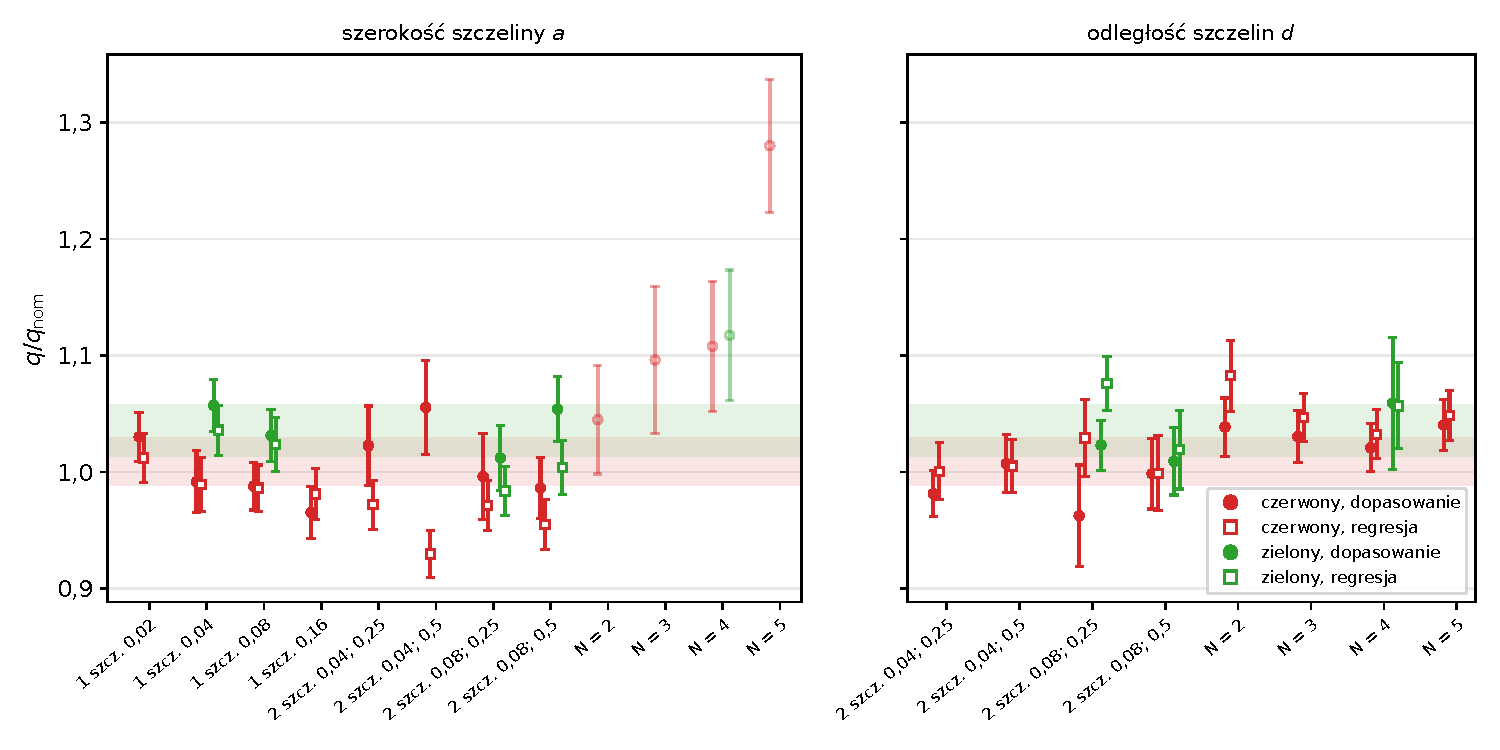
\includegraphics[width=0.95\textwidth]{scale_factor.pdf}
    \caption{Stosunek wyznaczonej wielkości do wartości producenta $q/q_\text{nom}$ dla
             wszystkich układów, obu laserów i obu metod, po kalibracji skali (pełne punkty ---
             dopasowanie, puste --- regresja; bladym kolorem $a$ z układów $N$ szczelin, pominięte
             w średniej); pasma --- średnia ważona~\eqref{eq:k} z niepewnością dla każdego lasera.}
    \label{fig:scale}
\end{figure}

Te same szczeliny zmierzono obydwoma laserami przy tym samym $D$ (uchwytów między sesjami
nie przesuwano). Parametr dopasowania $B = \pi q/(\lambda D)$ zależy od $\lambda$, a skala $x$
(także $K_x$) i $D$ są wspólne, więc w ilorazie się skracają:
\begin{equation}
    \lambda_\text{red} = \lambda_\text{green}\,\frac{B^\text{green}}{B^\text{red}}.
    \label{eq:lambda_red}
\end{equation}
Parametry $B_a$ i $B_d$ jednego układu pochodzą z tych samych przejazdów, więc nie są
niezależne; dla każdego układu uśredniono je do jednej wartości $\lambda_\text{red}$
(Tabela~\ref{tab:lambda}). Średnia ważona z pięciu układów wynosi
$\lambda_\text{red} = (680 \pm 9)$~nm. Na niepewność składają się część statystyczna
$5{,}4$~nm (większa z: niepewności średniej ważonej i rozrzutu układów; $\chi^2/\nu = 0{,}3$)
oraz $u(\lambda_\text{green})$, która daje $6{,}6$~nm i dominuje. Od wartości z tabliczki lasera
wynik różni się o
\begin{equation}
    \frac{|680{,}4 - 650|}{\sqrt{8{,}6^2 + 5^2}} = \frac{30{,}4}{9{,}9} \approx 3{,}1,
\end{equation}
czyli na samej granicy $3\sigma$ ($u(\lambda_\text{red}) = 8{,}6$~nm przed zaokrągleniem).
Porównanie mierzy jednak tylko stosunek długości fal:
$\lambda_\text{red}/\lambda_\text{green} = 1{,}321 \pm 0{,}011$ wobec $650/515 = 1{,}262 \pm 0{,}016$
z tabliczek (różnica $4{,}7\,\%$, $3{,}1\sigma$). Nie rozstrzyga ono, który laser odbiega od tabliczki:
równie dobrze $\lambda_\text{red} = 680$~nm przy $\lambda_\text{green} = 515$~nm, jak
$\lambda_\text{green} = 492$~nm przy $\lambda_\text{red} = 650$~nm. Czynniki $k$ (wzór~\eqref{eq:k})
nieznacznie wskazują na laser zielony: $k_\text{red}$ jest zgodne z 1, a wszystkie wyniki zielone
leżą wyżej ($k = 1{,}01$--$1{,}06$).

\begin{table}[H]
    \centering
    \caption{Długość fali lasera czerwonego ze wzoru~\eqref{eq:lambda_red} dla układów
             zmierzonych obydwoma laserami (średnie $B$ z trzech przejazdów); niepewność
             statystyczna z rozrzutu przejazdów, bez $u(\lambda_\text{green})$.}
    \label{tab:lambda}
    \begin{tabular}{l l S[table-format=3.1]@{\,$\pm$\,}S[table-format=2.1]}
        \toprule
        układ & parametry & \multicolumn{2}{c}{$\lambda_\text{red}$ [nm]} \\
        \midrule
        1 szczelina, $a = 0{,}04$~mm & $B_a$ & 693 & 13 \\
        1 szczelina, $a = 0{,}08$~mm & $B_a$ & 678.6 & 6.6 \\
        2 szczeliny, $a = 0{,}08$~mm, $d = 0{,}25$~mm & $B_a$, $B_d$ & 676 & 26 \\
        2 szczeliny, $a = 0{,}08$~mm, $d = 0{,}50$~mm & $B_a$, $B_d$ & 676 & 19 \\
        $N = 4$ szczelin & $B_a$, $B_d$ & 665 & 38 \\
        \bottomrule
    \end{tabular}
\end{table}

% -------------------------------------------
\section{Wnioski}
% -------------------------------------------

\subsection{Pojedyncza szczelina}

Szerokości szczelin wyznaczone dopasowaniem wynoszą (laser czerwony)
$a = (0{,}0206 \pm 0{,}0004)$, $(0{,}0397 \pm 0{,}0011)$, $(0{,}0790 \pm 0{,}0016)$
i $(0{,}1545 \pm 0{,}0036)$~mm dla $a_\text{nom} = 0{,}02$, $0{,}04$, $0{,}08$ i $0{,}16$~mm
oraz (laser zielony) $(0{,}0423 \pm 0{,}0009)$ i $(0{,}0825 \pm 0{,}0018)$~mm dla
$a_\text{nom} = 0{,}04$ i $0{,}08$~mm. Wszystkie są zgodne z wartościami producenta w granicach
$3\sigma$; dla lasera czerwonego odchylenia nie przekraczają $1{,}6\sigma$, a największe ($2{,}6\sigma$)
ma szczelina $0{,}04$~mm w świetle zielonym, zgodnie z ogólnie wyższymi wynikami tego lasera
(podsekcja~\ref{sec:scale_concl}). Regresja położeń minimów daje wyniki różniące
się od dopasowania o najwyżej $2{,}1\,\%$, mniej niż niepewność systematyczna, więc obie metody
są równoważne. Odstęp minimów skaluje się z $1/a$: przy ośmiokrotnej zmianie szerokości iloczyn
$s\,a_\text{nom}$ zmienia się o $7\,\%$ i leży w granicach $\pm4\,\%$ od $\lambda D$, co odpowiada
odchyleniom poszczególnych szczelin od wymiarów nominalnych o kilka procent.

\subsection{Dwie szczeliny}

Odległości między szczelinami z dopasowania wynoszą $d = (0{,}245 \pm 0{,}005)$
i $(0{,}504 \pm 0{,}012)$~mm ($a_\text{nom} = 0{,}04$~mm) oraz $(0{,}241 \pm 0{,}011)$
i $(0{,}499 \pm 0{,}015)$~mm ($a_\text{nom} = 0{,}08$~mm) dla $d_\text{nom} = 0{,}25$ i $0{,}50$~mm
(laser czerwony), a $(0{,}256 \pm 0{,}005)$ i $(0{,}505 \pm 0{,}014)$~mm dla lasera zielonego ---
wszystkie zgodne z wartościami producenta ($|d - d_\text{nom}|/u(d) \le 1{,}1$). Szerokości $a$
z dopasowania zgadzają się z wynikami dla pojedynczych szczelin.

Jedyna powtarzalna niezgodność metod dla $d$ dotyczy pary $a = 0{,}08$~mm, $d = 0{,}25$~mm:
regresja zawyża $d$ o $5\,\%$ (laser zielony, $z = 4{,}3$) i $7\,\%$ (czerwony, $z = 3{,}9$).
Przy $d/a = 3{,}1$ w maksimum obwiedni mieści się tylko 5 prążków ($m' = 0, \pm1, \pm2$), a skrajne
leżą na zboczu obwiedni $\left[\sin(B_a y)/(B_a y)\right]^2$: w obrębie prążka $m' = \pm2$
obwiednia spada ok.\ 8-krotnie, z $0{,}44$ do $0{,}06$ wartości maksymalnej. Mnożenie przez
malejącą obwiednię przesuwa wierzchołek prążka w stronę środka obrazu, zmniejsza zmierzony
odstęp $s$, a więc zawyża $d = \lambda D/s$. Dla par o $d/a = 6{,}25$ i $12{,}5$ zbocze obwiedni
jest łagodniejsze i metody różnią się o najwyżej $2\,\%$. Dlatego dla dwóch szczelin
wiarygodniejszy jest wynik dopasowania, które uwzględnia obwiednię jawnie.

\subsection{Układy $N$ szczelin}

Odległość $d = 0{,}128$--$0{,}130$~mm (laser czerwony, $d_\text{nom} = 0{,}125$~mm, odchylenia
$\le 1{,}9\,u(d)$) nie zależy od liczby szczelin, czyli położenia maksimów głównych są takie same
dla $N = 2$--$5$, zgodnie ze wzorem~\eqref{eq:young_max}. Między sąsiednimi maksimami głównymi
występuje $N - 2$ maksimów pobocznych, szerokość połówkowa maksimum głównego maleje od
$2{,}47$~mm ($N = 2$) do $0{,}87$~mm ($N = 5$) i zgadza się z przewidywaniem ze
wzoru~\eqref{eq:n_slits} w granicach niepewności ($z \le 2{,}2$), a natężenie maksimum głównego
rośnie jak $N^p$ z $p = 2{,}12 \pm 0{,}12$, zgodnie z $p = 2$. Obraz interferencyjny jest
modulowany obwiednią pojedynczej szczeliny o tej samej szerokości. Szerokość $a$ z dopasowania
układów $N$ szczelin jest obciążona: rośnie z $N$ (do $0{,}051$~mm dla $N = 5$), a dla $N = 5$
model nie odtwarza wysokości dalszych maksimów głównych (model ok.\ $3\,\%$ wobec zmierzonych
$12\,\%$ przy maksimum centralnym $71\,\%$). Zależy ona od wysokości kilku prążków, a więc od
oświetlenia poszczególnych szczelin, dlatego nie jest wynikiem.

\subsection{Zmiana odległości szczelina--detektor}

Odstęp minimów rośnie liniowo z odległością, $s = (\lambda/a)D + c$ z $R^2 = 0{,}9993$.
Szerokość szczeliny z nachylenia, $a = (0{,}0202 \pm 0{,}0004)$~mm, i z poszczególnych odległości
($0{,}020$--$0{,}022$~mm) nie zależy od $D$ w zakresie 400--1000~mm i zgadza się z wynikiem
dla $D = 900$~mm oraz z $a_\text{nom} = 0{,}02$~mm. Wyraz wolny $c = (-0{,}71 \pm 0{,}35)$~mm
odpowiada przesunięciu $\Delta D = (-22 \pm 11)$~mm, czyli $2\sigma$ od zera. Odczyt $D$ z ławy
może więc być przesunięty co najwyżej o $2$--$3$~cm, co jest zgodne z przyjętą niepewnością
$u_D = 14$~mm ($|\Delta D|/u_D = 1{,}6$).

W pomiarach z 3 listopada maksimum centralne jest rozdwojone (RMS residuów $4$--$6\,\%$ wobec
$1{,}3\,\%$ 27 października). Odstęp garbów rośnie z $D$ ($3{,}4$; $7{,}8$; $11{,}6$~mm dla
$D = 400$, $500$, $1000$~mm), ale nie proporcjonalnie ($0{,}28$; $0{,}50$; $0{,}37$ odstępu
minimów $s$), więc na podstawie tych trzech przejazdów nie da się ustalić, gdzie struktura
powstaje. Przyczyny nie wyznaczono. Szerokość obrazu, z której wyznacza się $a$, model
odtwarza mimo to poprawnie.

\subsection{Zmiana apertury czujnika}

Natężenie rośnie proporcjonalnie do szerokości apertury: apertura $1{,}5$~mm zbiera $14{,}4$ raza
więcej światła niż apertura $0{,}1$~mm, przy stosunku szerokości $15$. Tak też ustalono szerokość
szerszej apertury, której oznaczenie zasłaniała naklejka (w notatkach zapisano $0{,}7$). Z tej zależności apertura
zwykła ma szerokość ok.\ $0{,}25$~mm (najpewniej $0{,}2$ lub $0{,}3$~mm). Apertura $1{,}5$~mm zwiększa natężenie maksimum ponad tłem $5{,}8$ razy,
a tło $2{,}9$ razy, więc stosunek sygnału do tła rośnie dwukrotnie. Węższa apertura ($0{,}1$~mm) obniża natężenie
maksimum ponad tłem do $0{,}66\,\%$ (ok.\ $2{,}4$ razy mniej niż przy zwykłej), przy czym sygnał
jest nadal ok.\ $35$ razy większy od szumu tła. Wpływu apertury na szerokość obrazu nie
wyznaczono: dla węższej apertury $B_a$ wzrosło o $13\,\%$, co jest niemożliwe dla samego
uśredniania po aperturze (ono obraz tylko poszerza), więc zmiany $B_a$ w obu przejazdach
wynikają ze zniekształconego maksimum centralnego, widocznego we wszystkich pomiarach
z 3 listopada. Pomiar wykonano też omyłkowo na szczelinie $a = 0{,}02$~mm, której szeroki
obraz ($s \approx 28$~mm) jest mało czuły na uśrednianie po aperturze: nawet dla $w = 1{,}5$~mm
zmiana $B_a$ byłaby mniejsza niż $0{,}1\,\%$.

\subsection{Kalibracja skanera i porównanie laserów}
\label{sec:scale_concl}

Skaner w połączeniu z biblioteką \texttt{pasco} mierzył położenie niedokładnie: przelicznik
$\SI{0.01}{\meter}$ na 2000 impulsów enkodera zaniża przesunięcia
$K_x = 1{,}807 \pm 0{,}016$ raza, co wynika z porównania pełnego przesuwu głowicy (155~mm według
specyfikacji producenta) z zapisanym ($85{,}8$~mm; wszystkie przejazdy wykonano od ogranicznika
do ogranicznika). Czynnik jest wspólny dla wszystkich przejazdów: różna zapisana długość
przejazdów ($77{,}9$--$85{,}8$~mm) nie przekłada się na szerokość obrazu, więc wynika z miejsca
rozpoczęcia zapisu, a nie ze zmiennej skali. Bez kalibracji wszystkie szerokości
i odległości szczelin wychodziły $1{,}8$--$1{,}9$ raza za duże. Po skalibrowaniu skali
czynnikiem $K_x$ średni stosunek do wartości producenta wynosi $k_\text{red} = 1{,}009 \pm 0{,}021$
i $k_\text{green} = 1{,}036 \pm 0{,}022$, czyli wyniki są zgodne z wymiarami szczelin
($0{,}4\sigma$ i $1{,}6\sigma$). Kalibracja z zakresu przesuwu i kalibracja na szczelinach
producenta dają więc ten sam czynnik niezależnie od siebie. Nie jest on okrągłą liczbą --- przy
czynniku 2 pełny przesuw wynosiłby $172$~mm, więcej niż 155~mm ze specyfikacji. Przyczyną jest
błędna stała przelicznika w bibliotece: rzeczywisty krok enkodera to ok.\ $\SI{9}{\micro\meter}$,
zgodnie z rozdzielczością $0{,}01$~mm ze specyfikacji, a nie $\SI{5}{\micro\meter}$. Skala jest
wspólna dla wszystkich przejazdów, więc nie jest to losowa utrata impulsów.

Analiza kierunków przejazdu wykazała ponadto opóźnienie odczytu położenia względem natężenia
$\tau = (250 \pm 50)$~ms. Przesuwa ono cały obraz o $v\tau$; $a$ i $d$ wyznaczone z przejazdów
w obu kierunkach różnią się o $(-0{,}7 \pm 0{,}9)\,\%$ i $(+0{,}1 \pm 0{,}8)\,\%$, więc opóźnienie
nie wpływa na wyniki.

Porównanie obu laserów, w którym skala $x$ i $D$ się skracają, daje stosunek długości fal
$\lambda_\text{red}/\lambda_\text{green} = 1{,}321 \pm 0{,}011$, o $4{,}7\,\%$ większy niż z tabliczek
($1{,}262$), czyli $\lambda_\text{red} = (680 \pm 9)$~nm przy $\lambda_\text{green} = 515$~nm
($3{,}1\sigma$ od tabliczki). Porównanie nie wskazuje, który laser odbiega: równie dobrze może to być
$\lambda_\text{green} \approx 492$~nm przy $\lambda_\text{red} = 650$~nm, a wyższe o $1{,}7\sigma$ wyniki
z lasera zielonego ($k_\text{green} = 1{,}036$ wobec $k_\text{red} = 1{,}009$) nieznacznie wskazują
właśnie na laser zielony. Wynik leży na granicy $3\sigma$ i zależy od przyjętej tolerancji długości
fali, której producent nie podaje: dla tolerancji $\pm10$~nm obu laserów różnica spadłaby do
ok.\ $1{,}7\sigma$. Jedyne porównanie z tej samej sesji (układ $N = 4$) daje
$(665 \pm 38)$~nm, zgodne z tabliczką. Rozbieżności nie można więc rozstrzygnąć bez znajomości
rzeczywistych długości fal laserów.

Po kalibracji skali wszystkie zjawiska przewidziane przez teorię --- skalowanie obrazu
z $\lambda D/a$ i $\lambda D/d$, położenia maksimów głównych niezależne od $N$, $N - 2$ maksimów
pobocznych, zwężanie maksimów głównych i wzrost ich natężenia jak $N^2$ --- potwierdzono
ilościowo, a wyznaczone wymiary szczelin zgadzają się z wartościami producenta.

\begin{thebibliography}{9}
\bibitem{skrypt}
    \textit{Skrypt do I Pracowni Fizycznej}, ćwiczenie O18:
    Badanie zjawiska dyfrakcji i interferencji światła laserowego
\bibitem{dodatek}
    M.~Czaja, \textit{Ćwiczenie O18 --- Dodatek B. Badanie zjawiska dyfrakcji i interferencji
    światła laserowego}, I Pracownia Fizyczna, WFAiIS UJ
\bibitem{laser3b}
    3B Scientific, \textit{Diode Laser, 650 nm, red (U22000)}, specyfikacja,
    \url{https://3bscientific.com/gb/diode-laser-650-nm-red-1003201-u22000,p_870_14980.html}
    [dostęp: 3 listopada 2026]
\bibitem{pasco}
    PASCO scientific, \textit{Wireless Diffraction Scanner OS-8441}, specyfikacja produktu,
    \url{https://www.pasco.com/products/sensors/wireless/os-8441}
    [dostęp: 3 listopada 2026]
\end{thebibliography}

\end{document}
% =============================================
